\documentclass[a4paper,10pt]{book}

\usepackage[brazil]{babel}    % dá suporte para os termos na língua portuguesa do Brasil
\usepackage[T1]{fontenc}      % Lê a codificação de fonte T1 (font encoding default é 0T1).
\usepackage{lmodern}        % Fonte "Latin Modern", experimente no lugar de ae
\usepackage{times}
\usepackage{t1enc}         % Fonte "Times New", experimente no lugar de ae
%\usepackage[latin1]{inputenc}
\usepackage[utf8]{inputenc} % acentuação em UTF8 (comente as linhas de inputenc, fontenc e ae)
                              % Caso tenha problemas ao usar UTF-8, experimente \usepackage{ucs}
\usepackage{indentfirst}       % indenta os primeiros parágrafos
\usepackage{amssymb,amsmath}   % simbolos matemáticos providos pela AMS
\usepackage[dvipdfm]{graphicx} % para inclusão de figuras (png, jpg, gif, bmp)
\usepackage{graphics}          % figuras gráficas
\usepackage{color}             % para letras e caixas coloridas
\usepackage{makeidx}           % índice remissivo
\usepackage{a4wide}            % correta formatação da página em A4
\usepackage{setspace}          % para a distância entre linhas
\usepackage{html}
\usepackage{ulem}
\usepackage{longtable} %para tabelas longas
\usepackage{array}
\usepackage[table]{xcolor}
\usepackage{wrapfig}
\usepackage[pdftex]{hyperref}
\usepackage{longtable}

%\usepackage{minitoc}

\newcommand\atencao[1]{\textbf{}}

\makeindex

\title{Conte com Moodle no Próximo Semestre \\ \mbox{} \\ 
\includegraphics[width=2.0cm]{imagem/cap0/hat.jpg}}
\author{UFPB Virtual}
\date{April - 2013}

\begin{document}

\maketitle

\pagenumbering{roman}

\cleardoublepage
\begin{center}
\quad

\vspace*{0.9\textheight}

 \parbox[t]{0.7\textwidth}{Texto produzido para uso dos tutores e professores da UFPB Virtual.}
\parbox[t]{12cm}{Registrado sob licença Creative Commons (\url{www.creativecommons.org})}
\end{center}

\index{Ubuntu}
\index{Kile}
\index{Creative Commons}
\index{Moodle 1.9.3$^+$}

\tableofcontents
%\listoffigures

\mainmatter
\chapter{Introdução}

%\minitoc

Desde o início dos anos 90 professores ouvem comentários sobre a revolução que vem sendo provocada pela Internet no ensino e na aprendizagem, mas essa revolução ainda não se materializou. Em lugar disso, um novo conjunto de ferramentas, chamado LMS (Learning Management System em inglês, Sistema de Gestão de Aprendizagem em português), ou AVA como é mais conhecido (Ambiente Virtual de Aprendizagem), pode ser usado para melhorar seus cursos, tirando proveito das vantagens da Internet sem dispensar a necessidade do professor. Nos últimos dez anos, os AVAs experimentaram um crescimento e amadurecimento rápidos e são, hoje, considerados essenciais em muitas universidades e faculdades.

\index{Gestão da aprendizagem}

\section{Ambientes Virtuais de Aprendizagem}

AVAs são aplicações Intra/Internet que “rodam” em um servidor web\footnote{Servidor web é um computador que está ligado 7 dias na semana, 24 horas por dia, à Internet, onde estão gravados os arquivos do Ava e onde está um banco de dados que guarda as informações das disciplinas e usuários, podendo ser acessadas mediante autenticação, pelos interessados em qualquer lugar onde haja conexão com a rede mundial de computadores.}  e são acessadas por um navegador (Internet Explorer, Monzila Firefox, Google Chrome, Ópera, Safari, etc.). O servidor está, no caso geral, localizado em um departamento ou centro de processamento de uma Universidade, mas pode estar localizado em qualquer lugar do mundo. O professor e os alunos podem acessar o sistema de qualquer lugar onde haja um computador, conexão com a Internet e um navegador Web. Em termos simples, um AVA fornece ao professor ferramentas para que ele crie um curso baseado em uma ambiente Web (site), com controle de acesso de forma tal que somente os alunos do curso possam acessar o mesmo. Além deste controle, os AVAs oferecem uma variedade de ferramentas que podem aumentar a eficácia de um curso. Pode-se, facilmente, compartilhar materiais de estudo, manter discussões síncronas e assíncronas\footnote{Síncrona: que acontece em tempo real, ao mesmo tempo para todos os participantes. Assíncrona: que não está vinculada ao tempo, ou seja, a discussão pode ocorrer em períodos de tempo distintos, quando uma participação que ocorre agora é respondida depois e assim por diante.}, aplicar testes de avaliação e pesquisas de opinião, coletar e revisar tarefas, além de registrar notas. 

\index{síncrono}
\index{assíncrono}

\section{Recursos AVA}
\index{Recursos}
Os ambientes AVAs provêem os mais variados recursos educacionais, no intuito de prover maior didática e eficiência na comunicação entre alunos e professores.  Podemos analisar alguns destes recursos a seguir.

\subsection{Enviando e compartilhando materiais de estudo}
\index{Materiais de estudo}
A maioria dos AVAs fornece ferramentas para publicar com facilidade, textos e outros materiais de estudo. Ao invés de usar um editor HTML\footnote{Hypertext Markup Language: Linguagem de Marcação para Hipertextos, usada para dar formatação às páginas web e criar vínculos (links) entre elas.} , e então, enviar o texto para um servidor Web, usa-se um formulário para publicar conteúdos (enviar arquivos). Muitos professores costumam publicar em um site da Internet todo o material que produzem e que pode ser útil para os seus alunos. Porém estes ambientes não possuem tantos recursos didáticos como o ambiente AVA.


\subsection{Fóruns e Salas de bate-papo}

\index{Fóruns e chat}

Esses recursos fornecem meios de comunicação entre o professor e os alunos fora da sala de aula. Os fóruns proporcionam mais tempo para reflexão antes que a participação aconteça e permitem manter uma discussão por um período longo de tempo. As salas de bate-papo, por outro lado, fornecem uma forma de comunicação rápida e instantânea com professores, tutores e alunos. Podem ser usados para uma discussão aberta, com tema livre, ou até mesmo para uma aula virtual. Sabe-se de um professor que, impedido de falar por motivos médicos, conduz seu curso usando salas de bate-papo para se comunicar com os alunos. Outro uso comum é aquele feito por grupos de alunos que devem produzir um trabalho e usam o bate-papo online para se organizar e discutir detalhes do trabalho.

\subsection{Testes e pesquisas de opinião}

\index{Testes e pesquisas}

Testes online e pesquisas de opinião podem ser corrigidos e processados instantaneamente. São grandes ferramentas para permitir que os alunos tenham uma informação rápida e eficaz auto-avaliação sobre seu desempenho no curso. É comum hoje em dia que editoras e autores de livros texto coloquem questionários sobre os capítulos de seus livros em sítios na Internet. Podermos citar um exemplo de um professor que conduzindo um curso sobre propaganda na Universidade de São Francisco (EUA), produz um banco de questões e adota mini-testes para verificar o progresso dos alunos em seus estudos. A prova final é um teste com questões retiradas de todo o banco, de maneira aleatória.

\subsection{Coletando e revisando tarefas}

\index{Revisão de tarefas}

Coletar, corrigir e revisar tarefas (divulgando os resultados da correção com comentários) é um trabalho cansativo e maçante. Tarefas online é uma forma fácil de coletar e corrigir trabalhos dos alunos e atribuir e divulgar notas. Além disso, pesquisas indicam que o uso de ambientes online com participação anônima, para que os alunos atribuam notas a trabalhos feitos por seus colegas, aumenta a motivação e o desempenho.

\subsection{Registrando notas}

\index{Registro de notas}

Um quadro de notas online permite que os alunos tenham informações sempre atualizadas sobre seu desempenho em um curso. Notas online também facilitam cumprir a determinação de algumas instituições de ensino de que não tornem públicas as avaliações dos alunos. Os quadros de notas dos AVAs permitem, em geral, que os alunos consultem apenas as próprias notas. É possível, ainda, copiar o quadro de notas para o computador do professor para processamentos mais elaborados. Embora seja possível encontrar (ou desenvolver) programas que façam este trabalho, um AVA tem essas ferramentas integradas em seu ambiente. 

\section{Por que usar um AVA?}

Aulas têm sido ministradas por milhares de anos sem o uso de computadores ou da Internet. O ambiente em que o professor utiliza um quadro negro, giz e conversa ainda são ferramentas dominantes no processo educacional. Embora o formato tradicional, ou seja, de forma presencial, possa ainda ser eficaz, o uso das ferramentas acima listadas abrem novas possibilidades de aprendizagem que não eram imagináveis há anos atrás.

No momento, uma grande quantidade de pesquisa ainda é feita sobre como combinar aprendizagem presencial com os chamados cursos híbridos. Que são os cursos que combinam aulas presenciais e aula à distância. Imagine transferir a maior parte do material didático de seu curso para um ambiente virtual e aproveitar seu tempo em aula para discussões, questões e resolução de problemas. Muitos professores já descobriram que eles podem economizar tempo e melhorar a aprendizagem de seus alunos comportando-se dessa maneira. Isto permite que os alunos usem os encontros presencias para a solução de problemas e os professores possam transformar suas aulas em palestras de contextualização, abandonando a preocupação de ter que cumprir o programa de forma presencial.

As discussões online permitem que muitos alunos se expressem em formas que eles não conseguiriam em aulas regulares. Muitos deles relutam em falar em aula por motivos variados: timidez, insegurança, ou mesmo limitações de linguagem. A possibilidade de criar um ambiente de construção coletiva do conhecimento online é, muitas vezes, de grande importância para alguns alunos. Muitos professores relatam um aumento significativo na participação quando se introduz esse formato de aprendizagem. Há outro número de razões para se pensar na utilização de ambientes virtuais em seus cursos, como por exemplo:

\begin{itemize}
 \item Demanda dos alunos: os alunos (especialmente os de curso superior) têm, hoje, um grau de inclusão digital muito maior, e utilizam muitos sistemas de comunicação como (MSN, Facebook, GTalk, Skype, por exemplo) eles se sentem à vontade em um AVA;
 \item Horários dos alunos: aumenta cada vez mais o número de alunos que trabalha. Em alguns países, a média semanal de trabalho dos alunos de cursos superiores chega a 20 horas. Com ambientes online eles podem adequar seus horários de trabalho às atividades de um curso;
 \item Cursos melhores: se bem usado, um AVA pode tornar suas aulas mais eficazes e melhores. Movendo parte de seu curso para a Internet é possível aproveitar os encontros presenciais para envolver os alunos em questões básicas do curso e convidá-lo a refletir sobre temas correlatos. O professor pode, também, aproveitar o tempo discorrendo sobre temas que sempre desejou abordar e foi impedido pelo fato de ter que cumprir o programa.
\end{itemize}

Você provavelmente ouviu os argumentos até aqui apresentados durante a última década do século XX. Então, o que mudou? Hoje, os AVAs estão melhores estruturados, mais maduros, e fáceis de usar do que foram há alguns anos atrás. A tecnologia que envolve a disponibilidade deste ambiente tornou-se melhor e mais estável. Há pouco tempo, muitos sistemas eram projetados para uso pessoal, ou para uso de um grupo específico de pessoas, e eram comercializados na forma original, mostrando-se pouco flexíveis. Dois dos sistemas mais conhecidos (Blackboard e WebCT) começaram como projetos para pequenas faculdades e se tornaram líderes do mercado.

Entretanto, liderar o mercado não significa ser o melhor ou mais bem projetado. De fato, os líderes de mercado têm tido dificuldades para manter seu crescimento e argumenta-se inclusive que o esforço para manter essa liderança tem prejudicado a qualidade final do produto.



\section{Por que o Moodle é diferente?}

Muitos administradores de ambientes de aprendizagem têm declarado sua adesão ao Moodle principalmente em virtude de ser ele um sistema aberto baseado em uma forte filosofia educacional com uma comunidade de usuários que cresce dia a dia e contribui para o desenvolvimento e apoio a novos usuários. A seguir podem-se analisar detalhadamente algumas vantagens do AVA Moodle.

\section{Gratuito e de fonte aberta (código aberto)}

A expressão fonte aberta (do inglês open source) tornou-se um termo restrito a certo círculo de pessoas. Para aqueles que não estão acostumados com a linguagem técnica é difícil entender como essa idéia estranha e poderosa mudou para sempre o mundo do desenvolvimento de programas para computador. A idéia em si é bastante simples: fonte aberta significa que os usuários têm acesso ao código fonte do programa. Pode-se examinar (alterar, ampliar, modificar) o programa ou mesmo usar partes dele para aplicações de interesse pessoal.

Programas para computador de fonte aberta adotam valores acadêmicos de liberdade, avaliação pelos pares e compartilhamento do conhecimento. Qualquer pessoa pode baixar o Moodle gratuitamente, modificar ou acrescentar módulos, corrigir erros, melhorar seu desempenho ou simplesmente aprender observando como outras pessoas usam o ambiente e resolvem problemas. Alem disso, ao contrário dos sistemas proprietários, o Moodle pode ser instalado sem nenhum custo (em quantos servidores você desejar). Ninguém poderá retirá-lo de você, aumentar os custos de manutenção ou fazê-lo pagar por atualizações. Ninguém pode forçá-lo a fazer atualizações, comprar ferramentas que você não deseja ou determinar quantos usuários você pode ter.


\section{Pedagogia}

O criador do Moodle, Martin Dougiamas, tem formação em educação e informática. Isto o conduziu a adotar o Construcionismo Social como a estrutura pedagógica em que está baseado o ambiente. Isto é inovador uma vez que os ambientes de gestão de aprendizagem são, em geral, construídos em torno de ferramentas computacionais. Pode-se afirmar que os AVAs comerciais são voltados para ferramentas enquanto o Moodle é voltado para aprendizagem. O Construcionismo Social baseia-se na idéia de que pessoas aprendem melhor quando engajadas em um processo social de construção do conhecimento, pelo ato de construir alguma coisa para outros. Este é um conceito um tanto sintético que pode ser mais bem detalhado. O termo processo social sugere que a aprendizagem é alguma coisa que se faz em grupos. Deste ponto de vista, aprendizagem é um processo de negociação de significados em uma cultura de símbolos e artefatos compartilhados. O processo de negociação de significados e utilização de recursos compartilhados é o processo de construção do conhecimento. Nós não somos um quadro branco quando entramos no processo de aprendizagem. Nós precisamos testar nossos novos conhecimentos comparando-os com velhas crenças e incorporando-os em nossas estruturas de conhecimento já existentes. Parte do processo de teste e negociação envolve a criação de artefatos e símbolos para que outros interajam com eles.

E como isto tem relação com o ambiente Moodle? A primeira indicação está na interface. Enquanto AVAs centrados em ferramentas fornecem uma lista de ferramentas como sendo a interface, o ambiente Moodle coloca as ferramentas em uma interface que faz da aprendizagem a tarefa central. Pode-se estruturar um curso no ambiente Moodle nos formatos semanal, tópicos ou social. Além disso, enquanto outros AVAs se estruturam em um modelo de conteúdo que encoraja os professores a carregar uma infinidade de conteúdos estáticos, o ambiente Moodle enfoca o trabalho em ferramentas para discussão e compartilhamento de experiências. Assim, a ênfase está não em distribuir informação, mas em compartilhar idéias e engajar os alunos na construção do conhecimento.

A filosofia de projeto do Moodle torna-o um pacote amigável para professores e representa a primeira geração de ferramentas educacionais realmente úteis.

O Moodle tem uma comunidade de usuários grande e com participação na manutenção da distribuição, sugerindo sempre modificações, novas habilidades e reportando eventuais defeitos. Pode-se acessar a comunidade em  \url{http://moodle.org/}(em inglês) e no ambiente de discussão do Moodle Brasileiro em \url{http://moodle.org/?lang=pt_br em português}.

A comunidade Moodle tem sido indispensável para o sucesso do sistema. Com tantos usuários em todo o mundo sempre há alguém que pode responder a perguntas e dar conselhos. Ao mesmo tempo, os desenvolvedores e usuários do Moodle trabalham juntos para garantir qualidade, adicionar novos módulos e ferramentas e sugerir novas idéias de desenvolvimento do ambiente. Martin Dougiamas e sua equipe são responsáveis pela decisão de aceitar ou não as sugestões dos colaboradores. Em virtude do fato do ambiente ser de fonte aberta muitas pessoas desenvolvem novos módulos e os submetem à apreciação dos desenvolvedores e da comunidade. Isto funciona como um grande departamento de desenvolvimento e controle de qualidade.

Essas três vantagens - fonte aberta, Construcionismo Social e comunidade de desenvolvimento - fazem do Moodle um espaço de aprendizagem único no mundo.

                                                     \begin{flushright}Adaptação do texto do prof. Athail Rangel Pulino Filho
                                                      
                                                                                 Universidade de Brasília, DF\end{flushright} 
                                                                                 


\chapter{Acesso ao Moodle da UFPB Virtual}
Neste capítulo apresentaremos como professores e tutores poderão acessar o Moodle da UFPB Virtual, e como deverão prosseguir na navegação do mesmo.
\section{Informações importantes}
O acesso ao Ambiente de Educação à Distância pode ser feito de duas formas: ou diretamente no sítio \url{http://www.ead.ufpb.br}, ou 
clicando no botão \textbf{Acesso ao Moodle EAD} na página da UFPB Virtual \url{http://portal.virtual.ufpb.br}, como apresentado na Figura \ref{fig:apresentacao}.

\begin{figure}[htbp]
 \begin{center}
 \fbox{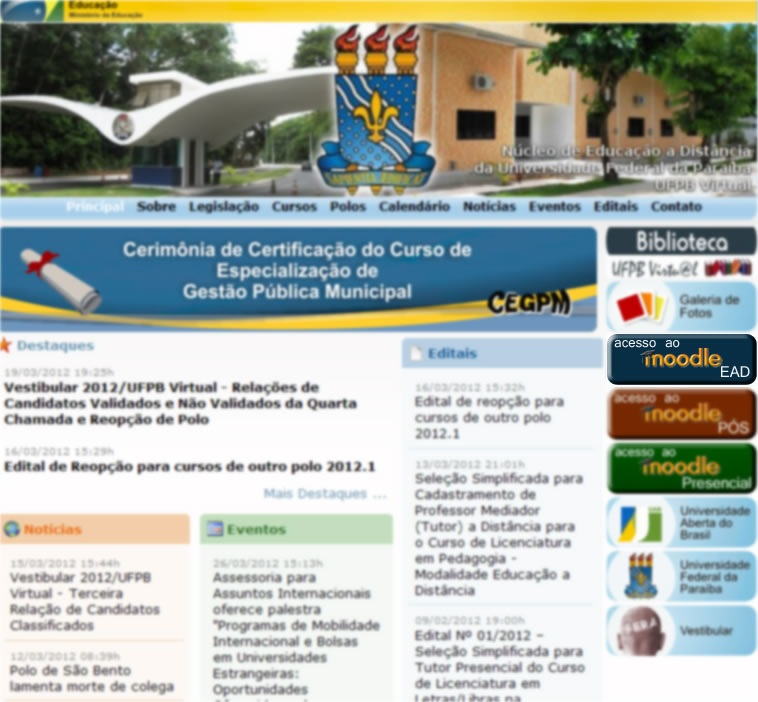
\includegraphics[width=0.5\textwidth]{imagem/cap2/fig1.jpg}}
  \caption{Site da UFPB Virtual}
  \label{fig:apresentacao}
 \end{center}
\end{figure}

Após o acesso pode-se também adicionar o site aos Favoritos do navegador, para que o endereço possa ser revisitado rapidamente. 
Estando na página de acesso do Moodle, basta clicar em  Favoritos, no menu do navegador.

Ao utilizar algum serviço de busca na Internet, como o Google, Yahoo, Ask, Bing, etc, deve-se ter o cuidado de verificar se o endereço acessado é o mesmo mencionado acima, pois os resultados da busca podem trazer também outras plataformas da UFPB Virtual, cujos cadastros não são compartilhados. Por exemplo, os sites do Moodle Presencial e do Moodle Pós-Graduação.
\section{Fazendo login}
\label{chap2:sec:login}
\index{Login}
A página de acesso o conteúdo da plataforma virtual está illustrada na Figura \ref{fig:login}. Em particular, para acessar o  

Para o acesso do conteúdo exposto na plataforma virtual é necessário a realização do login.
Para isso é necessário o preenchimento de dois campos obrigatórios pelo usuário, illustrados 
na Figura~\ref{fig:login}: o Nome de usuário e a Senha.

\begin{figure}[htbp]
 \begin{center}
 \fbox{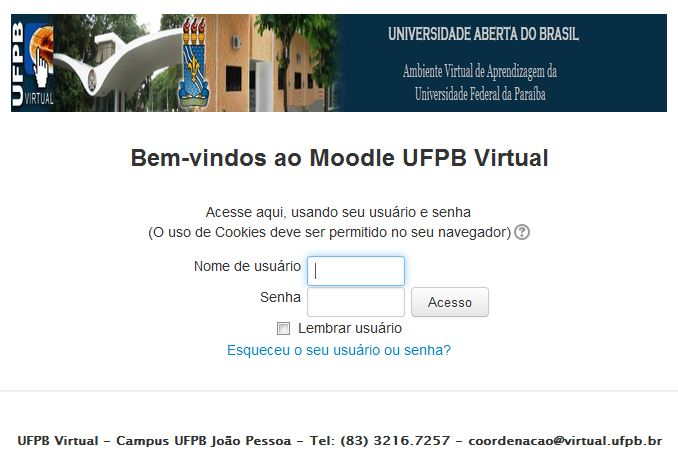
\includegraphics[width=0.8\textwidth]{imagem/cap2/fig2.jpg}}
  \caption{Página de acesso a Plataforma}
  \label{fig:login}
 \end{center}
\end{figure}

No Ambiente Virtual da UFPB, o cadastro dos usuários é realizado de tal forma que cada usuário tenha somente 
um cadastro. Para isso, os alunos utilizam como nome de usuário o \emph{número de matrícula}, os tutores o \emph{número de CPF} (Cadastro de Pessoa Física), enquanto que os professores e os coordenadores de pólo e curso o seu \emph{número de SIAP} (Sistema Integrado de Administração de Pessoal).

Para os usuários que acessam a plataforma pela primeira vez, o procedimento adotado é o preenchimento do campo Senha com a mesma informação utilizada para o campo Nome de Usuário. Por exemplo, um tutor que acessa a plataforma pela primeira vez deverá 
usar o seu CPF tanto como Login como a sua Senha.
\section{Trocando a senha}
\label{chap2:sec:trocando}
\index{Trocando senha}
Como visto na Seção~\ref{chap2:sec:login}, o usuário em seu primeiro acesso utilizará como senha o seu nome de usuário. Por motivos de segurança estes serão redirecionados para uma nova página, como pode ser visto na Figura \ref{fig:modifica senha}, em que necessitará o preenchimento de três campos. O campo \textbf{Senha atual} que corresponde ao nome de usuário utilizado, o campo \textbf{Nova senha} que deverá ser preenchido com a senha que o usuário adorará para acessar plataforma, não podendo ser igual ao nome de usuário, e o terceiro e último campo que requer a repetição da informação fornecida no campo \textbf{Nova senha}.

\begin{figure}[htbp]
 \begin{center}
 \fbox{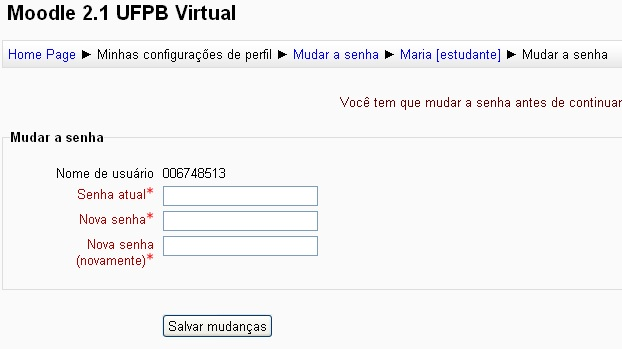
\includegraphics[width=0.6\textwidth]{imagem/cap2/fig3.jpg}}
  \caption{Página de modificação de senha}
  \label{fig:modifica senha}
 \end{center}
\end{figure}

Da mesma forma o usuário poderá atualizar sua senha, através do menu \textbf{Configurações} na seção \textbf{Minhas configurações de perfil}, como destacado na Figura \ref{fig:menu senha}.

\begin{figure}[htbp]
 \begin{center}
 \fbox{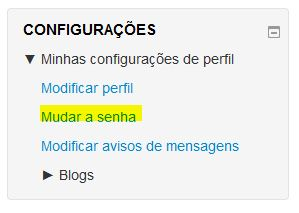
\includegraphics[width=0.3\textwidth]{imagem/cap2/fig4.jpg}}
  \caption{Menu para modificação de senha pelo usuário}
  \label{fig:menu senha}
 \end{center}
\end{figure}

\section{Recuperando a senha}
\index{Recuperando senha}
Caso o usuário tenha esquecido sua senha ou seu nome de usuário, a recuperação pode ser realizada através do link \textbf{Esqueceu o seu nome de usuário ou a sua senha? }disposto abaixo do campo \textbf{Senha} na página principal da plataforma, como visto na Figura \ref{fig:login}. Ao acessar este link, o usuário será direcionado para a página representada na Figura \ref{fig:recupera senha}.

\begin{figure}[htbp]
 \begin{center}
 \fbox{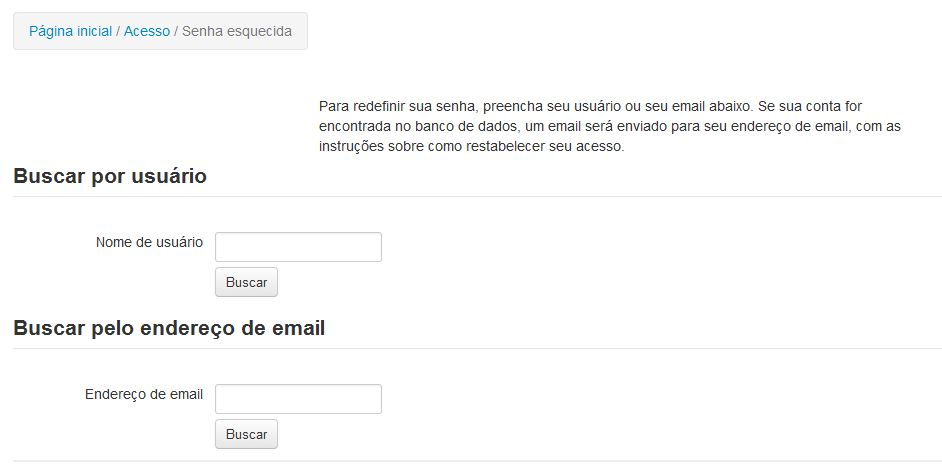
\includegraphics[width=0.6\textwidth]{imagem/cap2/fig5.jpg}}
  \caption{Página de recuperação de senha}
  \label{fig:recupera senha}
 \end{center}
\end{figure}
Nesta página há dois campos: \textbf{Nome de usuário} e \textbf{Endereço de e-mail}, que não necessita de preenchimento simultâneo, sendo apenas necessário um com a informação cadastrada no sistema Moodle. Caso o usuário informe o nome de usuário ou e-mail, é necessário que em seu cadastro o campo e-mail esteja preenchido corretamente, já que uma senha temporária será enviada a este e-mail. A senha temporária lhe dará acesso à plataforma e pedirá o usuário por uma nova senha da mesma forma descrita na Seção~\ref{chap2:sec:trocando}. 
Caso o usuário encontre dificuldades em realizar essa operação, o mesmo deve entrar em contato com o suporte através do e-mail \url{suporte@virtual.ufpb.br}, informando seus dados e informando o ocorrido.

\section{Guia de navegação no Moodle}
Ao entrar no ambiente o usuário visualizará a página inicial do Moodle, como illustrada na Figura \ref{fig:inicio}.

\begin{figure}[htbp]
 \begin{center}
 \fbox{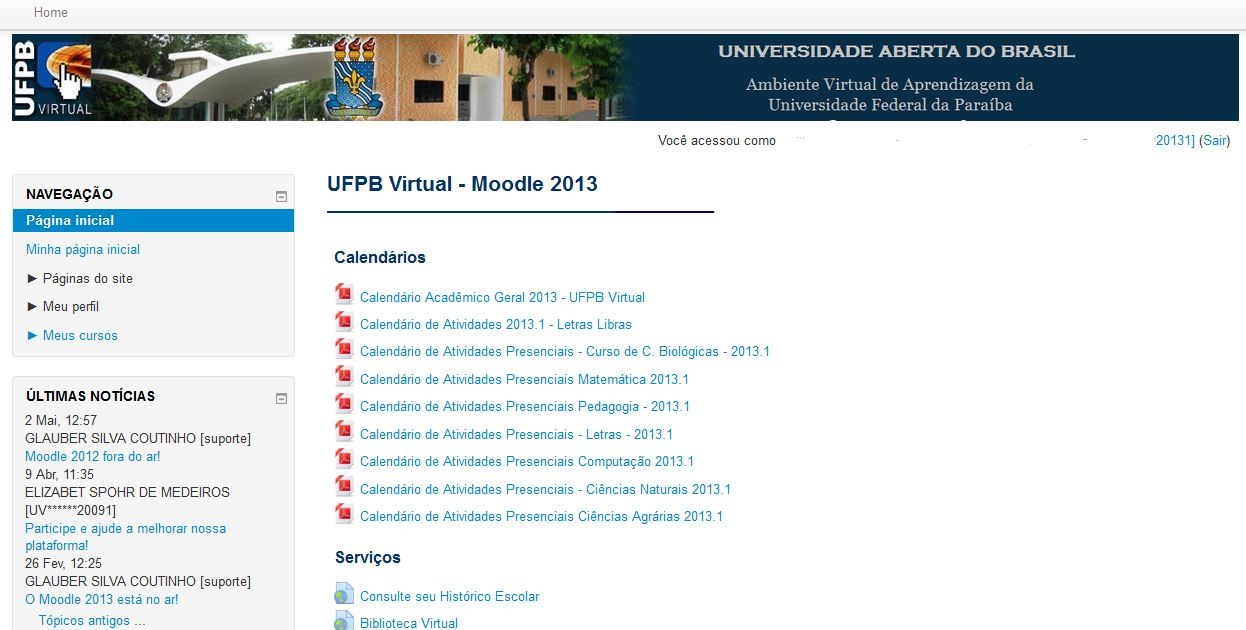
\includegraphics[width=0.6\textwidth]{imagem/cap2/fig6.jpg}}
  \caption{Página inicial}
  \label{fig:inicio}
 \end{center}
\end{figure}
A página inicial do Moodle possui duas colunas. Do lado esquerdo os blocos geralmente relacionados à configuração do Moodle e os blocos de conteúdo geral. Na coluna da direita, mais ampla, se encontram informações institucionais e acadêmicas e, abaixo dessas, a lista dos cursos aos quais o usuário está vinculado. Essa página varia um pouco conforme a \emph{função} do usuário no ambiente.

\begin{figure}[htbp]
 \begin{center}
 \fbox{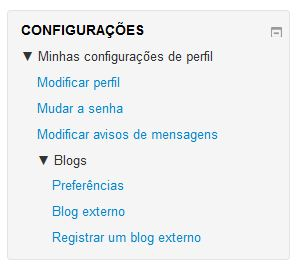
\includegraphics[width=0.3\textwidth]{imagem/cap2/fig7.jpg}}
  \caption{Configurações disponíveis}
  \label{fig:conf disp}
 \end{center}
\end{figure}


Como função pode-se entender o nível de permissões que o usuário possui. Um professor verá mais funcionalidades e recursos que um tutor, que por sua vez tem mais privilégios que um estudante. No entanto, o padrão descrito acima vale para qualquer tipo de usuário. As configurações disponíveis para um professor ou tutor são de alteração do perfil e gerenciamento das mensagens. A Figura~\ref{fig:conf disp} apresenta algumas das configurações disponíveis.


O perfil público do usuário também pode ser acessado clicando no seu nome, no alto de qualquer página do lado direito, dessa forma é possível acessar seu perfil o que permite edições do perfil, etc. Do lado esquerdo vê-se o \textbf{Calendário} e, eventualmente, o \textbf{bloco de últimas notícias}, como demonstrado na seguinte Figura.

\begin{center}
 \fbox{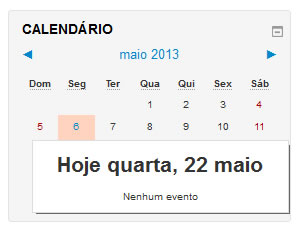
\includegraphics[width=0.2\textwidth]{imagem/cap2/fig8.jpg}}
\end{center}

No calendário passa-se o cursor sobre as datas e uma pequena janela será mostrada com os eventos marcados para esse dia, caso haja algum. Na página inicial o calendário mostrará todos os eventos globais, ou seja, aqueles eventos que envolvem todos os usuários na plataforma, como illustra a seguinte Figura:

\begin{center}
 \fbox{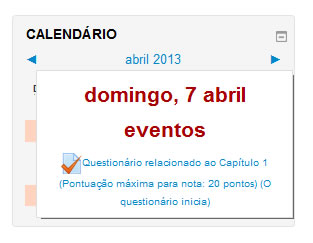
\includegraphics[width=0.2\textwidth]{imagem/cap2/fig9.jpg}}
\end{center}


\subsection{Configurando seu perfil}
\index{Configuração de perfíl}
Na tabela a seguir são demonstrados todos os campos disponíveis para modificação e o que eles representam.

\begin{longtable}{p{4cm}|p{9cm}}
\hline
   \rowcolor[rgb]{0.8,0.8,0.8}  \textbf{Campo} & \textbf{Descrição}\\
    \hline
    Nome  & Seu nome. Esse campo não pode ser editado. \\\hline
    Código de Usuário & Campo não editável. Contém um código que fornece informações sobre o usuário. Ex.: [PRAGR] significa:  Professor -  Curso de Ciências Agrárias  \\\hline
    Endereço de email & O endereço de e-mail. É um campo de preenchimento obrigatório. O e-mail é um importante meio de contato em um curso à distância, além de ser usado para resgatar sua senha, caso a tenha esquecido. (Veja Seção~\ref{chap2:sec:trocando}.) \\\hline
    Mostrar endereço de email & Permite escolher entre as seguintes opções: (1) somente os \textbf{Participantes} das suas disciplinas vejam seu e-mail, (2) que todos vejam, (3) que ninguém veja. O padrão é que somente os \textbf{Participantes} da disciplina possam ver seu endereço de e-mail. \\\hline
    Formato de email & Permite escolher entre receber mensagens em formato \textbf{HTML}, que possui formatação de fontes, cores de fundo, imagens, etc. e formato \textbf{TEXTO}, que somente possui os caracteres de texto, sem nenhuma formatação. \\\hline
    Email do tipo compilado & Configura o modo como se recebe as mensagens informando das postagens nos fóruns dos quais se é assinante. Sem compilação faz com que se recebam todas as participações, cada uma em uma mensagem separada. Completo envia um email diário com as participações completas. Assuntos envia uma mensagem diária com o resumo das participações. \\\hline
    Assinatura automática & Pode-se tornar assinante automaticamente em todos os fóruns dos quais se participa, ou não ser assinante automaticamente, mas fazer a opção manual, um a um. \\\hline
    Monitoramento do fórum & Permite optar entre visualizar na página principal da disciplina se existem mensagens não lidas nos fóruns. 
%     \textbf{Não, não marque}... \textbf{Não mostrará nada e Sim}, ponha em evidência para que seja possível ler as mensagens não lidas. 
    \\\hline
    Ao editar o texto & A opção \textbf{Usar o editor de HTML} permite o editor de texto nas atividades, configurações, etc. do Moodle formatar textos, incluir imagens, cores e outros recursos gráficos. A opção \textbf{Use formulários web} mostrará somente um campo de texto, onde será possível somente escrever em texto puro, sem nenhum outro recurso. \\\hline
 
%  Ajax e javascript & A opção \textbf{Não, use as características básicas da web} permitirá somente o uso de recursos básicos nas páginas do Moodle, em HTML. A opção \textbf{Sim: use as características avançadas da web} permitirá o uso de recursos que tornam mais rica a navegação, porém que exigirão mais do computador do usuário. Portanto sugerimos que computadores antigos usem a primeira opção. \\\hline
%  
%  Leitor de tela & Essa opção serve para quando o Moodle possui um aplicativo especial instalado que permita a leitura de tela, como elemento de acessibilidade para deficientes visuais. Caso um recurso assim esteja sendo utilizado, deixa-se marcado como SIM, caso não exista, deixa-se marcado como NÃO. Marcando SIM fará com que algumas atividades, como os chats, não abram usando frames ou javascript, de modo a proporcionar um ambiente favorável aos leitores de tela. \\\hline
%  
 Cidade/Município & Campo de preenchimento obrigatório. Deve ser informada a cidade onde reside o usuário. \\\hline
    Selecione um país & O país padrão é o Brasil. Caso seja outro deve ser selecionado. O preenchimento é obrigatório. \\\hline
    Zona de fuso horário & Esse campo definirá o horário em que o usuário está. O padrão é deixar o servidor gerenciar isso. Pode alterar as atividades com horário marcado. \\\hline
    Idioma preferido & Configura o idioma de predileção do usuário. O padrão é Português - Brasil (pt\_br). O Moodle reconhece essa escolha e abre a plataforma no idioma preferido, entre os que estiverem disponíveis. \\\hline
    Descrição  & Um campo de texto onde uma descrição do usuário pode ser editada. Essa descrição aparecerá no perfil público. \\\hline
    Imagem do Usuário & 1. Para excluir uma imagem, seleciona-se a caixa ao lado de Excluir, salvando após.
    \\
    & 2. Para enviar uma imagem clica-se em Escolha um arquivo, procura-se a imagem no próprio computador, dando ok. Ao sair da página de edição do perfil, Salvar. \\
    & 3. No campo Descrição da imagem escreve-se uma breve descrição que aparecerá ao passar o cursor sobre a imagem (nome da pessoa, etc). \\\hline
    Lista de Interesses & Permite ao usuário publicar uma lista de interesses pessoais, ou profissionais, que aparecerão em seu perfil público. Essa lista deve conter itens separados por vírgulas. \\\hline
    Página web & Permite publicar um endereço de site pessoal no perfil público do usuário. \\\hline
    Número de ICQ & Permite publicar um número de ICQ no perfil público do usuário. \\\hline
    ID Skype   & Permite publicar o id do Skype no perfil público do usuário. \\\hline
    AIM ID     & Permite publicar o id do AOL Instant Messenger no perfil público do usuário. \\\hline
    ID Yahoo   & Permite publicar o id do Yahoo no perfil público do usuário. \\\hline
    ID MSN     & Permite publicar o id do MSN no perfil público do usuário. \\\hline
    Número de identificação & Somente editável quando vazio. Deve conter o Siape do professor, CPF do tutor, ou a matrícula do aluno. \\\hline
    Curso (cod.) & Código do curso. Campo não editável para o usuário. \\\hline
    Função (cod.) & Nome da função (professor, tutor a distância, estudante). Não editável. \\\hline
    Fone, celular e endereço & Campos para publicação de informações pessoais do usuário, expostas no perfil público. \\\hline
    \label{tab:addlabel}
\end{longtable}%

% \subsection{Novidade apresentada pela nova versão do Moodle}
% 
% Recentemente foi acrescentada ao Moodle, nas versões acima de 2.0, foi a possibilidade de mover o bloco para a lateral esquerda da tela do monitor, deixando a área de trabalho do ambiente livre. Esse arranjo é ligado ao perfil do usuário, não trazendo mudança na maneira como os outros veem a página. Conforme pode ser visto nas Figuras \ref{fig:cap2_10} e \ref{fig:cap2_11}.
% 
% \begin{figure}[htbp]
%  \begin{center}
%  \fbox{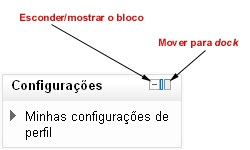
\includegraphics[width=0.3\textwidth]{imagem/cap2/fig10.jpg}}
%   \caption{Movendo blocos}
%   \label{fig:cap2_10}
%  \end{center}
% \end{figure}
% 
% 
% \begin{figure}[htbp]
%  \begin{center}
%  \fbox{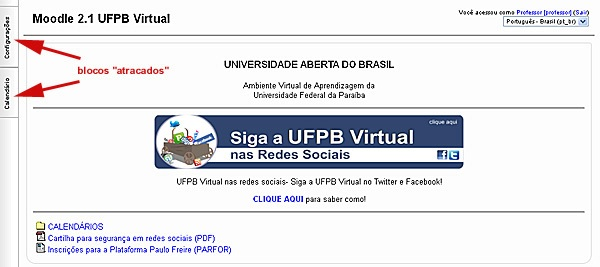
\includegraphics[width=0.3\textwidth]{imagem/cap2/fig11.jpg}}
%   \caption{Vizualização dos blocos movidos}
%   \label{fig:cap2_11}
%  \end{center}
% \end{figure}

\subsection{Manipulando mensagens}
\index{Manupulando mensagem}
Na página inicial, no bloco \textbf{Configurações}, é possível configurar o modo de envio e recebimento de mensagens. Nessas configurações pode-se escolher métodos de aviso para mensagens recebidas. Basicamente, para cada opção, tem-se a alternativa de receber as mensagens em \textit{\textbf{aviso pop-up}} e/ou \textit{\textbf{e-mail}}, quando se está online ou quando se está \textit{\textbf{offline}}. É possível marcar mais de uma alternativa, ou nenhuma.

Por exemplo: é possível receber \textbf{Mensagens} pessoais entre usuários como aviso pop-up e e-mail quando estiver \textit{online}, ou somente por e-mail se estiver \textit{offline}, conforme a Figura \ref{fig:cap2_12}.

\begin{figure}[htbp]
 \begin{center}
 \fbox{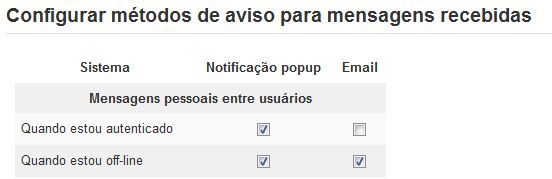
\includegraphics[width=0.6\textwidth]{imagem/cap2/fig12.jpg}}
  \caption{Manipulação das mensagens}
  \label{fig:cap2_12}
 \end{center}
\end{figure}

Entre as opções estão:
\begin{enumerate}
\item Notificações de Atribuição;
\item Notificação de pedido de aprovação de criação de curso;
\item Notificação de rejeição de pedido de criação de curso;
\item Notificação da avaliação do Ensaio;
\item Mensagens pessoais entre usuários;
\item Feedback reminder;
\item Mensagens subscritas do fórum assinados;
\item Notificações de pesquisa.
\end{enumerate}

Além dessas opções, existe como informar outro endereço de e-mail diferente do que está no perfil para receber essas mensagens; e de bloquear o recebimento de mensagens de quem não estiver em seus contatos, mas para isso é necessário a criação de uma lista de contatos, como está illustrado na Figura \ref{fig:cap2_13}.

\begin{figure}[htbp]
 \begin{center}
 \fbox{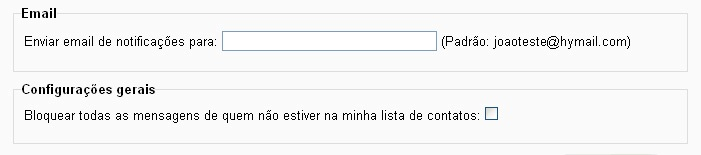
\includegraphics[width=0.6\textwidth]{imagem/cap2/fig13.jpg}}
  \caption{Configuração avançada de mensagem}
  \label{fig:cap2_13}
 \end{center}
\end{figure}

Lembrando que será necessário salvar as modicações no final da página.

\section{Recebendo mensagens}
\index{Recebendo mensagem}
Quando existem mensagens esperando pelo usuário na plataforma, uma pequena janela aparece no canto inferior direito da página inicial, assim que o login é realizado (Figura \ref{fig:cap2_14}).

\begin{figure}[htbp]
 \begin{center}
 \fbox{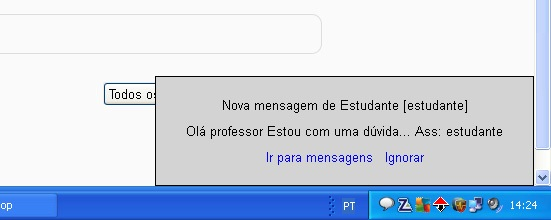
\includegraphics[width=0.4\textwidth]{imagem/cap2/fig14.jpg}}
  \caption{Vizualização do recebimento de novas mensagens}
  \label{fig:cap2_14}
 \end{center}
\end{figure}

Nela haverá links para ler as mensagens, ou para ignorar o aviso.
Ao optar-se por ler as mensagens, uma página com as mensagens ainda não lidas ficará disponível.


 \begin{center}
 \fbox{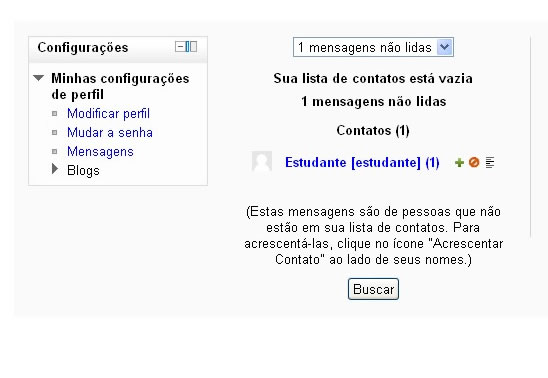
\includegraphics[width=0.4\textwidth]{imagem/cap2/fig15.jpg}}
 \end{center}


Nela é possível clicar em cada mensagem para ler, ou responder. Também existem algumas funcionalidades disponíveis, conforme a Figura abaixo:


 \begin{center}
 \fbox{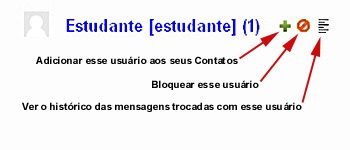
\includegraphics[width=0.4\textwidth]{imagem/cap2/fig16.jpg}}
 \end{center}


Entre as opções estão:

\begin{enumerate}
\item Adicionar aos contatos;
\item Bloquear;
\item Ver histórico.
\end{enumerate}

Ao fazer a opção de ler a mensagem uma tela com o teor da mesma carregará, e se for o caso o usuário poderá la responder (Figura \ref{fig:cap2_17}).

\begin{figure}[!htbp]
 \begin{center}
 \fbox{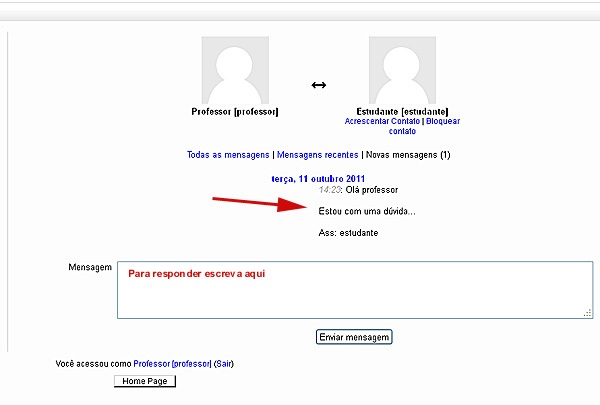
\includegraphics[width=0.3\textwidth]{imagem/cap2/fig17.jpg}}
  \caption{Respondendo a mensagem da disciplina}
  \label{fig:cap2_17}
 \end{center}
\end{figure}

\section{Enviando Mensagens}
\index{Enviando mensagem}
Para enviar uma mensagem para um outro usuário dentro da plataforma Moodle, pode-se ir à \textbf{lista de Participantes} de uma disciplina, clicar no nome escolhido e, em sua página de perfil, clicar em \textbf{Enviar uma Mensagem}, conforme a Figura a seguir.


 \begin{center}
 \fbox{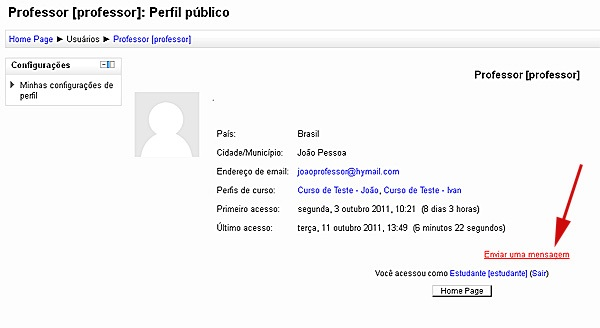
\includegraphics[width=0.4\textwidth]{imagem/cap2/fig18.jpg}}
 \end{center}

Ou ainda, no bloco \textbf{Mensagens} dentro da disciplina, clicar em \textbf{Mensagens} e, na página que abrir, fazer uma busca pelo usuário com quem quer comunicar-se, conforme Figura abaixo:


 \begin{center}
 \fbox{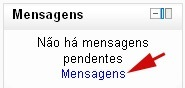
\includegraphics[width=0.3\textwidth]{imagem/cap2/fig19.jpg}}
 \end{center}


Clicando em \textbf{Avançado} pode-se filtrar a busca, conforme as Figuras \ref{fig:cap2_20} e \ref{fig:cap2_21}.

\begin{figure}[htbp]
 \begin{center}
 \fbox{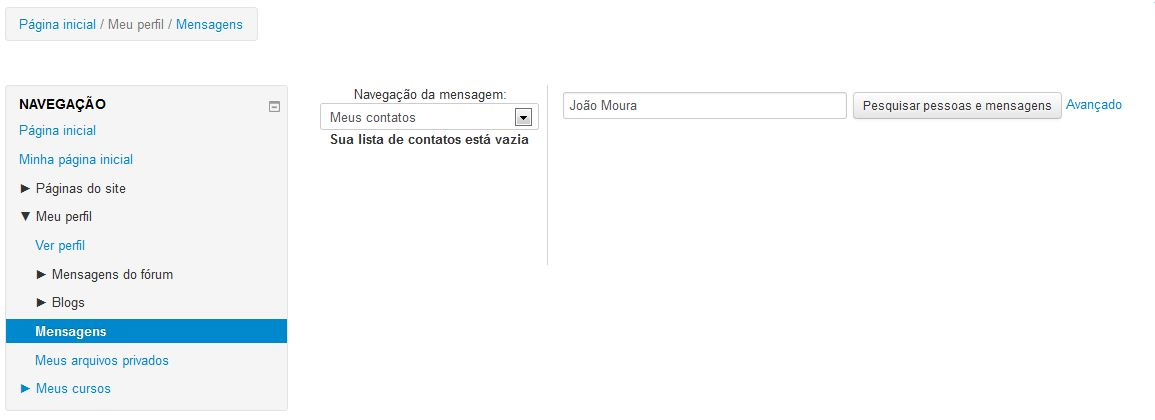
\includegraphics[width=0.5\textwidth]{imagem/cap2/fig20.jpg}}
  \caption{Selecionando usuário para envio de mensagem}
  \label{fig:cap2_20}
 \end{center}
\end{figure}

\begin{figure}[htbp]
 \begin{center}
 \fbox{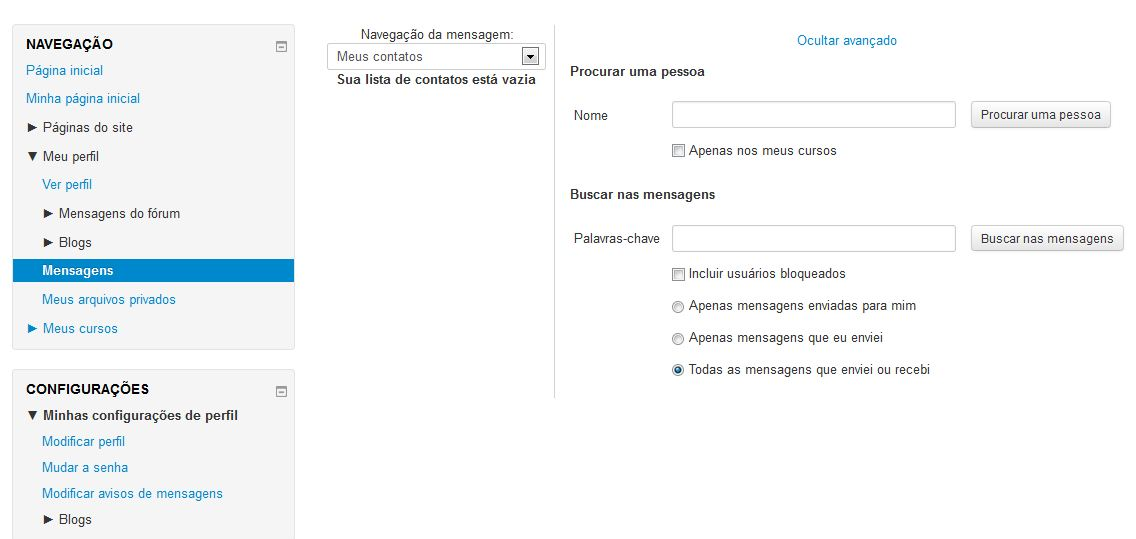
\includegraphics[width=0.5\textwidth]{imagem/cap2/fig21.jpg}}
  \caption{Opções avançadas de envio de mensagem}
  \label{fig:cap2_21}
 \end{center}
\end{figure}


\chapter{Disciplina}
\index{Disciplina}

Neste capítulo serão apresentadas informações importantes para a melhor compreensão e organização da disciplina.

\section{Participante}
\index{Participante}

Ao clicar em \textbf{Participantes}, no bloco \textbf{Participantes da disciplina}, abre-se uma página com a lista de pessoas que estão vinculadas a esta disciplina. Essa lista permite muitos filtros, que tem por objetivo auxiliar o usuário a buscar um aluno, professor ou tutor. 
A Tabela \ref{table:filtrosParticipantes} contém mais detalhes das opções de flitros disponíveis.

\begin{table}[htbp]
\begin{flushleft}
%\begin{wraptable}{t}[5pt]{6cm}
\begin{tabular}{p{6cm}|p{8cm}} \hline
\vspace{0.1cm} 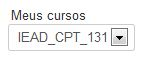
\includegraphics[width=2.2cm]{imagem/cap3/fig1.jpg} & No menu \textbf{Meus cursos} pode-se mudar para a lista de Participantes de outras disciplinas da qual se faça parte.\\ %\hline
\vspace{0.1cm} 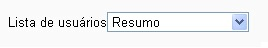
\includegraphics[width=4cm]{imagem/cap3/fig4.jpg}&Em \textbf{Lista de usuários} se escolhe entre uma lista resumida, ou outra mais completa, com mais dados de cada participante.\\%\hline
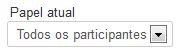
\includegraphics[width=3cm]{imagem/cap3/fig5.jpg}&Papel atual filtra pela função que o participante exerce na disciplina, se é professor, tutor, aluno, etc.\\\hline
\end{tabular}
\caption{Filtros de Participantes}
  \label{table:filtrosParticipantes}
\end{flushleft}
\end{table}%

É possível ordenar uma lista usando o seu cabeçalho como illustra a Figura \ref{fig:cabecalhoLista}.

\begin{figure}[htbp]
 \begin{center}
 \fbox{
\includegraphics[width=0.7\textwidth]{imagem/cap3/fig6.jpg}}
  \caption{Cabeçalho de Listas}
  \label{fig:cabecalhoLista}
 \end{center}
\end{figure}

Ao clicar em um dos cabeçalhos, por exemplo, em \textbf{Nome}, ordena-se a lista segundo o nomes dos participantes. Clicando uma vez, a lista é ordenado em ordem crescente, e clicando mais uma vez, em ordem decrescente.

No topo da lista é possível ver dois menus alfabéticos como na Figura \ref{fig:filtroNomes}. Clicando numa das letras filtra a lista pela letra escolhida, seja \textbf{Nome}, ou \textbf{Sobrenome}. Associando isso ao ordenamento da lista por \textbf{Nome}, por exemplo, tem-se uma ferramenta de grande utilidade.

\begin{figure}[htbp]
 \begin{center}
 \fbox{
\includegraphics[width=0.4\textwidth]{imagem/cap3/fig7.jpg}}
  \caption{Filtro de Nomes}
  \label{fig:filtroNomes}
 \end{center}
\end{figure}

Sem esquecer que, ao clicar-se em cada nome da lista abrirá o perfil público deste.

Outra funcionalidade da \textbf{lista de Participantes} é a que permite enviar mensagens coletivas através da plataforma:
Primeiro filtra-se a lista até obter o grupo com o qual se deseja enviar mensagens. Por exemplo: alunos que não acessam a disciplina há mais de cinco dias.
No inferior da página, clica-se em \textbf{Mostrar todos os \#\#} (onde \#\# é o número de listados após configurar os filtros).
Clica-se então no botão \textbf{Selecionar Tudo}. No menu \textbf{Com os usuários selecionados} escolher \textbf{Enviar uma mensagem} (Veja a Figura \ref{fig:enviarMensagem}).

\begin{figure}[htbp]
 \begin{center}
 \fbox{
\includegraphics[width=0.5\textwidth]{imagem/cap3/fig8.jpg}}
  \caption{Enviar mensagem}
  \label{fig:enviarMensagem}
 \end{center}
\end{figure}
Abrirá uma página com um editor de texto semelhante ao já encontrado em outras partes do Moodle, onde se pode escrever a mensagem. Abaixo desta estará uma lista com os destinatários escolhidos, onde ainda será possível \textbf{Remover} algum que tenha sido colocado inadvertidamente (Veja a Figura \ref{fig:confEnvio}).

\begin{figure}[htbp]
 \begin{center}
 \fbox{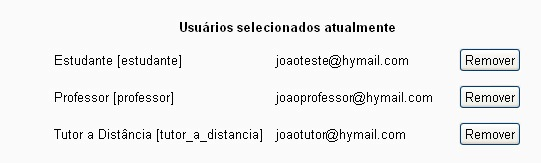
\includegraphics[width=0.7\textwidth]{imagem/cap3/fig9.jpg}}
  \caption{Configurar envio de Mensagens}
  \label{fig:confEnvio}
 \end{center}
\end{figure}

Clica-se em \textbf{Visualização} para ver o texto formatado e, por fim, envia-se a mensagem ou retorna-se para a edição do texto.


\section{Configuração da Disciplina}

Ao clicar no menu Configurações, disponível na página principal da disciplina, dispomos dos recursos descritos na Tabela \ref{tab:32}.


\begin{longtable}[htbp] {p{6cm}|p{9cm}}
  \hline
 \rowcolor[rgb]{0.8,0.8,0.8} \textbf{GERAL} &\\
 \hline
\textbf{Categoria Nome Completo} & Nome da disciplina por extenso. Na UFPB Virtual esse nome segue os padrões do SCA e não pode ser editado por professores ou tutores.\\
\hline

\textbf{Nome breve do curso} & Um nome curto da disciplina, onde se pode ver também o período. Igualmente não é editável, embora visível.\\\hline

\textbf{Número de identificação do curso} & Código da disciplina no SCA. Não pode ser alterado.\\\hline

\textbf{Sumário do curso} & Em um editor de texto pode ser colocada uma descrição breve da disciplina. Essa descrição aparecerá junto ao nome da disciplina na lista de cursos existente na página inicial do Moodle, conforme a figura abaixo:
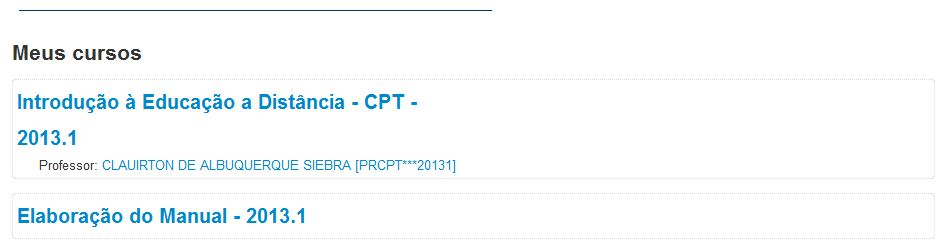
\includegraphics[width=0.6\textwidth]{imagem/cap3/fig25.jpg}\\\hline
\textbf{Formato} & \textbf{Formato Semanal: }
O professor estabelece a data de início e o número de semanas.\\
& \textbf{Formato Tópicos: }
Como no caso do curso semanal, o professor estabelece o número de tópicos e decide quais tópicos ocultar ou não.
Nos formatos Semanal e Tópicos, o Fórum de notícias é criado automaticamente.\\
& \textbf{Formato Social: }
Este formato é articulado em torno de um fórum principal que é publicado na página de abertura do curso. É um formato mais livre que pode ser usado, também, em contextos que não são cursos como, por exemplo, o quadro de avisos de um departamento.\\
& \textbf{Formato Scorm: }
Para se inserir conteúdo no padrão Scorm pode-se adicionar um recurso nesse padrão, ou criar uma disciplina em FORMATO SCORM. Essa opção é para usuários avançados, que tem conhecimento deste padrão e das ferramentas que o geram.
\\\hline
\textbf{Número de semanas ou tópicos} & Escolhe-se o número de semanas ou tópicos que a disciplina durará. Esse campo, aliado à data de início do curso, determinará as datas de cada semana, que o Moodle coloca automaticamente.\\\hline
\textbf{Data de início do curso} & Data do início do curso\\\hline
\textbf{Seções escondidas} & \textbf{Seções escondidas são mostradas contraídas:} significa que aquela semana ou tópico que for tornada oculta será mostrado ao estudante, porém com uma advertência: “não disponível”, não podendo ser acessada.\\
& \textbf{Seções escondidas são completamente invisíveis:} significa que o aluno não vê nada no lugar daquela semana ou tópico.
\\\hline
\textbf{Quantas notícias quer mostrar} & Esta configuração define o número de notícias recentes que serão visualizadas na página principal do curso, no bloco "Últimas Notícias".
Se você definir o valor como "0 itens" o bloco "Últimas Notícias" não será visualizado.
\\\hline
\textbf{Mostrar livro de notas aos estudantes} & Permite ou não a visualização do Quadro de Notas pelos alunos.\\\hline
\textbf{Mostrar relatório das atividades} & O relatório das atividades de cada usuário mostra todas as atividades daquele usuário no curso atual. Este relatório contém uma lista de todas as atividades realizadas e das mensagens individuais. Além disto, contém um arquivo detalhado de todos os acessos do usuário ao curso.
Os professores têm acesso constante a este relatório, que é disponível na página do perfil de cada usuário.
Escolhendo \textbf{SIM} ou \textbf{NÃO} é possível escolher a opção de mostrar, ou não, estes dados aos alunos.
\\\hline
\textbf{Tamanho máximo de upload} & O tamanho máximo de cada arquivo enviado para o site é definido para o Moodle inteiro pelo administrador da plataforma. Normalmente esse limite é definido também nas configurações do servidor.
Porém o professor pode, na sua disciplina, definir um valor menor do que o limite geral, escolhendo dentre os valores apresentados.\\\hline
%%%%%%%%%%%%%%%%%%%%%%%%%%%%%%%%%%%%%%%%%%%%%%%%%%%%%%%%%%%%%%%%%%%%%%%%%%%%%%%%%%%%%%%%%%%%%%%%%%%%%%%%%%%%%
\rowcolor[rgb]{0.8,0.8,0.8} \textbf{ACESSO COMO VISITANTE}&\\\hline
\textbf{Permitir o acesso de visitantes} & Visitantes são usuários não autenticados, ou que não fizeram login, aos quais é permitida uma visita à plataforma, sem permissão para participar ou alterar nada. Pode-se permitir, ou não, o acesso de visitantes a uma disciplina, sem que precisem estar matriculados na mesma.\\\hline
\textbf{Senha} & No caso de se permitir visitantes à disciplina, é possível criar uma senha para restringir o acesso a quem conheça a chave.\\\hline
\rowcolor[rgb]{0.8,0.8,0.8} \textbf{GRUPOS}&\\\hline
\textbf{Modalidade grupo} & Esta configuração possui três opções:\\
&\textbf{Nenhum grupo} - Não há subgrupos, todos fazem parte de uma grande comunidade;\\
&\textbf{Grupos separados} - Cada membro de grupo pode ver apenas seu próprio grupo, os outros são invisíveis;\\
&\textbf{Grupos visíveis} - Cada membro do grupo trabalha no seu próprio grupo, mas pode também ver outros grupos;
O tipo de grupo definido no nível da disciplina é o padrão para todas as atividades do curso. Cada atividade que suporta grupos pode também definir seu próprio tipo de grupo.
\\\hline
\textbf{Forçar modalidade grupo}& Se o modo de grupo é forçado, então o modo de grupo é aplicado a todas as atividades da disciplina. Configurações do modo de grupo de cada atividade serão ignoradas.\\\hline
\textbf{Agrupamento padrão} & Nas configurações de grupos da disciplina, clicando na aba Agrupamentos, é possível criar agrupamentos de grupos, que aparecerão nesta opção para escolha do agrupamento padrão. Se não houver agrupamentos somente haverá a opção Nenhum.\\\hline
%%%%%%%%%%%%%%%%%%%%%%%%%%%%%%%%%%%%%%%%%%%%%%%%%%%%%%%%%%%%%%%%%%%%%%%%%%%%%%%%%%%%%%%%%%%%%%%%%%%%%%%%%%%%%
\rowcolor[rgb]{0.8,0.8,0.8} \textbf{DISPONIBILIDADE}&\\\hline
\textbf{Disponibilidade }& A opção \textbf{Esse curso pode ser acessado pelos participantes} é o padrão. Escolhendo a opção \textbf{Esse curso não pode ser acessado pelos participantes}, a disciplina fica oculta.\\\hline

%%%%%%%%%%%%%%%%%%%%%%%%%%%%%%%%%%%%%%%%%%%%%%%%%%%%%%%%%%%%%%%%%%%%%%%%%%%%%%%%%%%%%%%%%%%%%%%%%%%%%%%%%%%%%
\rowcolor[rgb]{0.8,0.8,0.8} \textbf{IDIOMA}&\\\hline
\textbf{Forçar língua} & O padrão é \textbf{NÃO FORÇAR}. Pode-se optar por forçar alguns dos idiomas disponíveis, como por exemplo: Português - Brasil (pt\_br). Nesse caso a mudança de idioma na plataforma não surtirá efeito na disciplina.\\\hline

%%%%%%%%%%%%%%%%%%%%%%%%%%%%%%%%%%%%%%%%%%%%%%%%%%%%%%%%%%%%%%%%%%%%%%%%%%%%%%%%%%%%%%%%%%%%%%%%%%%%%%%%%%%%%
\rowcolor[rgb]{0.8,0.8,0.8} \textbf{RENOMEAR PAPEL (FUNÇÃO)}&\\\hline
 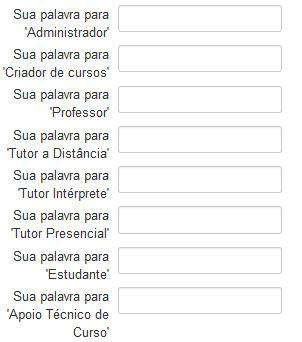
\includegraphics[width=4cm]{imagem/cap3/fig10.jpg} & As principais funções presentes na disciplina podem ser renomeadas. Isso fará com que sejam apresentadas com o novo nome em determinados locais dentro da disciplina, como quando se filtra os Participantes por sua função (papel atual), etc.
Ao clicar-se em Mostrar Avançado, ao lado deste quadro, algumas outras funções serão acrescentadas a lista para renomear.\\\hline

\includegraphics[width=3cm]{imagem/cap3/fig11.jpg} & Ao terminar de configurar a disciplina deve-se SALVAR.\\\hline
\caption{Itens de Configuração da Disciplina}
\label{tab:32}
\end{longtable}

\section{Configurações/Filtros}
Ao selecionar o item \textbf{Filtros no bloco Configurações}, dentro de uma disciplina, pode-se habilitar ou desabilitar os filtros presentes na plataforma (Veja a Figura \ref{Fig: filtroConf}).
\begin{figure}[htbp]
 \begin{center}
 \fbox{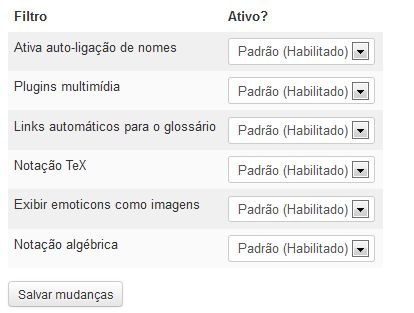
\includegraphics[width=0.4\textwidth]{imagem/cap3/fig12.jpg}}
  \caption{Filtro do bloco de Configurações}
  \label{Fig: filtroConf}
 \end{center}
\end{figure}
As mudanças feitas aqui serão válidas somente dentro da disciplina.

\section{Configurações/BackUp}
Ao clicar-se em \textbf{Backup} tem início uma sequência de páginas com os passos de configuração para se obter uma cópia da disciplina para uma futura restauração (Veja Figura \ref{Fig: confBackup}).

\begin{figure}[htbp]
 \begin{center}
 \fbox{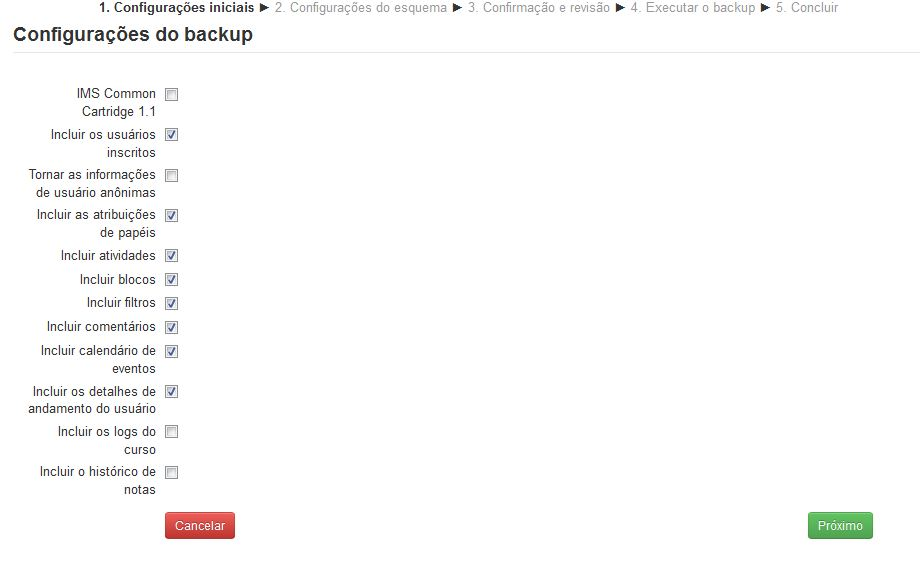
\includegraphics[width=0.8\textwidth]{imagem/cap3/fig13.jpg}}
  \caption{Configuração do Backup}
  \label{Fig: confBackup}
 \end{center}
\end{figure}

Na primeira tela escolhem-se os itens que irão fazer parte do backup. Dependendo das permissões de cada usuário alguns desses itens não farão parte da cópia obtida, ou não permitirão opção de escolha. Na Figura~\ref{Fig: confBackup}, na configuração padrão do Moodle para professores, somente os itens “Incluir Atividades”, “Incluir blocos” e “Incluir filtros” permitem escolha. Ao término, clica-se em \textbf{Próximo}.

A segunda tela, illustrada na Figura \ref{Fig: sentAtiv}), nos traz as \textbf{Semanas e as Atividades}, uma a uma, com a opção de selecionar ou não, para o caso de querermos um backup de somente alguns tipos de atividades, por exemplo, ou de somente uma semana, ou tópico. E assim por diante. Ao final, clica-se em \textbf{Próximo}.

\begin{figure}[htbp]
 \begin{center}
 \fbox{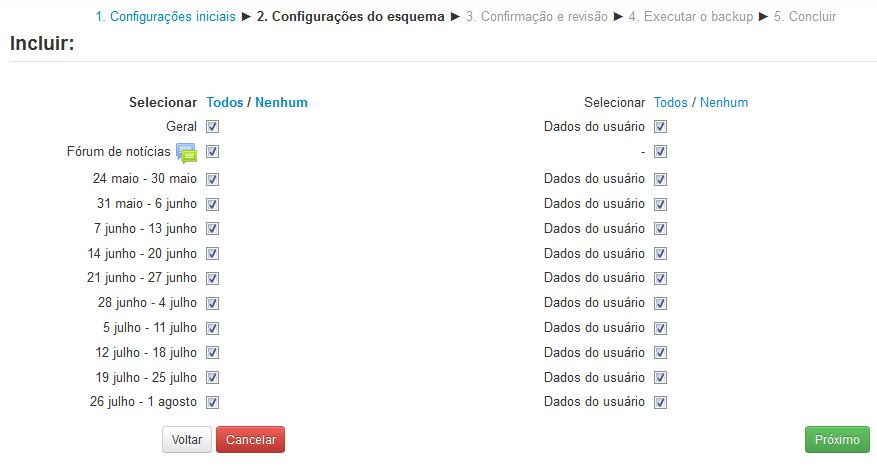
\includegraphics[width=0.6\textwidth]{imagem/cap3/fig14.jpg}}
  \caption{Semanas e atividades}
  \label{Fig: sentAtiv}
 \end{center}
\end{figure}

Após esse passo é mostrada uma lista das opções feitas para verificação. É também possível nomear o arquivo ZIP que será gerado (Veja a Figura \ref{Fig: envioBackup}).

\begin{figure}[htbp]
 \begin{center}
 \fbox{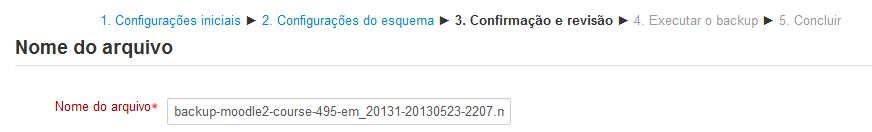
\includegraphics[width=0.6\textwidth]{imagem/cap3/fig15.jpg}}
  \caption{Envio de Backup}
  \label{Fig: envioBackup}
 \end{center}
\end{figure}

Tendo conferido todas as opções selecionadas e dados inserigos, clica-se em \textbf{Executar o Backup} para iniciar o processo de cópia. É necessário esperar alguns instantes, dependendo da quantidade de conteúdos da disciplina e das escolhas feitas previamente. Ao finalizar o processamento do backup aparecerá uma mensagem parecida a aquela na Figura \ref{Fig: confEnvio}.

\begin{figure}[htbp]
 \begin{center}
 \fbox{
\includegraphics[width=0.6\textwidth]{imagem/cap3/fig16.jpg}}
  \caption{Confirmação de Envio}
  \label{Fig: confEnvio}
 \end{center}
\end{figure}
Clicando-se em \textbf{Continuar abre uma listagem de Backups} (Veja a Figura \ref{Fig: genrecBackup}), onde se pode restaurar o arquivo gerado (\textcolor{blue}{Restaurar}), baixar para o computador do usuário (\textcolor{blue}{Download}), ao lado de cada arquivo da lista e gerenciar os arquivos existentes, e clicando no botão \textbf{Gerenciar os arquivos de backup}, outras funcionalidade podem ser usadas.
\begin{figure}[htbp]
 \begin{center}
 \fbox{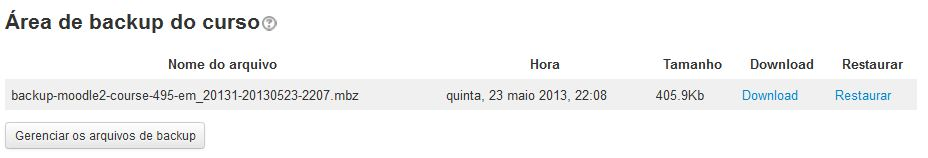
\includegraphics[width=0.7\textwidth]{imagem/cap3/fig17.jpg}}
  \caption{Gerenciar Backups}
  \label{Fig: genrecBackup}
 \end{center}
\end{figure}

Essas funcionalidades extras ao gerenciar os arquivos de backup, podem ser vistas na Figura \ref{Fig: genrecExtraBackup}. Pode-se acrescentar arquivos, tanto originados de outro diretório no servidor, quanto do computador do usuário, pode-se baixar os arquivos existentes em lote (todos), e ao clicar ao lado do nome do arquivo aparece um menu de contexto ligado a este, que permite baixá-lo, mudar o nome, mover e excluir (se o formato for .zip aparece também a funcionalidade \textbf{Descompactar}).

\begin{figure}[htbp]
 \begin{center}
 \fbox{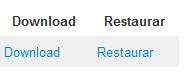
\includegraphics[width=0.3\textwidth]{imagem/cap3/fig18.jpg}}
  \caption{Funcionalidades Extras na Gerencia dos Backups}
  \label{Fig: genrecExtraBackup}
 \end{center}
\end{figure}

\section{Configurações/Restaurar}
\label{chap3:sec:restaurar}
Ao se escolher \textbf{Restaurar}, no bloco \textbf{Configurações} de uma disciplina, abrirá a mesma página que aparece ao fim do backup (Veja a Figura \ref{Fig: genrecBackup}).
As mesmas informações descritas acima também cabem aqui integralmente.
Ao clicar em \textcolor{blue}{Restaurar} uma sequência de sete passos é iniciada. A cada um é possível voltar ao anterior, ou avançar.

\begin{enumerate}
 \item \textbf{Confirmar:} informações sobre o backup, com a versão do moodle, formato, etc.; sobre a configuração do backup realizado quando da criação do arquivo; os detalhes do curso, suas seções e atividades, são listadas. Todas as informações são somente para conferência, não permitindo mudanças.
 
 \item \textbf{Destino:} nesta etapa decide-se se:
esse conteúdo será acrescentado ao já existente, ou
se o conteúdo do arquivo de backup sobreporá o conteúdo existente na disciplina.

\item \textbf{Configurações:} algumas configurações do backup são agora apresentadas na restauração, permitindo que se mantenha, ou se retire certos itens.

\item \textbf{Esquema:} uma lista de todas as seções (semanas ou tópicos) e atividades disciplinares presentes no backup. É possível desmarcar uma ou mais seções e atividades, caso seja do interesse restaurar somente algumas e não outras. É possível também renomear a disciplina, assim como escolher se as seções do backup sobreporão as já existentes na disciplina.

\item \textbf{Revisar:} todas as configurações e conteúdo escolhido são listados novamente, para conferência. Caso tudo esteja dentro do esperado, clica-se no botão \textbf{Executar a Restauração} para iniciar o \textbf{Processamento} do pedido de restauração. 
Após um breve período de tempo, dependendo do tamanho do backup, o processo concluí com uma mensagem parecida com aquela na 
Figura \ref{Fig: fim}.
\end{enumerate}

Ao clicar no botão Continuar abre novamente a página da disciplina, já restaurada.


\begin{figure}[htbp]
 \begin{center}
 \fbox{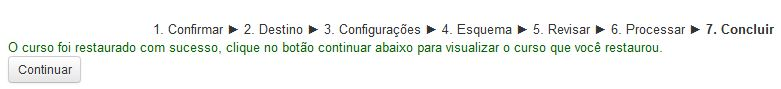
\includegraphics[width=0.8\textwidth]{imagem/cap3/fig19.jpg}}
  \caption{Conclusão do Processo de Configuração/Restauração}
  \label{Fig: fim}
 \end{center}
\end{figure}


\section{Configurações/Importar}
Essa é uma funcionalidade semelhante à restauração de backup. Porém ao invés de se usar um arquivo, pode-se importar diretamente de outra disciplina existente na mesma plataforma.

Cabe aqui explicar que o nível de permissão do usuário afetará diretamente a importação. Um professor, por exemplo,  poderá somente importar as suas próprias disciplinas, ou melhor, as disciplinas onde seja titular. É uma função útil pois permite importar o conteúdo de uma disciplina dada em um período anterior (Veja a Figura \ref{Fig: cap3_20}).

\begin{figure}[htbp]
 \begin{center}
 \fbox{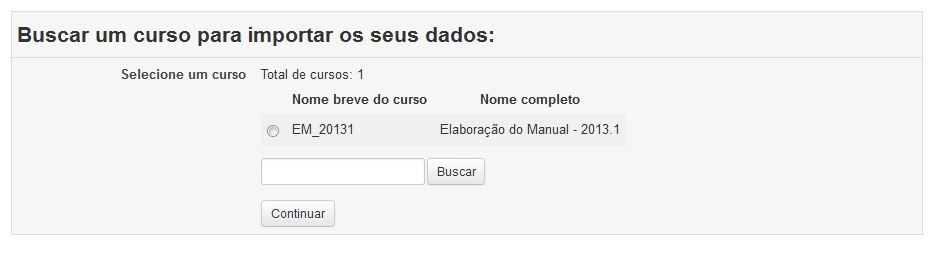
\includegraphics[width=0.7\textwidth]{imagem/cap3/fig20.jpg}}
  \caption{Importação de Dados}
  \label{Fig: cap3_20}
 \end{center}
\end{figure}

Ao escolher uma disciplina a ser importada, clica-se em \textbf{Continuar}. Novamente teremos a execução das etapas descritas na Seção~\ref{chap3:sec:restaurar} (Veja a Figura \ref{Fig: cap3_21}).
Em \textbf{Configurações iniciais} pode-se retirar ou manter algumas configurações da disciplina a ser importada, conforme a imagem 
na Figura \ref{Fig: cap3_21}.

\begin{figure}[htbp]
 \begin{center}
 \fbox{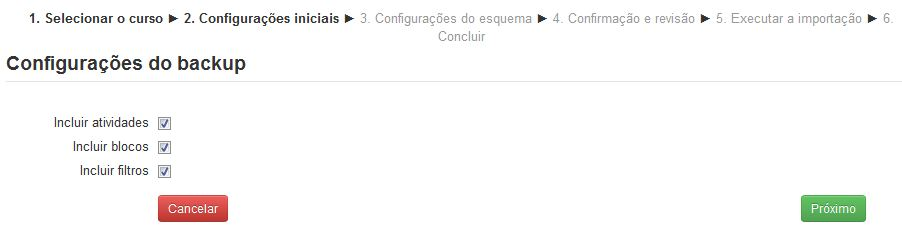
\includegraphics[width=0.8\textwidth]{imagem/cap3/fig21.jpg}}
  \caption{Importação de Disciplina}
  \label{Fig: cap3_21}
 \end{center}
\end{figure}



O terceiro passo, \textbf{Configurações do esquema} (Fig. \ref{Fig: cap3_22}), permite a escolha de certas semanas (ou tópicos) e das atividades e recursos que se quer importar.

\begin{figure}[htbp]
 \begin{center}
 \fbox{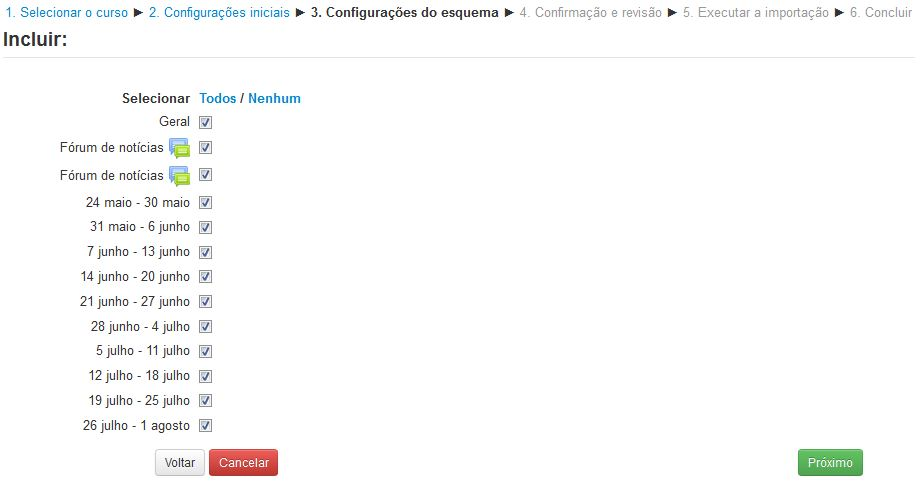
\includegraphics[width=0.7\textwidth]{imagem/cap3/fig22.jpg}}
  \caption{Configuração de Esquema}
  \label{Fig: cap3_22}
 \end{center}
\end{figure}

A quarta etapa, \textbf{Confirmação e revisão}, listará as escolhas feitas. Lembrando que sempre é possível voltar às etapas anteriores. Após conferir os dados inseridos, clica-se no botão \textbf{Executar a importação}.

Ao final de alguns instantes, enquanto o sistema executa a importação, chega-se a etapa final, \textbf{Concluir}, com a apresentação da mensagem 
na Figura~\ref{Fig: cap3_23}.

\begin{figure}[htbp]
 \begin{center}
 \fbox{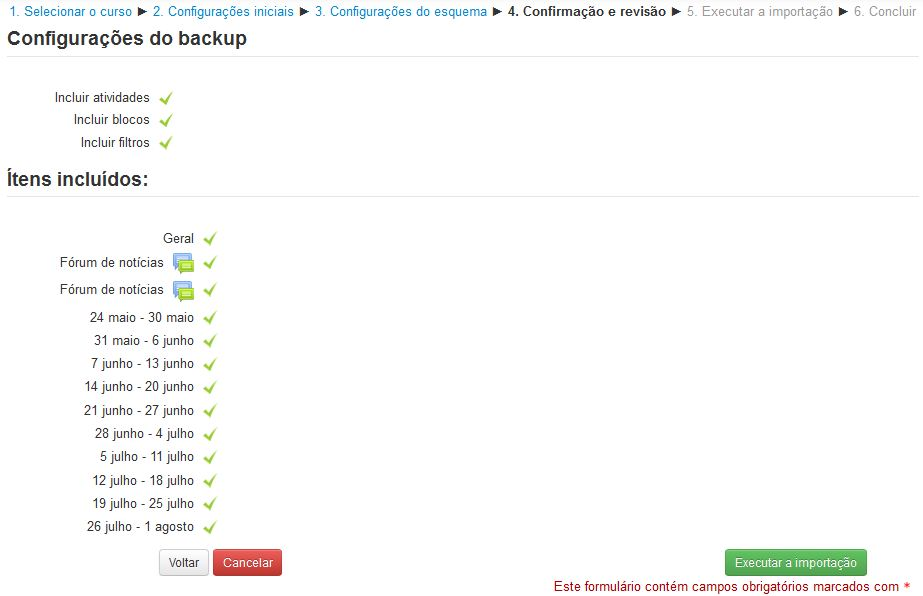
\includegraphics[width=0.6\textwidth]{imagem/cap3/fig23.jpg}}
  \caption{Configuração de Esquema}
  \label{Fig: cap3_23}
 \end{center}
\end{figure}

\section{Configurações/Reconfigurar (course/reset)}
Esta página permite que você esvazie os dados de uma disciplina, sem excluir as atividades e outras configurações (Conforme a Tabela \ref{tab:Conf3}), no caso de eventual reaproveitamento para outro período. As exclusões não poderão ser revertidas.

\begin{longtable}[htbp!]{p{6cm}|p{9cm}}
\hline
%%%%%%%%%%%%%%%%%%%%%%%%%%%%%%%%%%%%%%%%%%%%%%%%%%%%%%%%%%%%%%%%%%%%%%%%%%%%%%%%%%%%%%%%%%%%%%%%%%%%%%%%%%%%%
\rowcolor[rgb]{0.8,0.8,0.8} \textbf{GERAL}&\\\hline
\textbf{Data de início do curso} & Esta configuração determina o início da primeira semana para um curso em formato semanal. Também determina a data inicial em que os logs das atividades do curso estarão disponíveis. No caso de atividades herdadas da antiga disciplina, ou já existentes, o Moodle reconfigura a data de início e fim da atividade, em função da semana onde está inserida.\\\hline
\textbf{Excluir eventos} & Seleciona-se caso queira excluir todos os eventos da disciplina\\\hline
\textbf{Excluir logs} & Seleciona-se para excluir todos os logs da disciplina.\\\hline
\textbf{Excluir todas as anotações} & Seleciona-se para excluir todas as anotações na disciplina.\\\hline
\textbf{Excluir todos os comentários} & Seleciona-se para excluir todos os comentários (feedbacks) da disciplina.\\\hline
\textbf{Excluir dados de conclusão de curso} & Seleciona-se para excluir todos os dados de conclusão de curso da disciplina.\\\hline
\textbf{Apagar de associações de blog} & Se selecionado, as mensagens do blog não serão mais associadas a esta disciplina ou a atividades ou recursos da disciplina. As mensagens não serão apagadas.\\\hline
%%%%%%%%%%%%%%%%%%%%%%%%%%%%%%%%%%%%%%%%%%%%%%%%%%%%%%%%%%%%%%%%%%%%%%%%%%%%%%%%%%%%%%%%%%%%%%%%%%%%%%%%%%%%%
\rowcolor[rgb]{0.8,0.8,0.8} \textbf{FUNÇÕES}&\\\hline
\textbf{Cancelar inscrições} & Marcam-se as funções que se quer cancelar, como tutores, ou estudantes. Pode-se pressionar a tecla Ctrl para selecionar mais de uma função.\\\hline
\textbf{Excluir todas as sobreposições no curso \textcolor{blue}{$\ast$}} & Ao marcar-se essa opção todas as permissões de usuário que tenham sido modificadas somente dentro da disciplina, voltarão ao padrão da plataforma.\\\hline
\textbf{Excluir todas as designações de funções locais} & O mesmo que Cancelar inscrições, porém equivale a marcar todas as funções existentes.\\\hline
%%%%%%%%%%%%%%%%%%%%%%%%%%%%%%%%%%%%%%%%%%%%%%%%%%%%%%%%%%%%%%%%%%%%%%%%%%%%%%%%%%%%%%%%%%%%%%%%%%%%%%%%%%%%%
\rowcolor[rgb]{0.8,0.8,0.8} \textbf{LIVRO DE NOTAS}&\\\hline
\textbf{Remova todos os itens e categorias} & Seleciona-se para excluir, no Quadro de Notas da disciplina, todos os itens de nota e categorias que tenham sido criados até então.\\\hline
\textbf{Remova todas as notas} & Ao selecionar-se essa opção todas as notas na disciplina serão excluídas.\\\hline
%%%%%%%%%%%%%%%%%%%%%%%%%%%%%%%%%%%%%%%%%%%%%%%%%%%%%%%%%%%%%%%%%%%%%%%%%%%%%%%%%%%%%%%%%%%%%%%%%%%%%%%%%%%%%
\rowcolor[rgb]{0.8,0.8,0.8} \textbf{GRUPOS}&\\\hline
\textbf{Excluir todos os grupos \textcolor{blue}{$\ast$}} & Exclui todos os grupos criados na disciplina. Note que os pólos são grupos e, eventualmente, não devem ser apagados.\\\hline
\textbf{Remover todos os membros do grupo \textcolor{blue}{$\ast$}} & Retira os membros de cada grupo, mantendo os grupos.\\\hline
\textbf{Excluir todos os agrupamentos \textcolor{blue}{$\ast$}} & Os agrupamentos são grupos de grupos. Essa opção, se marcada, reconfigurará a disciplina sem os agrupamentos existentes.\\\hline
\textbf{Remover todos os grupos dos agrupamentos \textcolor{blue}{$\ast$}} & Ao marcar-se essa opção todos os grupos do agrupamento serão removidos.\\\hline
%%%%%%%%%%%%%%%%%%%%%%%%%%%%%%%%%%%%%%%%%%%%%%%%%%%%%%%%%%%%%%%%%%%%%%%%%%%%%%%%%%%%%%%%%%%%%%%%%%%%%%%%%%%%%
\rowcolor[rgb]{0.8,0.8,0.8} \textbf{TAREFAS}&\\\hline
\textbf{Excluir todos os arquivos enviados} & Exclui os arquivos enviados nas atividades existentes da disciplina.\\\hline
%%%%%%%%%%%%%%%%%%%%%%%%%%%%%%%%%%%%%%%%%%%%%%%%%%%%%%%%%%%%%%%%%%%%%%%%%%%%%%%%%%%%%%%%%%%%%%%%%%%%%%%%%%%%%
\rowcolor[rgb]{0.8,0.8,0.8} \textbf{CHATS}&\\\hline
\textbf{Remover todas as mensagens} & Exclui todas as mensagens dos bate-papos (chats) existentes na disciplina.\\\hline
%%%%%%%%%%%%%%%%%%%%%%%%%%%%%%%%%%%%%%%%%%%%%%%%%%%%%%%%%%%%%%%%%%%%%%%%%%%%%%%%%%%%%%%%%%%%%%%%%%%%%%%%%%%%%
\rowcolor[rgb]{0.8,0.8,0.8} \textbf{FÓRUNS}&\\\hline
\textbf{Excluir todas as mensagens} & Exclui todas as mensagens de todos os fóruns da disciplina.\\\hline
\textbf{Excluir as mensagens de \textcolor{blue}{$\ast$}} & Exclui as mensagens dos fóruns filtrados por tipo de fórum.
Ex: fórum geral, fórum de notícias, etc.\\\hline
\textbf{Excluir todas as subscrições \textcolor{blue}{$\ast$}} & Aqui subscrição é usada para quando um usuário se torna assinante de um fórum. Ao se tornar assinante, ele passa a receber as mensagens desse fórum por e-mail. Selecionando esse item essas subscrições são excluídas.\\\hline
\textbf{Excluir todas as preferências de rastreamento dos fóruns \textcolor{blue}{$\ast$}} & Ao subscrever um fórum o usuário pode escolher se receberá por email, ou outras preferências. Ao se marcar esse item essas preferências serão excluídas. \\\hline
\textbf{Excluir todas as pontuações} & Exclui todos os pontos dados às participações nos fóruns desta disciplina.\\\hline
\caption{Descrição das opções de configuração e re-configuração de disciplinas.}
  \label{tab:Conf3}
\end{longtable}
(\textcolor{blue}{$\ast$})Esta é uma opção avançada e pode ser acessada somente se o botão \textbf{Mostrar Avançado} for clicado.

Na parte de baixo da página de reconfiguração há quatro botões, os quais dois são descritos na Figura \ref{fig:cap3_24}, enquanto 
que os botões \textbf{Desmarcar todas as seleções} e \textbf{Cancelar} são auto-explicativos.

\begin{figure}[htbp]
 \begin{center}
 \fbox{
\includegraphics[width=0.5\textwidth]{imagem/cap3/fig24.jpg}}
  \caption{Configurações da Disciplina}
  \label{fig:cap3_24}
 \end{center}
\end{figure}

\chapter{Recursos: como criar e configurar}

\section{Conteúdo do pacote IMS}

IMS Global Learning Consortium, ou simplesmente IMS, refere-se a um consórcio entre instituições de ensino, editoras, empresas do setor tecnológico, organizações governamentais e iniciativas regionais que se organizaram com intuito de apoiar o uso da tecnologia como forma de transformar a aprendizagem educacional (CONSORTIUM, 2011).

Um pacote IMS refere-se a uma estrutura de arquivos criados sob as especificações do padrão \emph{IMS Content Packaging}. Pacotes IMS permitem a exportação e importação de conteúdo de um ambiente virtual de aprendizado para outro, indicando seu reaproveitamento (SPECIFICATION, 2011).

Muitos softwares permitem a exportação de seu conteúdo por meio de pacotes IMS, entre eles pode-se citar o
ExeLearning (\url{http://exelearning.org}) e o Reload (\url{http://www.reload.ac.uk}).

Apesar de sua grande utilidade e funcionalidade, este recurso ainda é pouco explorado devido a alguns problemas ocorridos no reaproveitamento de conteúdo entre versões distintas de ambientes virtuais de aprendizagem (SILVA, 2010). 

\subsection{Acrescentando o recurso Conteúdo do pacote IMS}

Para acrescentar o recurso Conteúdo do pacote IMS deve-se:
\begin{enumerate}
\item Na disciplina desejada, clicar no botão \textbf{Ativar edição};
\item Primeiro deve-se clicar na opção \textbf{Adicionar uma atividade ou recurso}, e só então aparecerá a opção de \textbf{Acrescentar}. Em seguida, basta escolher a opção \textbf{Conteúdo od pacote IMS} na lista \textbf{Recursos} e clicar em \textbf{Acrescentar};
\item No formulário apresentado, preencher obrigatoriamente os campos \textbf{Nome} (nome do recurso que ficará visível na plataforma) e \textbf{Descrição} (informações gerais sobre o recurso);
\item Clicar no botão  \textbf{Escolher um arquivo}  selecionar o pacote IMS e enviá-lo.
\end{enumerate}

Alguns softwares oferecem a possibilidade de unir vários pacotes IMS em apenas um. Se esse for o caso, na opção \textbf{Arquivos de pacote}, selecionar a quantidade de pacotes que foram unidos;

Na opção \textbf{Visível}, informar se o recurso ficará disponível ou oculto para os alunos;
caso necessário, preencher o campo \textbf{Número de identificação do módulo} para fins de cálculo de avaliação.

Salvar as configurações realizadas clicando no botão \textbf{Salvar e voltar ao curso}  para salvar e retornar para a disciplina ou no botão \textbf{Salvar e mostrar }para salvar e mostrar o recurso criado.

\section{Página}

O Recurso página, illutrada na Figura \ref{fig:cap4_1}, é um recurso muito utilizado no Moodle, pois possui inúmeras finalidades. Ela pode ser utilizada para disponibilizar avisos, ementas, cronogramas, horários, álbum de fotos, videoteca, lista de links, lista de endereços de contato, entre outras possibilidades. Além disso, o recurso página segue os mesmos princípios de edição do \textit{HyperText Markup Language }(HTML).
\begin{figure}[htbp]
 \begin{center}
 \fbox{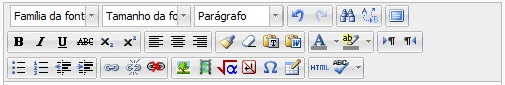
\includegraphics[width=0.6\textwidth]{imagem/cap4/fig1.jpg}}
  \caption{Página}
  \label{fig:cap4_1}
 \end{center}
\end{figure}
A semelhança com o editor de texto Word da Microsoft\footnote{Empresa multinacional de tecnologia e informática} também facilita a construção deste recurso. A seguir apresenta-se o menu de formatação e edição de textos do Moodle.

Este menu é comum a diversos recursos e atividades, suas opções são listadas na Tabela \ref{table:cap4_table1}.

\begin{table}[htbp]
\begin{flushleft}
\begin{tabular}{p{8cm}|p{6cm}} \hline
\rowcolor[rgb]{0.8,0.8,0.8} \textbf{Ícone}& \textbf{Descrição}\\\hline
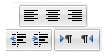
\includegraphics[width=0.1\textwidth]{imagem/cap4/fig2.jpg} & Alinhamento e posicionamento do texto \\\hline

\includegraphics[width=0.07\textwidth]{imagem/cap4/fig3.jpg} & Inserção, remoção e impedimento de links \\\hline
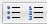
\includegraphics[width=0.08\textwidth]{imagem/cap4/fig4.jpg} & Marcadores e numeração \\\hline

\includegraphics[width=0.15\textwidth]{imagem/cap4/fig5.jpg} & Inserção de imagem, vídeo, equação, caracteres especiais, espaço em branco e tabela\\\hline
\includegraphics[width=0.09\textwidth]{imagem/cap4/fig6.jpg} & Definição de cores\\\hline
\includegraphics[width=0.09\textwidth]{imagem/cap4/fig7.jpg} & Editor de linguagem HTML\\\hline
\includegraphics[width=0.13\textwidth]{imagem/cap4/fig8.jpg} & Remoção de código incorreto e formatação, colagem de textos\\\hline
\includegraphics[width=0.08\textwidth]{imagem/cap4/fig9.jpg} & Corretor ortográfico\\\hline
\includegraphics[width=0.25\textwidth]{imagem/cap4/fig10.jpg} & Definição do tipo e tamanho da fonte, parágrafo e outras características gerais do texto\\\hline
\includegraphics[width=0.25\textwidth]{imagem/cap4/fig11.jpg} & Desfazer (CTRL+Z), refazer (CTRL+Y), localizar/substituir, tela inteira.\\\hline
\end{tabular}
\caption{Configurações de Página}
  \label{table:cap4_table1}
\end{flushleft}
\end{table}%

Aconselha-se que cada funcionalidade do editor de texto seja testada pelo usuário, já que a manipulação correta dos recursos do editor pode facilitar e agilizar a construção de um texto. A função de cada item do editor é exibida toda a vez que se posiciona o ponteiro do mouse sobre cada ícone.

\subsection{Acrescentando o recurso página}

Para acrescentar o recurso Página deve-se seguir os passos abaixo:
\begin{enumerate}
\item Na disciplina desejada, clicar no botão \textbf{ Ativar edição};
\item Primeiro deve-se clicar na opção \textbf{Adicionar uma atividade ou recurso}, e só então aparecerá a opção de \textbf{Acrescentar}. Em seguida basta escolher a opção \textbf{Página} na lista \textbf{Recursos} e clicar em \textbf{Acrescentar};
\item No formulário apresentado, preencher obrigatoriamente os campos \textbf{Nome} (nome do recurso que ficará visível na plataforma) e \textbf{Descrição} (informações gerais sobre o recurso);
\item O campo \textbf{conteúdo da página}, como o próprio nome sugere, é responsável por aquilo que será exibido para o usuário. Este campo também é de preenchimento obrigatório;
\item Caso seja necessário, marcar a caixa de seleção \textbf{mostrar o nome da página}. Ela é responsável por exibir o nome da página após o clique do usuário no recurso página;
\item Caso seja necessário, marcar a caixa de seleção \textbf{exibir descrição da página}. Ela é responsável por exibir o conteúdo preenchido no campo descrição da página, após o clique do usuário neste recurso;
\item Na opção \textbf{Visível}, informar se o recurso ficará disponível ou oculto para os alunos;
\item Caso seja necessário, preencher o campo \textbf{Número de identificação do módulo} para fins de cálculo de avaliação.
\item Salvar as configurações realizadas clicando no botão  \textbf{Salvar e voltar ao curso} para salvar e retornar para a disciplina ou no botão \textbf{Salvar e mostrar } para salvar e exibir a página criada.
\end{enumerate}

\subsection{Inserindo uma imagem em uma página}

Para inserir uma imagem em uma página, deve-se clicar no ícone: \includegraphics{imagem/cap4/fig12.jpg}. Uma janela, como aquela illustrada na Figura \ref{fig:cap4_13}, será exibida. Basta então clicar em \textbf{Encontrar} ou enviar uma imagem para poder selecionar a imagem que se deseja
adcionar a uma página.

\begin{figure}[htbp]
 \begin{center}
 \fbox{\includegraphics[width=0.5\textwidth]{imagem/cap4/fig13.jpg}}
  \caption{Enviando Imagem}
  \label{fig:cap4_13}
 \end{center}
\end{figure}

Na próxima janela exibida (Figura \ref{fig:cap4_14}), clicar em \textbf{Enviar um arquivo} e em seguida em \textbf{Escolher um arquivo}.
\begin{figure}[htbp]
 \begin{center}
 \fbox{\includegraphics[width=0.5\textwidth]{imagem/cap4/fig14.jpg}}
  \caption{Enviando Arquivo}
  \label{fig:cap4_14}
 \end{center}
\end{figure}
Selecionar em seu computador a imagem que deseja inserir.

Clicar em \textbf{Enviar este arquivo} (a janela anterior se fechará e retornará primeira janela).

Na janela exibida, informar uma descrição para a imagem enviada e clicar em \textbf{Inserir} para incluir a imagem na página.

Com a imagem já inserida na página, pode-se organizar sua posição e tamanho com o auxílio das ferramentas de edição.

\subsection{Inserindo vídeo em uma página}

O YouTube (\url{http://www.youtube.com}) é uma boa fonte de vídeos, permitindo que seus usuários compartilhem vídeos em formato digital.
Para inserir um vídeo do YouTube em uma página, deve-se seguir os passos abaixo:

\begin{enumerate}
\item Acessar o sítio do YouTube e localizar o vídeo que deseja inserir;

\item Ainda no sítio do YouTube, abaixo do vídeo desejado, clicar no botão \textbf{Compartilhar} e em seguida no botão \textbf{Incorporar};

\item Selecionar e copiar (CTRL+C) o código que for exibido na caixa de seleção, conforme Figura abaixo:

 \begin{center}
 \fbox{\includegraphics[width=0.7\textwidth]{imagem/cap4/fig15.jpg}}
 \end{center}

\item Retornar para o Moodle e criar o recurso página;
\item No campo \textbf{Descrição}, mover o cursor\footnote{Indicador usado para indicar a posição que irá responder à adição de texto ou movimentos do mouse}  na posição desejada para inserir o vídeo e clicar no ícone \textbf{HTML};
\item Na janela exibida, colar o código copiado na posição desejada. Na linguagem HTML, os indicadores <p></p> correspondem a um parágrafo, neste sentido, aconselha-se inserir o código entre esses dois indicadores, por exemplo, <p>\textbf{CÓDIGO COPIADO}</p>, conforme a Figura abaixo:

 \begin{center}
 \fbox{\includegraphics[width=0.4\textwidth]{imagem/cap4/fig16.jpg}} 
 \end{center}

\item Clicar no botão \textbf{Atualizar} e em seguida salvar a página.
\end{enumerate}

\section{Pasta}

A \textbf{pasta}, assim como a \textbf{página}, também é um recurso bastante utilizado no Moodle. Ele é útil para reunir e disponibilizar os arquivos de maneira organizada na disciplina, evitando que a área central fique poluída e minimizando possíveis dúvidas por parte dos alunos em relação à divisão de conteúdo.

O recurso \textbf{pasta} no Moodle é análogo ao esquema de diretórios de um computador. É possível criar uma infinidade de diretórios, onde cada diretório pode armazenar vários arquivos ou até mesmo outros diretórios. Na estrutura mostrada na Figura \ref{fig:cap4_17}, é apresentado um esquema onde o diretório chamado \textbf{Semestre1} armazena outro diretório de nome \textbf{Estágio1} e um arquivo chamado \textbf{Cores.png}. O diretório\textbf{ Estágio1}, por sua vez, possui o arquivo \textbf{roteiro.txt} disponível em seu interior.

\begin{figure}[htbp]
 \begin{center}
 \fbox{\includegraphics[width=0.4\textwidth]{imagem/cap4/fig17.jpg}}
  \caption{Representação}
  \label{fig:cap4_17}
 \end{center}
\end{figure}

\subsection{Acrescentando o recurso pasta}
Para criar o recurso \textbf{pasta}, deve-se:

\begin{enumerate}
\item Na disciplina desejada, clicar no botão \includegraphics[width=0.1\textwidth]{imagem/cap4/fig18.jpg} ;
\item Primeiro deve-se clicar na opção \textbf{Adicionar uma atividade ou recurso}, e só então aparecerá a opção \textbf{Acrescentar}. Em seguida basta escolher a opção \textbf{Pasta} na lista \textbf{Recursos} e clicar em \textbf{Acrescentar};

     \begin{center}
     \fbox{\includegraphics[width=0.4\textwidth]{imagem/cap4/fig19.jpg}}
     \end{center}

\item No formulário apresentado, preencher obrigatoriamente os campos \textbf{Nome} (nome da pasta que ficará visível na plataforma) e \textbf{Descrição} (informações gerais sobre o recurso);
\item Clicar no botão \textbf{Criar Diretório}  para adicionar um novo diretório;
\item Na janela exibida, informar o nome da pasta, conforme a Figura a seguir;

         \begin{center}
         \fbox{\includegraphics[width=0.5\textwidth]{imagem/cap4/fig20.jpg}}
         \end{center}
\item Na opção \textbf{Visível}, informar se o recurso ficará disponível ou oculto para os alunos. Caso necessário, preencher o campo\textbf{ Número de identificação }do módulo para fins de cálculo de avaliação;
\item Salvar as configurações realizadas clicando no botão \textbf{Salvar e voltar ao curso } para salvar e retornar para a disciplina ou no botão \textbf{Salvar e mostrar } para salvar e mostrar o recurso criado.
\end{enumerate}


\subsection{Enviando arquivo para uma pasta}
Para enviar um arquivo para uma pasta já criada, deve-se:
\begin{enumerate}
\item Ir até a disciplina desejada e clicar na pasta onde se deseja inserir o arquivo. Clicar no botão \textbf{Editar};
\item Se necessário, clicar sobre o nome do diretório em que se deseja inserir o arquivo;
\item Observar o \textbf{tamanho máximo para novos arquivos}. Este parâmetro limita o tamanho do arquivo a ser enviado para o ambiente. Este limite pode variar de plataforma para plataforma. Sua configuração é determinada tanto pelo administrador do Moodle como pelo professor da disciplina.
\item Clicar no botão \textbf{Adicionar};
\item Na próxima janela exibida, clicar em \textbf{Enviar um arquivo} e em seguida em \textbf{Escolher um arquivo} (Veja a Figura \ref{fig:cap4_14});
\item Selecionar em seu computador o arquivo que deseja inserir na pasta;
\item Clicar em \textbf{Enviar este arquivo} (a janela anterior se fechará e retornará a tela anterior);
\item Por fim, clicar no botão \textbf{Enviar}.

\end{enumerate}
É possível \textbf{criar um diretório dentro de outro diretório}, para isso basta seguir os passos anteriores e, antes clicar no botão \textbf{Adicionar}, clicar em \textbf{Criar Diretório} e, em seguida, informar o nome do diretório desejado.

Desta maneira é possível criar uma estrutura de pastas semelhante a do seu computador, com vários níveis de organização. É importante ressaltar que a criação excessiva de níveis de diretórios pode confundir os alunos e deve ser evitada.

\subsection{Organizando os arquivos da disciplina}
Organizar os arquivos da disciplina é fundamental. Arquivos desagrupados podem confundir e desorientar os alunos.
Esta sessão tem o objetivo de, com os arquivos já inseridos, orientar o ministrante do curso sobre as maneiras de 
organizar seus arquivos, movendo e excluindo o conteúdo da disciplina.

\subsection{Excluindo arquivos ou diretórios}

Para excluir arquivos ou diretórios, deve-se:

\begin{enumerate}
\item Ir até a disciplina desejada e clicar na pasta onde se deseja excluir o arquivo ou diretório;
\item Clicar no botão \textbf{Editar};
\item Dentro da pasta, localizar o diretório ou arquivo que deseja excluir;
\item Clica-se no arquivo desejado;
\item Aparecerá outro menu com opção com os ítens: \textbf{Excluir}, \textbf{Renomear}, entre outros;
\item Em qualquer dos menus, clicar no item \textbf{Excluir};
\item Na janela exibida, clicar no botão \textbf{Ok};
\item Para confirmar a exclusão ainda é necessário clicar no botão \textbf{Salvar Mudanças}.
\end{enumerate}
É importante ressaltar que para concluir o procedimento de exclusão a realização do último passo é imprescindível. Caso isso não aconteça, as modificações realizadas não serão salvas, em outras palavras, o arquivo ou diretório não será excluído.

Outro ponto importante é que a exclusão de um diretório implica na exclusão dos arquivos que estão em seu interior.

\subsection{Movendo arquivos ou diretórios}
Para mover arquivos ou diretórios, deve-se:
\begin{enumerate}
\item Ir até a disciplina desejada e clicar na pasta onde se deseja mover o arquivo;
\item Clicar no botão \textbf{Editar};
\item Dentro da pasta, localizar o diretório ou arquivo que deseja mover;
\item Clica-se no diretório desejado;
\item Aparecerá outro menu com opção com os ítens: \textbf{Excluir}, \textbf{Renomear}, entre outros;
\item Em qualquer dos menus, clicar no item \textbf{Mover};
\item Na janela exibida, clicar no botão \textbf{Ok};
\item Para confirmar a modificação ainda é necessário clicar no botão \textbf{Enviar}.
\end{enumerate}
É importante ressaltar que para concluir o procedimento de mover um arquivo ou diretório, a realização do último passo é imprescindível. Caso isso não aconteça, as modificações realizadas não serão salvas, em outras palavras, o arquivo ou diretório não será movido.

\subsection{Renomeando arquivos ou diretórios}
Para renomear arquivos ou diretórios deve-se:
\begin{enumerate}
\item Ir até a disciplina desejada e clicar na pasta onde se deseja renomear o arquivo ou diretório;
\item Clicar no botão \textbf{Editar};
\item Dentro da pasta, localizar o diretório ou arquivo que deseja renomear;
\item Clicar no ícone quando for diretório, ou sobre o arquivo;
\item Dependendo do item, o menu exibido pode ser de duas formas;
\item Em qualquer dos menus, clicar no item \textbf{Atualizar};
\item Na janela exibida, informar o novo nome para o arquivo ou diretório e clicar no botão \textbf{Ok};
\item Para confirmar, ainda é necessário clicar no botão \textbf{Salvar Mudanças}.
\end{enumerate} 
É importante ressaltar que para concluir o procedimento de renomear um arquivo ou diretório, a realização do último passo é imprescindível. Caso isso não aconteça, as modificações realizadas não serão salvas, em outras palavras, o arquivo ou diretório não será renomeado.

Outro ponto importante é que ao se alterar o nome de um arquivo deve-se preservar a sua extensão.\footnote{Extensão de um arquivo refere-se ao tipo. Por exemplo, arquivos de imagem podem ter extensão jpg ou png. Arquivos de texto podem ter extensão doc, docx, txt ou rtf.} Caso isto não aconteça, o tipo do arquivo pode ser modificado, ocasionando problemas quando o aluno tentar abrir o arquivo em seu computador.


\subsection{Compactando e descompactando arquivos e diretórios}
Para compactar diretórios, deve-se:

\begin{enumerate}
\item Ir até a disciplina desejada e clicar na pasta onde se deseja compactar o diretório;
\item Clicar no botão \textbf{Editar};
\item Dentro da pasta, localizar o diretório que deseja compactar;
\item Clicar no ícone \includegraphics{imagem/cap4/fig21.jpg} e em seguida opção \textbf{Zip};
\item Para confirmar a compactação ainda é necessário clicar no botão \textbf{Salvar mudanças}. Será criado um arquivo compactado com a extensão .zip com o mesmo nome do diretório original. Vale salientar que o diretório original não é apagado, mas será mantido juntamente com o arquivo compactado.
\end{enumerate}
Para descompactar arquivos ou diretórios, deve-se:
\begin{enumerate}
\item Ir até a disciplina desejada e clicar na pasta onde se deseja descompactar o arquivo ou diretório;
\item Clicar no botão \textbf{Editar};
\item Dentro da pasta, localizar o arquivo que deseja descompactar;
\item Clicar sobre o arquivo e em seguida na opção \textbf{Descompactar};
\item No caso da descompactação de diretórios, será criado um diretório com o nome 0 (zero) com os arquivos contidos dentro do diretório compactado. Caso já exista uma pasta com o nome 0, os arquivos contidos dentro do diretório compactado serão adicionados a esta pasta.
\item No caso da descompactação de arquivos, os arquivos compactados serão descompactados e exibidos dentro do diretório onde se está realizando a operação;
\item Para confirmar a descompactação ainda é necessário clicar no botão \textbf{Salvar mudanças}.
\end{enumerate}
Vale salientar que, a princípio, a única extensão válida para o processo de compactação e descompactação no Moodle 2.3 é a .zip.

\section{Arquivo}
O Recurso é um item de grande importância no ambiente Moodle. Ele tem as mesmas funcionalidades da Pasta, ou seja, permite a criação de uma estrutura de arquivos e diretório, porém com uma característica a mais: \textbf{evidenciar arquivos em uma disciplina}.

O Recurso é muito útil quando se deseja destacar documentos importantes da disciplina, como\textbf{ ementas}, \textbf{manuais} e \textbf{planos de aula}, por exemplo, como também evidenciar arquivos da biblioteca que serão utilizados em uma determinada semana ou tópico.

\subsection{Acrescentando Recurso}
Para criar o Recurso, deve-se:

\begin{enumerate}
\item Na disciplina desejada, clicar no botão \textbf{Ativar edição};
\item Na semana ou tópico desejado, selecionar \textbf{Recurso};
\item No formulário apresentado, preencher obrigatoriamente os campos \textbf{Nome} (nome do recurso que ficará visível na plataforma) e \textbf{Descrição} (informações gerais sobre o Recurso);
\item Em \textbf{Conteúdo}, clicar em \textbf{Adicionar...} para selecionar um arquivo já adicionado na disciplina ou para enviar um novo arquivo.
\end{enumerate}

Para selecionar um arquivo já adicionado na disciplina:
\begin{enumerate}
\item Na janela exibida, clicar em \textbf{Arquivos do servidor}, conforme a figura abaixo:

         \begin{center}
         \fbox{\includegraphics[width=0.5\textwidth]{imagem/cap4/fig30.jpg}}
         \end{center}

\item Navegar entre os diretórios e clicar no arquivo desejado;
\item Se necessário, preencher os campos \textbf{Salvar como}, \textbf{Autor} e selecionar o tipo de licença do arquivo, conforme a Figura abaixo:

         \begin{center}
         \fbox{\includegraphics[width=0.5\textwidth]{imagem/cap4/fig31.jpg}}
         \end{center}

\item Clicar em \textbf{Selecione este arquivo}.
\end{enumerate}

Para enviar um arquivo da disciplina:
\begin{enumerate}
\item Na janela exibida, clicar em \textbf{Enviar um arquivo} e seguir os mesmos passos descritos no recurso Pasta (\textbf{Enviando arquivo para uma pasta});
\item Em \textbf{Exibir}, selecionar a opção mais adequada para exibição do arquivo evidenciado para os usuários:
\begin{itemize}
\item \textbf{Automático} - A melhor opção de exibição para o tipo de arquivo é selecionado automaticamente;
\item \textbf{Embed} - O arquivo é exibido dentro da página, abaixo da barra de navegação em conjunto coma descrição do arquivo e todos os blocos;
\item \textbf{Forçar o download} - O usuário é solicitado a baixar o arquivo;
\item \textbf{Abrir} - Apenas o arquivo é exibido na janela do navegador;
\item \textbf{Em uma janela pop-up} - O arquivo é exibido em uma nova janela do navegador sem menus ou uma barra de endereços.
\end{itemize}
\item Caso seja escolhida as opções \textbf{Automático} ou \textbf{Embed}, marcar as caixas de seleção \textbf{Exibir o nome do recurso} ou \textbf{Exibir a descrição do recurso}, se necessário;
\item No caso da escolha da opção \textbf{Em uma janela pop-up}, preencher opcionalmente os campos\textbf{ Largura da janela pop-up}  e \textbf{Altura da janela pop-up} em unidades de pixel.\footnote{Unidade que representa o menor elemento num dispositivo de exibição.}.
\item Na opção\textbf{ Visível}, informar se o recurso ficará disponível ou oculto para os alunos;
\item Caso necessário, preencher o campo \textbf{Número de identificação do módul}o para fins de cálculo de avaliação.
\item Salvar as configurações realizadas clicando no botão \textbf{Salvar e voltar ao curso};
\item Para salvar e retornar para a disciplina ou no botão  \textbf{Salvar e mostrar} para salvar e mostrar o recurso criado.
\end{enumerate}

\section{Rótulo}
Rótulos são utilizados para organizar a parte central de uma disciplina. Com o rótulo é possível inserir todo tipo de informação, em virtude do uso da linguagem HTML. O uso excessivo de rótulos implica no uso demasiado de informação na parte central da disciplina, podendo ocasionar confusão por parte dos alunos.
Rótulos podem ser utilizados para organizar sessões, semanas, tópicos e a divisão das partes de um curso.

\subsection{Acrescentando um rótulo}
Para inserir um rótulo, deve-se:

\begin{enumerate}
\item Na disciplina desejada, clicar no botão \textbf{Ativar Edição} ;
\item Primeiro deve-se clicar na opção \textbf{Adicionar uma atividade ou recurso}, e só então que aparecerá a opção de \textbf{Acrescentar}. Em seguida basta escolher a opção \textbf{Rótulo} na lista \textbf{Recursos} e clicar em \textbf{Acrescentar};
\item No formulário apresentado, preencher obrigatoriamente o campo \textbf{Texto do rótulo}. Neste campo deve-se inserir o texto, imagem e toda informação relativa ao rótulo;
\item Na opção \textbf{Visível}, selecionar se o rótulo deverá ficar oculto ou não para os participantes da disciplina;
\item Salvar as configurações realizadas clicando no botão \textbf{Salvar e voltar ao curso} para salvar e retornar para a disciplina.
\end{enumerate}

\section{URL}

No Moodle. o recurso URL (Uniform Resource Locator)\footnote{Endereço de um recurso (arquivo, impressora etc.), disponível em uma rede; seja a Internet, ou uma rede corporativa}, refere-se a um localizador, ou link, para um sítio ou recurso na Internet. Seu uso é frequente e dá abertura para diversas possibilidades.

\subsection{Acrescentando o recurso URL}
Para adicionar o recurso URL, deve-se:
\begin{enumerate}
\item Na disciplina desejada, clicar no botão  \textbf{Ativar edição};
\item Primeiro deve-se clicar na opção \textbf{Adicionar uma atividade ou recurso}, e só então aparecerá a opção de \textbf{Acrescentar}. Em seguida basta escolher a opção \textbf{URL} na lista \textbf{Recursos} e clicar em \textbf{Acrescentar};
\item No formulário apresentado, preencher obrigatoriamente os campos \textbf{Nome} (nome do recurso que ficará visível na plataforma) e \textbf{Descrição} (informações gerais sobre a URL);
\item No campo \textbf{URL Externa}, preencher com o endereço do sítio ou recurso na Internet;
\item Em \textbf{Exibir}, selecionar a opção mais adequada para exibição do arquivo evidenciado para os usuários:
\subitem \textbf{Automático} - A melhor opção de exibição para o tipo de arquivo é selecionado automaticamente;
\subitem \textbf{Embed} - O arquivo é exibido dentro da página, abaixo da barra de navegação em conjunto coma descrição do arquivo e todos os blocos;
\subitem \textbf{Abrir} - Apenas o arquivo é exibido na janela do navegador;
\subitem \textbf{Em uma janela pop-up} - O arquivo é exibido em uma nova janela do navegador sem menus ou uma barra de endereços.
\item Caso seja escolhida as opções \textbf{Automático} ou \textbf{Embed}, marcar as caixas de seleção \textbf{Exibir o nome da URL} ou \textbf{Exibir a descrição da URL}, se necessário;
\item Na opção \textbf{Visível}, informar se o recurso ficará disponível ou oculto para os alunos;
\item Caso necessário, preencher o campo \textbf{Número de identificação do módulo} para fins de cálculo de avaliação.
\item Salvar as configurações realizadas clicando no botão \textbf{Salvar e voltar ao curso}  para salvar e retornar para a disciplina ou no botão \textbf{Salvar e mostrar}  para salvar e mostrar o recurso criado.
\end{enumerate}

\section{Livro}
Para criar um recurso Livro, antes de mais nada, é necessário \textbf{Ativar a Edição} na página da disciplina.
Na semana escolhida, deve-se clicar na opção \textbf{Adicionar uma atividade ou recurso}, e só então aparecerá a opção de \textbf{Acrescentar}. Daí basta escolher a opção \textbf{Livro} na lista \textbf{Recursos} e clicar em \textbf{Acrescentar}; (Veja a Figural \ref{fig:cap4_32}).
\begin{figure}[htbp]
         \begin{center}
         \fbox{\includegraphics[width=0.5\textwidth]{imagem/cap4/fig32.jpg}}
          \caption{Acrescentando Livro}
          \label{fig:cap4_32}
         \end{center}
\end{figure}

Abrirá uma página para a configuração do Livro. Nela você encontrará os seguintes campos e opções:

\begin{table}[htbp]
\begin{flushleft}
    \begin{tabular}{p{6cm}|p{9cm}} \hline
\rowcolor[rgb]{0.8,0.8,0.8} \textbf{GERAL}&\\\hline
\textbf{Nome} & Escreve-se o nome do livro, que aparecerá no link do recurso, na página da disciplina. \\\hline
\textbf{Descrição} & Uma breve descrição do livro. \\\hline
\textbf{Formatação} & A forma como os capítulos aparecerão no índice. As principais são Números e Bolinhas \\\hline
\textbf{Títulos Personalizados}& Os títulos dos capítulos são mostrados automaticamente apenas no sumário, permitindo que se personalize os títulos no conteúdo do capítulo, se este não for selecionado os títulos dos capítulos serão inseridos automaticamente no topo da página de conteúdo. \\\hline
\rowcolor[rgb]{0.8,0.8,0.8} \textbf{CONFIGURAÇÕES COMUNS DE MÓDULOS}&\\\hline
\textbf{Visíveis} & Mostrar ou Ocultar o recurso na página da disciplina. \\\hline
\textbf{Número de Identificação} & O Número ID identifica a atividade para fins de cálculo de avaliação. Se a atividade não estiver inclusa em nenhum cálculo de avaliação então o campo do Número ID pode ser deixado em branco.
O Número ID também pode ser definido na página de edição do cálculo das notas no Relatório de Avaliação, embora ele só possa ser editado na página de atualização da atividade. \\\hline
\end{tabular}
%   \label{tab:ConfDisciplina}
  \end{flushleft}
\end{table}%
Ao final além do botão Cancelar, existem botões para Salvar e voltar para o curso, e Salvar e Mostrar. Ao clicar no primeiro o livro é criado e volta para a página da disciplina. Se clicar no livro, abre então a configuração do primeiro capítulo (para o professor). Se optar-se por clicar no segundo, abre diretamente na configuração do primeiro capítulo.

O uso da palavra capítulo repete o que é usado no Moodle (Veja a Figura \ref{fig:cap4_33}), porém o livro é um conjunto de índice (uma lista dos itens disposta em coluna vertical, no lado esquerdo da página) e conteúdos (ao clicar em cada item abre o conteúdo relacionado).

\begin{figure}[htbp]
         \begin{center}
         \fbox{\includegraphics[width=0.7\textwidth]{imagem/cap4/fig33.jpg}}
          \caption{Visualização de capítulos}
          \label{fig:cap4_33}
         \end{center}
\end{figure}

Ao Ativar Edição no livro, cada item do índice ganha o tradicional menu de ícones para edição do Moodle. Relembrando rapidamente, as setas permitem mover o item, a mão abre a edição do mesmo, o X exclui, o olho oculta ou torna visível e, finalmente, o ícone exclusivo do livro, que cria um novo capítulo (item) abaixo do item escolhido.

Ao criar um capítulo as seguintes configurações estarão disponíveis no canto superior esquerdo do sítio do Moodle (Veja a Figura \ref{fig:cap4_34}, e a Tabela \ref{tab:ConfCaptulo}):
\begin{figure}[htbp]
         \begin{center}
         \fbox{\includegraphics[width=0.4\textwidth]{imagem/cap4/fig34.jpg}}
          \caption{Opções de Edição de Capítulo}
          \label{fig:cap4_34}
         \end{center}
\end{figure}
\begin{table}[htbp]
\begin{flushleft}
    \begin{tabular}{p{6cm}|p{9cm}} \hline
\rowcolor[rgb]{0.8,0.8,0.8} \textbf{EDITAR}&\\\hline
\textbf{Título de capítulo} & O título do capítulo, que aparecerá no índice e no topo do conteúdo, caso a opção de Título Personalizado não tiver sido marcada na criação do livro. \\\hline
\textbf{Sub-capítulo} & Uma caixa de seleção que marcada fará com que o capítulo se torne um sub-capítulo do imediatamente anterior no índice.\\\hline
\textbf{Conteúdo} & O texto do capítulo.\\\hline

\end{tabular}
    \caption{Detalhamento das opções de edição de capítulo}
  \label{tab:ConfCaptulo}
  \end{flushleft}
\end{table}%

\chapter{Atividades: como criar, configurar e avaliar}

\atencao{Atenção: Este material ainda não foi totalmente adaptado para o Moodle 2.4, contendo 
algumas (poucas) Figuras do Moodle 2.3. Esperamos finalizar em breve este documento para o Moodle 2.4.}

\section{Base de Dados}
O módulo de base de dados é uma atividade pertencente ao Moodle para o desenvolvimento colaborativo de um banco com informações dentro de um curso. Uma atividade é normalmente utilizada como um \textit{Webfólio} (portfólio eletrônico) de alunos ou professores, ou ainda como repositório de materiais complementares sendo disponibilizados na área de trabalho do curso.

Basicamente uma \textbf{Base de dados} é constituída por campos e modelos. Os campos definem os tipos de dados a serem armazenados, por exemplo: texto, datas, imagens, arquivos, links, entre outros. Os modelos, por sua vez, permitem controlar a disposição visual das informações quando elas são visualizadas ou pesquisadas e na introdução de novas informações.

Os primeiros passos para criar uma Base de dados são os mesmos utilizados para se criar uma tarefa. Basta clicar em \textbf{Ativar edição} e, na semana ou tópico desejado, escolher a atividade Base de dados.

\subsection{Criando uma Base de dados}

\begin{figure}[htbp]
 \begin{center}
 \fbox{\includegraphics[width=0.7\textwidth]{imagem/cap5/fig1.jpg}}
  \caption{Criando e configurando uma Base de dados}
  \label{fig:cap5_1}
 \end{center}
\end{figure}

Na tabela abaixo, detalharemos melhor os seguintes campos:
\begin{longtable}{p{6cm}|p{9cm}}
   \hline
 \rowcolor[rgb]{0.8,0.8,0.8} \textbf{Campos} &  \textbf{Descrição}\\\hline
 {Nome} & Define o nome ou título da atividade base de dados que será visualizada pelos alunos na página principal do curso.\\\hline
 {Introdução} & Breve descrição da atividade que está sendo criada.\\\hline
 {Disponível a partir de / Disponível até} & Datas entre as quais a base de dados estará disponível para contribuições e consulta.\\\hline
 {Visível a partir de / Visível até} & Datas entre as quais a base estará visível para os alunos.\\\hline
 {Itens obrigatórios} & Número de itens obrigatórios que um participante poderá enviar. Os usuários verão um lembrete e consequentemente a atividade não será finalizada, até que os usuários submetam o número estipulado de itens.\\\hline
 {Itens obrigatórios antes da visualização} & Neste campo você define o número de itens que um usuário deverá enviar antes que lhe seja permitido visualizar qualquer dado disponível na atividade.\\\hline
 {Máximo de itens} & Número máximo de itens que um usuário pode criar nesta atividade.\\\hline
 {Comentários} & Selecionando a opção \textbf{Sim}, possibilita os participantes comentarem cada item. Caso a opção seja \textbf{Não}, desativa a função de comentário.\\\hline
 {Exigir aprovação?} & As entradas devem passar por aprovação do professor antes de serem liberadas aos alunos. Essa função torna-se útil quando há necessidade de mediar à publicação de conteúdos que podem ser potencialmente ofensivos e/ou inadequados.\\\hline
 {Categoria de nota} & se a atividade for avaliativa, deverá ser vinculada a uma categoria de notas.\\\hline
 {Funções com permissão para avaliar:} somente usuários com determinadas funções têm permissão para a avaliação de itens.
 {Tipo agregado} & Neste campo podemos definir como as avaliações são combinadas para formar a nota final. Entre os seguintes métodos de agregação, estão:\\
 & \textbf{Nenhuma avaliação:} a atividade não aparece na planilha de notas;\\
 & \textbf{Média das avaliações:} a média de todas as avaliações dadas para as postagens no fórum;\\
 & \textbf{Contagem das avaliações:} o número de itens avaliados será a nota final;\\
 & \textbf{Avaliação máxima:} a avaliação mais alta é a nota final;\\
 & \textbf{Avaliação mínima:} a menor avaliação é escolhida como a nota final;\\
 & \textbf{Soma das avaliações:} todas as avaliações para cada usuário são somadas.\\\hline

 {Escala} & Define o tipo de escala que será aplicada para a atribuição da nota, essa função será ativada caso tenha acessado uma das opções do campo \textbf{Tipo de Agregação}, com exceção do método \textbf{Nenhuma avaliação}.\\\hline
 {Permitir avaliações para os itens com datas neste intervalo} & Estabelece um período no qual será permitido realizar avaliações.\\\hline
 {Modalidade grupo} & As atividades podem ser separadas em grupos. Estes seriam os grupos separados e grupos visíveis. Se não houver ou não desejar grupos, a opção Nenhum grupo deverá ser mantida. A seguir definiremos as três opções:\\
 & \textbf{Nenhum grupo:}  Não há subgrupos, todos fazem parte de uma grande comunidade;\\
 & \textbf{Grupos separados:}  Cada membro do grupo pode ver apenas seu próprio grupo, os demais são invisíveis;\\
 & \textbf{Grupos visíveis:}   Cada membro do grupo trabalha no seu próprio grupo, mas pode também ver outros grupos.\\\hline
 {Agrupamento (configuração avançada)} & O agrupamento é uma coleção de grupos dentro de um curso. Se um agrupamento é selecionado, os alunos associados aos grupos desse agrupamento poderão trabalhar juntos.\\\hline
 {Visível} & Determina se essa atividade estará visível ou oculta logo após sua criação. Se optar que a atividade seja visível para os alunos escolha a opção \textbf{Mostrar}, ou se optar que a mesma não fique visível, escolha a opção \textbf{Ocultar}.\\\hline
 {Número identificação do módulo} & Identifica a atividade para fins de cálculo de avaliação na planilha de notas, geralmente é utilizado as iniciais das atividades. Se a atividade não estiver inclusa em nenhum cálculo de avaliação então o campo do \textbf{Número de identificação} do módulo pode ser deixado em branco.\\\hline
\end{longtable}


\begin{figure}[htbp]
 \begin{center}
 \fbox{\includegraphics[width=0.5\textwidth]{imagem/cap5/fig2.jpg}}
  \caption{Criando e configurando uma Base de dados}
  \label{fig:cap5_2}
 \end{center}
\end{figure}

Ao fim desses procedimentos, podemos clicar no botão \textbf{Salvar e voltar ao curso}, se deseja salvar a configuração e retornar para página inicial do curso; \textbf{Salvar e mostrar}, se você deseja salvar as configurações e imediatamente visualizar a atividade; ou \textbf{Cancelar}, caso você queira desistir da configuração desta atividade. Ao prosseguir com a configuração da atividade, podemos observar na atividade, a aba superior, no bloco de configurações à esquerda e três campos para a configuração, conforme mostra na Figura \ref{fig:cap5_2}.

\begin{figure}[htbp]
 \begin{center}
 \fbox{\includegraphics[width=0.7\textwidth]{imagem/cap5/fig3.jpg}}
  \caption{Definindo campos}
  \label{fig:cap5_3}
 \end{center}
\end{figure}

Caso seja necessário reeditar algum detalhe na configuração geral da atividade, devemos clicar no link \textbf{Editar configurações}, indicado à esquerda da figura, no bloco \textbf{Configurações}, item \textbf{Administração de banco de dados de atividade}. Segue ainda, outras opções disponíveis no bloco (Veja a Figura \ref{fig:cap5_2}):

\begin{itemize}
 \item \textbf{Logs:} com o log é possível verificar o relatório das atividades. Essa função permite visualizar os alunos que realizaram a atividade, os que somente a visualizaram, bem como quais alunos não acessaram a atividade.
 \item \textbf{Backup:} realiza o backup (cópia) específico da atividade.
 \item \textbf{Restaurar:} possibilita a restauração do backup realizado nesta mesma atividade.
\end{itemize}

Dando prosseguimento a montagem da base de dados, conforme a Figura \ref{fig:cap5_3} na tela inicial de configuração nos deparamos com uma mensagem indicando que a atividade não possui nenhum campo definido: \textit{Nenhum campo definido nesta base de dados. Por favor, crie alguns ou escolha um novo conjunto-padrão antes de iniciar}.

No item \textbf{Criar novo campo}, selecionamos a opção de acordo com a proposta de sua atividade, a fim de que o usuário possa inserir os dados solicitados na atividade posteriormente.

É importante lembrar que ao criar um novo campo devemos sempre indicar informações necessárias aos usuários, através do campo descrição. Esta informação será incluída na criação e definição dos campos. Na tabela abaixo, serão apresentados alguns campos que podem ser utilizados nesta atividade. Os campos podem ser incluídos e excluídos conforme a necessidade.


\begin{figure}[tbp]
 \begin{center}
 \fbox{\includegraphics[width=0.9\textwidth]{imagem/cap5/fig4.jpg}}
  \caption{Abas de configuração e visualização}
  \label{fig:cap5_4}
 \end{center}
\end{figure}

\begin{figure}[htbp]
 \begin{center}
 \fbox{\includegraphics[width=0.7\textwidth]{imagem/cap5/fig5.jpg}}
  \caption{Acrescentar novo item}
  \label{fig:cap5_5}
 \end{center}
\end{figure}


\begin{longtable}{p{6cm}|p{9cm}}
   \hline
 \rowcolor[rgb]{0.8,0.8,0.8} \textbf{Campos} &  \textbf{Descrição}\\\hline
 {Área de texto} & Área para digitação e formatação de texto, no qual o tamanho da caixa de texto (altura e largura) a ser apresentada na base de dados pode ser pré-definido.\\\hline
 {Arquivo} & Botão para envio de arquivo, que possibilita que sejam anexados arquivos de diferentes formatos na base de dados.\\\hline
 {Botões de opção} & Botões de escolha. Permite escolher 1 opção dentre várias alternativas.\\\hline
 {Caixa de seleção} & Função semelhante ao item \textbf{Botões de opção}, porém, permite indicar mais de uma opção.\\\hline
 {Data} & Possibilita inserir uma data no formato Dia/Mês/Ano. Por exemplo, especificar a data de postagem de algum dado.\\\hline
 {Imagem} & Seleção de uma imagem ou envio de uma imagem. Permite escolher o tamanho em lista e item único.\\\hline
 {Latitude/longitude} & Campos para inserção de coordenadas geográficas.\\\hline
 {Menu} & Menu suspenso para escolha de uma opção.\\\hline
 {Menu (múltipla escolha)} & Menu para escolha de múltiplas opções. Deve-se selecionar segurando a tecla \textbf{Ctrl} para escolher mais de 1 item.\\\hline
 {Número} & Campo de texto onde será permitido apenas inserir números.\\\hline
 {Texto} & Campo de texto para caracteres alfanuméricos.\\\hline
 {URL} & Campo de texto para inserção de URLs. Possui opção para fazer o link automático e definir um nome obrigatório para o link.\\\hline
\end{longtable}


% \begin{figure}[htbp]
%  \begin{center}
%  \fbox{\includegraphics[width=0.6\textwidth]{imagem/cap5/fig6.png}}
%   \caption{Acrescentar novo item}
%   \label{fig:cap5_6}
%  \end{center}
% \end{figure}


Recomendamos que o leitor navegue pelas abas de configuração mostradas na Figura \ref{fig:cap5_4} e detalhadas abaixo:
\begin{longtable}{p{4.5cm}|p{10.5cm}}
   \hline
 \rowcolor[rgb]{0.8,0.8,0.8} \textbf{Campos} &  \textbf{Descrição}\\\hline
  {Ver lista} &  Nesta aba é possível visualizar listagem de itens que foram criados pelos participantes. Ainda, é possível analisá-los detalhadamente, assim como editá-la ou excluí-la, sendo estas duas últimas opções possíveis somente para o usuário que incluiu o item à base de dados ou ao professor.\\\hline
 {Ver item único} & Permite visualizar um arquivo por vez, analisando-os detalhadamente, incluindo os comentários realizados sobre uma das postagens, assim como editá-la ou excluí-la, sendo estas duas últimas opções possíveis somente para o usuário que incluiu o item à base de dados ou ao professor.\\\hline
 {Busca} &  Possibilita realizar uma busca dentre os itens disponíveis na atividade, indicando o(s) termo(s) desejado(s) de acordo com os campos pré-definidos da atividade.\\\hline
 {Acrescentar item} &  Podemos inserir ou acrescentar à atividade os dados definidos inicialmente ao criar os campos, como mostra o exemplo da Figura \ref{fig:cap5_5}, no qual se utilizou os seguintes campos para compor a atividade: \textbf{Data, Arquivo, Imagem, Área de texto e Menu (múltipla escolha)}.\\\hline
 {Exportar} &  Nesta aba é possível exportar componentes de uma base de dados nos formatos, CSV (texto com valores separados por vírgulas) e ODS (OpenOffice), além de possibilitar escolher os itens ou componentes da atividade que serão exportados com exceção do campo \textbf{Arquivo e Imagem Moodle}, com base na Figura \ref{fig:cap5_5}. Para finalizar a operação clique no botão \textbf{Exportar conteúdo}.\\\hline
 
 {Modelos} & Permite controlar a disposição visual das informações quando elas são pesquisadas (aba \textbf{Busca}), visualizadas (abas \textbf{Ver Lista} e \textbf{Ver Item Único}) e na introdução de novas informações (aba \textbf{Acrescentar Item}). A aba modelo está mais direcionada a formatação da atividade, é recomendável manter a formatação inicial. Porém, em todo caso, é possível formatar e a modificar os campos já inseridos, como por exemplo, alterando as configurações de fonte, cor e tamanho. Mas é preciso ter cuidado para não comprometer a programação já feita. Veremos mais informações na sessão \textbf{Configurando Modelos}.\\\hline
 
 {Campos} & Nesta aba é possível escolher os campos de acordo com a necessidade do administrador/professor para apresentação dos tipos de dados a serem visualizados na aba modelos, como texto, arquivos, endereços, links, datas, entre outros. Estes campos são os mesmos inseridos inicialmente na atividade. Caso haja necessidade de inserir mais campo à atividade, basta selecionar a opção \textbf{Criar novo campo}, como na Figura \ref{fig:cap5_7}. Se desejar editar ou excluir um campo já inserido, clique na \includegraphics[width=0.02\textwidth]{imagem/cap5/fig7.jpg} para editar e o \includegraphics[width=0.02\textwidth]{imagem/cap5/fig8.jpg} para excluir, presentes na coluna \textbf{Ação}.
No entanto, sempre que um campo desta coluna for excluído ou adicionado, deverá restaurar todos os modelos de visualização nos campos de \textbf{Base de dados}. Isso é possível na aba \textbf{Modelos}, conforme será detalhado mais adiante (\textbf{Configurando Modelos}).\\\hline
 
 {Conjuntos de modelos padrão} & Permite importar e exportar modelos da \textbf{Base de dados}. Ao exportar uma base de dados, o modelo aplicado atualmente será salvo sem os dados inserido pelos usuários, apenas com os campos e botões utilizados. Há duas formas de exportar uma \textbf{Base de dados}, a primeira em um formato zip, dessa forma permite que os modelos sejam salvos no computador e enviado mais tarde para outro banco de dados, a outra forma de exportar é como \textbf{Modelo padrão}, que publica os modelos atuais como uma predefinição, sendo que qualquer outro usuário poderá ver ou usar. Para importar um modelo salvo no computador, clique no botão \textbf{Escolha um arquivo} na área \textbf{Importar de arquivo zip}. Selecione o arquivo e clique no botão \textbf{Importar}. Caso deseje carregar um modelo já pronto do Moodle, na área \textbf{Usar um conjunto}, selecione o campo \textbf{Galeria de imagens} e clique no botão \textbf{Escolher}. Muita atenção ao importar uma base de dados, 
antes, verifique se não há nenhum campo já definido na sua base atual, pois caso seja importada uma base que já tenha um modelo editado e definido anteriormente, a base importada será acrescida às etiquetas disponíveis (aba modelo) na base já existente.\\\hline
\end{longtable}


\begin{figure}[htbp]
 \begin{center}
 \fbox{\includegraphics[width=0.7\textwidth]{imagem/cap5/fig6.png}}
  \caption{Exportar conteúdos}
  \label{fig:cap5_7}
 \end{center}
\end{figure}

\subsection{Configurando Modelos}

Após a criação dos campos será a vez de configurarmos os modelos da \textbf{Base de dados}. Estes modelos definem como será a visualização das interfaces correspondentes ao modelo na base de dados pelo usuário. A Figura \ref{fig:cap5_11} mostra a aba \textbf{Modelos} contendo sete links direcionados à configuração das abas e formatos da programação. Após a configuração dos modelos, a base de dados estará pronta para ser utilizada pelos usuários, que poderão acrescentar objetos de aprendizagem à mesma.
\begin{figure}[htbp]
 \begin{center}
 \fbox{\includegraphics[width=0.7\textwidth]{imagem/cap5/fig11.jpg}}
  \caption{Configuração de Modelos de Exibição}
  \label{fig:cap5_11}
 \end{center}
\end{figure}
Serão abordados aqui, quatro links mais utilizados, ligados especificamente à configuração dos modelos.
\begin{itemize}
 \item \textbf{Modelo de Lista:} define a interface de navegação para listas, a partir da configuração para apresentação dos campos visualizados na aba \textbf{Ver lista}.
 \item \textbf{Modelo item único:} define a interface de navegação de um item único, permitindo possibilidades de configuração para a apresentação dos campos visualizados na aba \textbf{Ver item único}.
 \item \textbf{Modelo de busca avançada:} define a interface de navegação de um item único, permitindo possibilidades de configuração para a apresentação dos campos visualizados na aba \textbf{Busca}.
 \item \textbf{Modelo para inserção:} define a interface para inserção de novos itens, permitindo possibilidades de configuração para a apresentação dos campos visualizados na aba \textbf{Acrescentar Item}.
\end{itemize}

Em cada modelo é possível visualizar o campo de edição e as \textit{tags} (etiquetas) que estão disponíveis em sua configuração. O conjunto de \textit{tags} no modelo correspondem à área em que os campos e botões serão posicionados quando os itens forem editados ou acessados. Os campos serão representados pelo seu nome entre colchetes \textbf{[ ]}; os botões, pelo seu nome entre cerquilhas (\textbf{\#}). Apenas as \textit{tags} presentes na lista podem ser utilizadas no modelo selecionado.
	
Se o objetivo é ocultar a visualização de alguns campos, basta selecionar a linha que representa o nome e o campo, localizados no espaço de edição do modelo, deletando e posteriormente clicando no botão \textbf{Gravar modelo}, no inferior da página. Caso deseje mudar de ideia e queira utilizar todos os campos e botões disponíveis ao modelo, clique no botão \textbf{Restaurar} e após em \textbf{Gravar modelo}. Sempre que algum item no campo de edição for alterado, as modificações só surtirão efeito após clicar no botão \textbf{Gravar modelo}.
	
Ao excluir ou acrescentar um campo da Base de dados, procedimento realizado na aba Campos, devemos sempre restaurar os modelos já existentes. Por exemplo, ao excluir um campo, podemos observar na aba \textbf{Modelos} que os campos ainda permanecem visíveis na área de edição. Para que não fique mais visível na aba desejada, devemos clicar no botão \textbf{Restaurar modelo}, em todos os quatro modelos referidos, que sempre utilizarão como base os campos e botões disponíveis na lista de \textit{tags} e, a seguir, em Gravar modelo.

\textbf{Observação:} Para os usuários com função de \textbf{Estudantes}, estarão disponíveis somente as seguintes abas de configuração: \textbf{Ver Lista, Ver item único, Busca e Acrescentar Item}, porém o usuário que postou o item, somente ele poderá excluir e modificar os dados, sendo este com função de instrutor do curso, poderá excluir qualquer item postado, caso haja necessidade.

\section{Salas de bate-papo (chats)}

O módulo chat do Moodle é uma ferramenta simples de comunicação síncrona que permite uma discussão entre dois ou mais usuários em tempo real. O termo \textit{chat} provém do verbo inglês \textit{To chat} que significa ``tagarelar''. É igualmente o acrônimo de ``\textit{Conversationnal Hypertext Access Technology}''. Em analogia, podemos comparar a uma sala reunião, onde participantes encontram-se em um espaço virtual enviando e recebendo mensagens entre todos os presentes.

O objetivo de um \textit{chat} não é o mesmo que o de um fórum de discussão. O \textit{chat} favorece a comunicação em tempo real entre um grupo de indivíduos e aproxima-se mais de uma comunicação privada, enquanto um fórum de discussão permite a um grande número de indivíduos trocar e consultar a conversa sem necessariamente estar presente no mesmo momento.

\subsection{Criando e configurando um \textit{chat}}

Os primeiros passos para criar uma sala de \textit{chat }são os mesmos utilizados para se criar uma tarefa. Clicar em \textbf{Ativar edição} e, na semana ou tópico desejado, escolher a atividade \textit{chat}. Isso conduz o autor à tela mostrada a baixo.

\begin{figure}[htbp]
 \begin{center}
 \fbox{\includegraphics[width=0.7\textwidth]{imagem/cap5/fig12.jpg}}
  \caption{Criando e configurando um \textit{Chat}}
  \label{fig:cap5_12}
 \end{center}
\end{figure}

A configuração geral do \textit{chat} é bem sucinta e descreve-se a seguir:

\begin{itemize}
 \item \textbf{Nome desta sala:} o nome desta sala será visto na página principal pelos participantes. É recomendável a utilização de frases curtas e objetivas que reflita a finalidade do \textit{Chat}.
\item \textbf{Introdução}: instruções gerais da sala \textit{chat} criada. Datas, regras e outras informações relevantes.
\item \textbf{Data do próximo \textit{chat}:} dia e hora da realização da próxima seção de bate-papo.
\item \textbf{Repetir sessões:} São quatro opções.
\subitem \textbf{Não publicar os horários dos chats:} neste caso a sala estará sempre aberta para os participantes presentes na plataforma, portanto, não será mostrado o tempo para iniciar a próxima sessão do \textit{chat}.
\subitem  \textbf{Não repetir:} publicar apenas o horário específico: criar apenas uma sessão, no horário especificado.
\subitem  \textbf{Na mesma hora todos os dias:} cria um aviso no \textbf{Calendário} do curso, com a hora especificada para a sessão diária do chat.
\subitem  \textbf{No mesmo horário cada semana:} cria um aviso no \textbf{Calendário} do curso com o horário semanal do \textit{chat}.
\item \textbf{Salvar as sessões encerradas:} limite de tempo para guardar o histórico das sessões passadas. Sessões mais antigas que o período estipulado serão excluídas. Há também a opção de não excluir os históricos.
\item \textbf{Todos podem ver as sessões encerradas:} se escolhido \textbf{Não}, somente os usuários com permissão para ver o histórico dos chats poderão fazê-lo.
\end{itemize}

As demais informações para configuração do chat são as mesmas já descritas para configurar a atividade \textbf{Tarefa}. Clicando em \textbf{Salvar e voltar ao curso}, as configurações do \textit{chat} serão salvas e voltará para página principal do curso, caso a opção \textbf{Salvar e mostrar} seja escolhida, as informações serão salvas e direcionada à atividade chat.

\subsection{Utilizando \textit{chats}}

Para acessar o \textit{chat} é bastante simples. Ao clicar na atividade de \textit{chat}, disponível na página principal do curso, podemos observar três opções:

\begin{figure}[htbp]
 \begin{center}
 \fbox{\includegraphics[width=0.35\textwidth]{imagem/cap5/fig13.jpg}}
  \caption{Tela de opções de chat}
  \label{fig:cap5_13}
 \end{center}
\end{figure}

\begin{itemize}
 \item \textbf{Clique aqui para entrar no \textit{chat} agora:} versão padrão do \textit{chat}. Ao clicar nessa opção abrirá uma nova janela mostrando uma estrutura organizada em frames (quadros).
 \item \textbf{Versão sem frames e Javascript:} versão do\textit{chat}para navegadores antigos e que pode ser utilizada com software especial para acessibilidade (por exemplo, leitor de tela para deficientes visuais).
%  \item \textbf{Ver sessões encerradas:} mostra o histórico das sessões de \textit{chat} anteriores.
\end{itemize}

Mesmo que se tenha sido estabelecido um horário para uso de chats, a sala estará sempre aberta para os participantes. O Moodle não restringe o acesso à sala de bate-papo aos períodos que um \textit{chat} tenha sido agendado. A diferença entre escolher estabelecer ou não um horário para o \textit{chat} está no bloco de \textbf{Calendário}, que serve como lembrete de compromisso entre participantes.

A visualização do  \textit{chat } é mostrada na Figura \ref{fig:cap5_14}:

\begin{figure}[htbp]
 \begin{center}
 \fbox{\includegraphics[width=0.7\textwidth]{imagem/cap5/fig14.jpg}}
  \caption{Visualização padrão do chat}
  \label{fig:cap5_14}
 \end{center}
\end{figure}

\begin{enumerate}
 \item Campo de texto para digitar mensagens para o chat.
\item Área com as mensagens da conversa.
\item Lista de participantes do chat.
\item Botão para escolher o tema da interface.
\end{enumerate}

Para enviar uma mensagem, basta digitar no campo de texto “\textbf{1}” e clicar no botão \textbf{Enviar} ou \textbf{pressionando a tecla Enter}, logo em seguida sua mensagem será visível na tela “2”. As mensagens são ordenadas de cima para baixo, da mais antiga para mais recente. Na lista de participantes “3”, abaixo do nome de cada participante, há dois botões especiais: \textbf{Falar} serve para usar o  \textit{chat} de voz quando disponível e \textbf{bip} serve para chamar a atenção de algum outro participante. O Moodle da UFPB Virtual não disponibiliza  \textit{chat} por voz.

A interface da versão sem   \textit{frame} s e Javascript é um pouco diferente (Veja a Figura \ref{fig:cap5_15})

\begin{figure}[htbp]
 \begin{center}
 \fbox{\includegraphics[width=0.5\textwidth]{imagem/cap5/fig15.jpg}}
  \caption{Tela de  \textit{chat} (Versão sem  \textit{frames})}
  \label{fig:cap5_15}
 \end{center}
\end{figure}

\begin{enumerate}
 \item Campo de texto para digitar mensagens para o chat.
\item Área com as mensagens da conversa.
\item	Lista de participantes do chat.
\end{enumerate}

Nesta interface as mensagens são ordenadas de baixo para cima, da mais antiga para a mais nova. É necessário clicar no botão\textbf{ Atualizar} para ver as novas mensagens. Esta interface é muito rudimentar e deve somente ser utilizada em casos especiais, como por exemplo, um software leitor de tela, usado por deficientes visuais. Para obter o melhor desempenho da interface padrão do Chat, é necessário utilizar um navegador Web atualizado.

É possível visualizar o histórico das sessões de chats anteriores clicando em \textbf{Ver sessões encerradas}. As sessões são ordenadas de cima para baixo, da mais recente para a mais antiga.

\subsection{Práticas eficazes para o uso do Chat}

Embora a atividade  \textit{chat} não seja rica em recursos, pode-se usá-la como ferramenta eficaz de aprendizagem.
Existem relatos de um caso de um professor que ficou impedido de falar por um semestre (em virtude de uma cirurgia). Ele manteve seu curso indicando aos alunos os textos a serem lidos e mantendo sessões de chat, no formato perguntas e respostas, no horário em que as aulas seriam dadas presencialmente. Pedia-se aos alunos que comparecessem às sessões de  \textit{chat} com a matéria já estudada.

A chave para uma sessão de  \textit{chat} bem sucedida é a qualidade da moderação. É muito importante anunciar, antes da sessão quem vai ser o moderador, qual o tema a ser discutido e quais as regras de participação. Sem essas providências uma sessão de  \textit{chat} pode tornar-se caótica e nada eficaz.

\subsection{Práticas criativas}

\subsubsection{Atendimento de alunos online}

As horas para atendimento presencial dos alunos podem ser eficazmente substituídas por encontros online. Muitos alunos podem não ter condições (por motivos variados) de comparecer à sala do professor nos horários estabelecidos. A sala de bate-papo pode substituir esses encontros presenciais. O professor pode, por exemplo, estabelecer faixas de horário em que ele estará online na sala de chat. Nesses horários os alunos entram na sala e tiram suas dúvidas.

\subsubsection{Chats por grupo}
Se uma turma de alunos for dividida em grupos, pode-se configurar  \textit{chat} por grupos, visíveis ou separados. Cada grupo pode, assim, discutir seus temas de estudo na sala de  \textit{chat} sem que o número de participantes seja muito grande.

\subsubsection{Dúvidas em véspera de provas}

Pode-se agendar uma sessão de  \textit{chat} para a última semana antes de uma prova final. Os alunos têm, então, a oportunidade de tirar dúvidas de última hora. Isso pode ser muito eficaz para o desempenho de muitos em provas finais.

\subsubsection{Escolhas}

A atividade escolha é uma atividade do Moodle que consiste em uma pergunta única com resposta do tipo múltipla escolha. A configuração básica da escolha consiste em formular uma pergunta e definir as opções que podem ser escolhidas.

A atividade de escolha não pode ser avaliada. É basicamente utilizada para fazer uma pesquisa simples com os participantes a respeito de uma determinada questão. A quantidade de respondentes, de abstenções e a própria resposta são registradas em formato de dados estatísticos no Moodle.

\subsubsection{Criando e configurando a escolha}

Para criar a atividade escolha, devemos clicar em \textbf{Ativar edição}, na página principal do curso, e selecionar a caixa \textbf{Acrescentar atividade} seguida da opção escolha. Aparece a tela mostrada na Figura \ref{fig:cap5_16}.

No campo \textbf{Nome da Escolha}, deverá conter o nome da atividade escolha que será vista pelos alunos. Já no campo \textbf{Introdução} será o próprio enunciado da pergunta a ser respondida.

\begin{figure}[htbp]
 \begin{center}
 \fbox{\includegraphics[width=0.6\textwidth]{imagem/cap5/fig16.jpg}}
  \caption{Criando e configurando uma Escolha}
  \label{fig:cap5_16}
 \end{center}
\end{figure}

\begin{figure}[htbp]
 \begin{center}
 \fbox{\includegraphics[width=0.6\textwidth]{imagem/cap5/fig17.jpg}}
  \caption{Criando e configurando uma Escolha}
  \label{fig:cap5_17a}
 \end{center}
\end{figure}
Em seguida temos as configurações particulares da Escolha:
\begin{itemize}
 \item Limitar o número de respostas permitidas: limita o número de participantes que podem escolher determinada opção da escolha. Para cada opção poderá ser definida o número de vezes que esta alternativa poderá ser escolhida. Ao atingir o limite, a opção é bloqueada.
 \item Opções: no campo Opção conterá as alternativas que os participantes deverão escolher. Por padrão é apresentado 5 opções, mas também é possível acrescentar o número de alternativas, basta clicar no botão Acrescentar 3 campos ao form. Caso a opção do item anterior esteja ativada, habilitará a função de limitar a quantidade de alternativas respondidas.
 \item Aceitar respostas apenas neste período: quando ativado, a Escolha aceitará respostas somente dentro do período de tempo determinado.

\end{itemize}
Configurações diversas:
\begin{itemize}
 \item \textbf{Formato de visualização:} permite organizar as opções de escolha horizontalmente e verticalmente. Observe as Figuras 4.3 e 4.4.
 \item Publicar resultados: ao publicar os resultados pode-se escolher entre:
    \subitem \textbf{Não mostrar os resultados aos alunos:} essa opção não exibe resultados aos participantes.
    \subitem \textbf{Mostrar os resultados ao estudante só depois que ele tiver dado a sua resposta:} o participante terá de responder a Escolha antes de ver os resultados.
    \subitem \textbf{Mostrar os resultados ao estudante após o fechamento do período de escolha:} após o término do período da Escolha os resultados estarão disponíveis aos participantes.
    \subitem \textbf{Mostrar sempre os resultados aos estudantes:} os resultados estarão sempre visíveis aos participantes.

\end{itemize}

\textbf{Observação:} Com exceção da opção Não mostrar os resultados aos alunos, as demais opções habilita a função de privacidade dos resultados.

\begin{itemize}
 \item 	Privacidade dos resultados:
 \subitem Publicar resultados de forma anônima, sem mostrar o nome do aluno: apenas o número de respostas para cada opção será mostrado.
 \subitem Publicar resultados completos, mostrando os nomes dos alunos e os resultados: mostra o número de repostas e o nome dos participantes.
 \item Permitir a atualização da escolha feita: o participante poderá modificar sua opção de escolha posteriormente.
 \item Mostrar coluna Nenhuma resposta: permite ao participante escolher a opção ‘Nenhuma resposta’.
\end{itemize}

\section{Usando a Escolha}

As próximas figuras a seguir mostram como as escolhas são visualizadas pelos participantes.


\begin{figure}[htbp]
 \begin{center}
 \fbox{\includegraphics[width=0.6\textwidth]{imagem/cap5/fig17.jpg}}
  \caption{Formato de visualização horizontal}
  \label{fig:cap5_17b}
 \end{center}
\end{figure}

\begin{figure}[htbp]
 \begin{center}
 \fbox{\includegraphics[width=0.6\textwidth]{imagem/cap5/fig18.jpg}}
  \caption{Formato de visualização vertical}
  \label{fig:cap5_18}
 \end{center}
\end{figure}

Os resultados estarão disponíveis aos professores e para alunos dependendo da opção definida em \textbf{publicar os resultados}. Para isto, basta clicar no canto superior direito em \textbf{Ver respostas}. 
\begin{figure}[htbp]
 \begin{center}
 \fbox{\includegraphics[width=0.6\textwidth]{imagem/cap5/fig19.jpg}}
  \caption{Resultados da Escolha}
  \label{fig:cap5_19}
 \end{center}
\end{figure}

Através desta interface é possível excluir os votos selecionando as repostas desejadas e utilizando a caixa \textbf{Escolha uma ação}. Também há três opções de exportação dos resultados: ODS, Excel e texto simples.

\section{Fórum}

O fórum é uma ferramenta que permite aos participantes de um curso discutir temas de forma organizada e assíncrona. Diferente do Bate-papo, onde os participantes estão presentes e conversando no momento, o fórum funciona como um grande quadro de mensagens, onde cada participante pode deixar sua mensagem no momento que lhes for conveniente. Esta eliminação da “pressão” do tempo permite ao participante uma reflexão mais elaborada sobre o tópico em debate, e permite que alunos ora tímidos em encontros presenciais e alunos de idioma nativo diferente daquele em que o curso é ministrado expressem suas idéias de forma clara e concisa.

Os fóruns foram uma das primeiras aplicações da Internet, na forma dos sistemas BBS (Bulletin Board System). O usuário, usando uma aplicação de BBS, conectava em um servidor usando um modem de linha telefônica e tinha acesso a notícias, mensagens, grupos de discussão etc. O fórum moderno é o sucessor histórico deste antigo sistema, e existem milhões de sites com fóruns sobre os mais diversos assuntos.

É importante que o fórum tenha um assunto bem definido, um fórum sem objetividade fica desorganizado e improdutivo. Cada fórum deve ter tópicos pertinentes ao tema, e cada tópico deve ser formulado de forma a conduzir uma discussão sobre aquilo que se propõe, e nada mais. Um fórum sobre Cálculo Diferencial com um tópico sobre Geometria ficaria confuso. Caberia ao professor colocar esse tópico sobre Geometria em outro fórum, disposto a discutir assuntos interdisciplinares.

Os fóruns no Moodle permitem que os participantes subscrevam-se neles. Ao subscrever-se num fórum, o participante receberá por email as novas mensagens enviadas ao fórum. Para responder as mensagens o participante deve fazer login no ambiente, acessar o fórum, ler as mensagens e responder quando desejado.

\subsection{Tipos de Fórum}
Quando um novo curso é criado, automaticamente é criado o Fórum de Notícias. O fórum de notícias vem com subscrição forçada por padrão, para que todos os participantes do curso recebam as notícias por email. Este fórum pode ser avaliado, mas por padrão não possui avaliação. O Moodle tem tipos de fórum variados que podem servir a diversos propósitos pedagógicos.

\subsubsection{Uma única discussão simples}
Fórum de apenas 1 tópico, simples, usado para manter a discussão focada no tópico escolhido pelo professor.
\subsubsection{Cada usuário inicia apenas um novo tópico}
Neste modo cada participante tem o direito de iniciar apenas 1 tópico, e cada tópico pode ser respondido livremente. Este modo pode ser usado, por exemplo, em uma atividade onde cada aluno deve expor seus pensamentos sobre o tópico da semana.
\subsubsection{Fórum P \& R (perguntas e respostas))}
Este tipo de fórum permite aos participantes postar perguntas a serem respondidas pelos demais. É um fórum onde o participante deve responder à uma pergunta antes de visualizar a resposta dos outros participantes para esta pergunta.
\subsubsection{Fórum geral}
Fórum de propósito geral, onde os participantes podem iniciar tópicos à vontade e responder aos tópicos dos colegas. Este tipo de fórum é muito semelhante aos fóruns da Internet, e são bons quando se deseja uma discussão ampla sobre um assunto. É o tipo de fórum que deve receber mais atenção do professor, uma vez que tópicos duplicados podem dispersar a discussão. Tópicos duplicados tornam o fórum difícil de usar e exige mais administração por parte do professor.
\subsubsection{Fórum padrão exibido em formato de blog}
Funciona da mesma forma que o fórum geral, mas exibe os tópicos como se fossem as postagens em um blog, exibindo a opção de discutir o tópico da mesma forma como se comenta em um blog.
\subsection{Configurando Fóruns}
Ao criar um fórum, há diversas opções a serem configuradas, que permitem adequar o fórum para diversos objetivos. Podemos configurar o tipo de fórum, modo de subscrição, anexos, bloqueio de mensagens, avaliações, configurações de grupo e outras opções. Veja a Figura \ref{fig:cap5_45} que mostra a tela de configuração do fórum.

 \begin{figure}[htbp]
 \begin{center}
 \fbox{\includegraphics[width=0.6\textwidth]{imagem/cap5/fig45.jpg}}
  \caption{Configurando um Fórum}
  \label{fig:cap5_45}
 \end{center}
\end{figure}

Cada uma das opções de configuração é detalhada a seguir.

\subsubsection{Geral}
Configurações gerais do fórum
\subsubsection{Nome do Fórum}
Este é o nome que aparecerá na página principal do curso para os todos os participantes. Coloque um nome ou frase curta e objetiva que reflita a finalidade do fórum.
\subsubsection{Tipo de fórum}
Para escolher o tipo de fórum a ser usado: Fórum geral, uma única discussão simples, P \& R (perguntas e respostas), cada participante inicia apenas um novo tópico, fórum geral exibido em formato de blog.
\subsubsection{Introdução ao Fórum}
Espaço com editor HTML para redigir a descrição do fórum. Uma boa prática é incluir instruções precisas acerca do assunto do fórum, do critério de avaliação e da escala de avaliação.

Formato HTML: O formato HTML é automaticamente ativado quando no perfil do participante está selecionada a opção “Usar o editor de HTML” na opção “ao editar texto” do perfil do participante. “Usar o editor de HTML” e o formato HTML são ativados por padrão no Moodle 2.1.

\subsubsection{Modo de subscrição}

\textbf{Subscrição opcional:} O participante poderá escolher se quer subscrever ao fórum.

\textbf{Subscrição forçada:} Todos os participantes do curso estão subscritos no fórum.
\textbf{
Auto-subscrição:} Se o participante escolher no seu perfil subscrever automaticamente aos fórum que participa, somente receberá email se começar a participar do fórum.

\textbf{Subscrição desabilitada:} desativa a subscrição de todos os participantes.

\subsubsection{Monitora a leitura deste fórum?}
Esta opção é referente a exibição de mensagens lidas e não lidas no fórum.

\textbf{Opcional:} Permite ao participante escolher, em seu perfil, se deseja monitorar os fóruns.

\textbf{Ativar:} Monitoramento do fórum sempre ativado.

\textbf{Desativar:} Monitoramento do fórum desativado.

\subsubsection{Tamanho máximo do anexo}
Escolhe o tamanho máximo de arquivos anexados a mensagens do fórum. O tamanho máximo é o limite de tamanho de upload do curso. Há também a opção de não permitir anexos.

\subsubsection{Número máximo de arquivos anexados}
Quantidade máxima de arquivos que podem ser anexados a uma mensagem do fórum.

\subsubsection{Limite de mensagens para bloqueio}
É possível bloquear um participante de enviar mensagens a um fórum se este exceder o limite de mensagens em um período determinado. Isto pode evitar o “flood”, ou seja, a “inundação” do fórum com mensagens inapropriadas à discussão.
\subsubsection{Duração do bloqueio}
Período de tempo que conta o número de mensagens e enviadas e a duração do bloqueio
\subsubsection{Limite de mensagens para bloqueio}
Quantidade de mensagens enviadas necessárias para ativar o bloqueio ao fórum.
\subsubsection{Limite de mensagens para aviso}
Quantidade de mensagens enviadas necessárias para avisar ao participante.
\subsubsection{Nota}
Neste campo é possível escolher em qual categoria de nota o fórum se encaixará. As opções disponíveis são as categorias de notas criadas no quadro de notas.

\subsection{Avaliações}
\subsubsection{Funções com permissões para avaliar}
São as funções dentro da disciplina que podem avaliar mensagens no fórum. Essa configuração é feita pelo Suporte.
\subsubsection{Tipo Agregado}
É a forma como o fórum é avaliado.

Nenhuma avaliação: As mensagens do fórum não podem ser avaliadas.

Média das avaliações: Média aritmética de todas as mensagens avaliadas.

Contagem das avaliações: O número de itens avaliados torna-se a nota final do fórum. Observe que esta contagem não podem ser maior que a nota máxima do fórum.

Avaliação máxima: A mensagem com a maior avaliação torna-se a nota final do fórum

Avaliação mínima: A mensagem com menor nota torna-se a nota final do fórum.
Soma das avaliações: A soma de todas as avaliações torna-se a nota final do fórum. Observe que esta soma não pode ser maior que a nota máxima do fórum.
\subsubsection{Escala}
A escala de avaliação pode ser de 1 a 100, nenhuma nota, ou uma das escalas customizadas pelo Suporte no Moodle.
\subsubsection{Restringir avaliações para os itens com datas neste intervalo}
Determina um intervalo de tempo em que somente as mensagens enviadas neste intervalo podem ser avaliadas.
\subsection{Configurações comuns de módulos}
Configurações comuns às diversas atividades.
\subsubsection{Modalidade de grupo}
Escolhe como os grupos funcionarão no fórum: Nenhum grupo, grupos separados ou grupos visíveis.
\subsubsection{Agrupamento}
O agrupamento é uma coleção de grupos dentro de um curso. Se um agrupamento é selecionado, os alunos associados aos grupos desse agrupamento poderão trabalhar juntos.
\subsubsection{Visível}
Se o curso está visível ou não para os participantes.
\subsubsection{Número de identificação do módulo}
Um nome ou número que identifica a atividade no quadro de notas. Este identificador é utilizado no cálculo customizado de notas, como, por exemplo, na Média Final.
\subsection{Utilizando o fórum}
Fóruns consistem em um conjunto de tópicos ou um único tópico, que são apresentados na Figura \ref{fig:cap5_46}.

 \begin{figure}[!htbp]
 \begin{center}
 \fbox{\includegraphics[width=0.7\textwidth]{imagem/cap5/fig46.jpg}}
  \caption{Configurando Fórum}
  \label{fig:cap5_46}
 \end{center}
\end{figure}

\begin{enumerate}
\item Texto de introdução ao Fórum.
\item Botão para criar um novo tópico.
\item Nomes do tópicos.
\item Autores do tópicos.
\item Quantidade de comentários nos tópicos.
\item Data da última mensagem escrita nos tópicos.
\end{enumerate}
Ao clicar no botão para criar um novo tópico é mostrada na Figura \ref{fig:cap5_47}.

 \begin{figure}[!htbp]
 \begin{center}
 \fbox{\includegraphics[width=0.7\textwidth]{imagem/cap5/fig47.jpg}}
  \caption{Novo tópico de discursão}
  \label{fig:cap5_47}
 \end{center}
\end{figure}

\begin{enumerate}
\item Assunto: nome do tópico, que será exibido na listagem de tópicos.
\item Mensagem: texto da mensagem do tópico.
\item Subscrição: opção de subscrever ou não ao fórum.
\item Anexo: Botão para anexar um ou mais arquivos.
\item Enviar email em seguida: Envia email notificando os participantes sobre a nova mensagem.
\end{enumerate}

Criado o tópico é possível iniciar a discussão (Figura \ref{fig:cap5_48})

 \begin{figure}[!htbp]
 \begin{center}
 \fbox{\includegraphics[width=0.6\textwidth]{imagem/cap5/fig48.jpg}}
  \caption{Exemplo de tópico}
  \label{fig:cap5_48}
 \end{center}
\end{figure}
\begin{enumerate}
\item Editar: Modifica a mensagem.
\item Excluir: Remove a mensagem do Fórum definitivamente.
\item Responder: Escreve uma resposta para a mensagem em questão.
\item Avaliação: De acordo com o critério escolhido, mostra o menu de avaliação.
\end{enumerate}
O Moodle mostra as mensagens do Fórum de forma aninhada, para que seja possível visualizar a ordem e a hierarquia das respostas. Assim podemos saber que uma mensagem é resposta de outra resposta, e não da mensagem inicial.

O fórum de uma única discussão simples não exibirá a listagem de tópicos.

\subsection{Buscas no Fórum}
É possível pesquisar nos fóruns através do bloco “Pesquisar nos fóruns” da página inicial do curso, e também usando a ferramenta de busca no canto superior esquerdo do Fórum.
\subsection{Considerações didáticas sobre o Fórum}

Criados os fóruns de um curso é necessário administrá-los. Como já enfatizado, fóruns são uma excelente ferramenta para conseguir a participação de pessoas que usualmente não se manifestam  em encontros presenciais. Se as discussões e a troca de idéias forem um ponto importante de um curso, a participação será de fato conseguida.

O que se deve ter em conta é que muitas pessoas se manifestando em fóruns vai exigir (mesmo que de forma agradável) administração, método e regras. Fóruns podem, com facilidade se degradar. Esta expressão está sendo usada no sentido descrito a seguir.

Fóruns têm um tema central que será discutido em tópicos (fórum = uma coleção de tópicos). Cada tópico, teoricamente, pretende abordar e abrigar o debate  de um aspecto do tema central. No caso de fóruns gerais (todos podem participar e inserir novos tópicos) acontece, com frequência, que um mesmo aspecto seja tratado em dois (ou mais) tópicos diferentes.

\subsection{Administrando expectativas}
A primeira providência para gerenciar um fórum é gerenciar as expectativas dos estudantes. No Plano de Curso (ou Guia do Participante) é importante deixar claro com que frequência o professor pretende participar de fóruns. Quais os objetivos de cada fórum e o que se espera como participação dos alunos.

Em fóruns gerais, com tema determinado, não é interessante que se estabeleça um processo de perguntas e respostas. O mais eficaz é mostrar que os participantes podem criar uma comunidade de aprendizagem  em que todos aprendem e ensinam para todos. Para que isto tenha mais chance de acontecer o enunciado do fórum deve ser claro, conciso e objetivo.

\subsection{Metas de comportamento}
Administrar alunos rudes e sem comportamento social aceitável é outro desafio na administração de fóruns. Muitos participantes podem se expressar em fóruns de maneiras que nunca usariam em encontros presenciais. Comentários rudes ou agressivos podem encerrar uma discussão ou desviar completamente seu rumo.

Para evitar tais situações, é necessário tornar claro, no Plano de Curso e em outros locais do curso (por exemplo uma página web com Regras para participação em fóruns) o que se espera ser o comportamento dos participantes em fóruns. Cole [4] recomenda o uso de avaliações das participações como estratégia para evitar comportamentos inadequados. O professor tem ainda, como último recurso, a opção de excluir (eliminar) uma participação em um tópico de fórum.

\subsection{Arquivando fóruns}

Quando  os tópicos de um fórum se desenvolvem em discussões muito longas, ou mesmo quando o mesmo sub-tema se espalha por dois ou mais tópicos, pode ser boa providência arquivar tópicos repetitivos. Isso pode ser feito criando-se um fórum novo (configurado de forma que os alunos não posam acrescentar novos tópicos de discussão) e transferindo para esse novo fórum tópicos repetitivos de um outro fórum temático geral.

Para tanto, se procede como descrito a seguir.

Criar um fórum, por exemplo, intitulado Fórum arquivo. Esse fórum pode ser criado no topo da coluna central ou no último tópico ou semana.

Ir ao fórum com problemas de repetição ou discussão dispersa ou muito longa e, clicando em um tópico desse tipo, no alto à direita usar o recurso Transferir essa discussão para... e então escolher o Fórum arquivo  como local de transferência.

No fórum temático pode ser boa providência recriar o tópico transferido, com o mesmo nome, e colocar no tópico um resumo da discussão até então ali inexistente, para reiniciar a discussão  com mais objetividade.

Usando um fórum arquivo pode-se manter as discussões disponíveis sem permitir que a perda de foco ou excesso de mensagens afastem outros participantes de contribuir.

Administrar as discussões em fóruns pode ser mais fácil com alguma ajuda. Alguns estudos (veja-se [4]) constatam o benefício de designar grupos de alunos para moderar tópicos de discussão em um ou mais fóruns. Se um grupo de estudantes recebe tal função tornar-se responsável pela moderação da discussão, os estudos citados indicam que o conjunto de debates em fórum assume um caráter muito mais produtivo e eficaz.

\subsection{Práticas eficazes em fóruns}
Fóruns são uma ferramenta muito importante no ambiente Moodle. Eles são a forma básica de comunicação entre alunos e entre alunos e o professor. O Construcionismo social, base teórica do ambiente Moodle, tem como pilares (dentre outros) a discussão e negociação de significados.

Segundo Cole [4], “Boa moderação e uma condução inteligente de tópicos para discussão são mais importantes para o sucesso de um curso que conteúdos estáticos para leitura. O MIT  faz as mesmas declaração em sua iniciativa OpenCourseWare (http://ocw.mit.edu). Cerca de 700 cursos / disciplinas têm seu Plano de Curso, conjuntos de listas de exercícios e notas de aulas estão disponíveis gratuitamente. Esta iniciativa, de acordo com o MIT, não é objeto de preocupação porque o valor real desses cursos / disciplinas está na interação entre alunos e instrutores. Os fóruns em Moodle desempenham esse papel de interação e, quando bem conduzidos, com grande eficácia.”

Conseguir que os estudantes participem de fóruns pode ser um grande desafio. Se um fórum é simplesmente criado e se espera que eles participem pode haver grande desapontamento. Criar um fórum com instruções vagas e superficiais e esperar que a participação aconteça pode não ser boa prática.

\subsection{Iniciando a discussão}
Para muitos alunos e professores iniciar a discussão é a parte mais difícil. Assim que alguém começar é bastante provável que as coisas passem a caminhar bem. Um procedimento que pode ser bastante útil é criar um fórum com caráter de socialização, com tema central dedicado a assuntos não relacionados com o curso / disciplina, e nele colocar algum tipo de icebreaker . Isso estimula a participação e, para iniciantes em Moodle, permite praticar o uso de fóruns (como iniciar novos tópicos, como responder em um tópico já iniciado, etc.).
\subsection{Avaliando em fóruns}
Estabelecer com clareza os objetivos de um fórum é apensa o primeiro passo. Os objetivos do professor em um curso podem diferir significativamente daqueles dos alunos. O professor pode desejar que os alunos se envolvam de maneira intensa com o material de estudo em virtude de seu valor intrníseco. Muitos estudantes, no entanto, estão sobrecarregados, preocupados com notas, e fazendo o mínimo exigido em cada uma das disciplinas que cursam.

Para ajudar a alinhar os objetivos do professor com aqueles dos alunos pode ser útil estabelecer uma estratégia de avaliação considerando a participação dos alunos. Moodle tem algumas ferramentas interessantes para ajudar a gerenciar fóruns com avaliação. Para obter sucesso é necessário deixar bastante claros os critérios de avaliação das participações em fóruns. Deve-se avaliar qualidade e não quantidade.  Um aluno que aparecer em um fórum para dizer “Eu concordo” uma vez por dia não está acrescentando nada ao debate. Outro que coloca uma intervenção significativa uma vez por semana está sendo muito mais colaborativo. É necessário, no entanto, estabelecer um equilíbrio entre avaliar pela qualidade e permitir que a discussão flua sem que o único objetivo seja a nota. Isso é uma arte que se domina com o tempo.

Muitos alunos precisam de tempo e apoio para saber participar de fóruns acadêmicos com eficácia e adequação. Uma breve avaliação das discussões em MySpace, por exemplo, revela uma infinidade de participações que seriam inaceitáveis em um ambiente acadêmico. É necessário ajudar os alunos a perceberem a diferença entre um fórum social e um fórum acadêmico. Espera-se que eles fundamentem suas participações com referências? Espera-se que os pontos de vista de colegas sejam reconhecidos e, depois, criticados? Os argumentos apresentados devem ser estruturados com figuras, pontos de vista de outras pessoas, fatos?

Uma vez estabelecidas e tornadas bastante claras as expectativas do professor pode-se pensar em avaliações com o objetivo de qualificar e intensificar a participação. É uma boa prática dar alguns créditos aos alunos apenas pela participação, mas pontuação máxima deve ficar reservada para participações realmente qualificadas e em consonância com os critérios estabelecidos no enunciado do fórum.
\subsection{Usos criativos de fóruns}
Há uma grande variedade de usos criativos de fóruns. Apresenta-se, a seguir, algumas idéias. Os fóruns em Moodle têm uma flexibilidade muito grande. Isto permite que a criatividade do professor possa ser exercida praticamente sem limites.
\subsubsection{Avaliação pelos pares}
Fóruns são uma ferramenta pouco considerada como ambiente para avaliação pelos pares.

Caso 1: Andy Diament, de West Cornwall, UK, usou fóruns para promover avaliação pelos entre pares. Seus alunos estavam aprendendo como projetar bancos de dados desenvolvendo um projeto real em um período de muitas semanas. A cada semana havia um tópico teórico que deveria ser aplicado ao projeto ainda em desenvolvimento. Trabalhando em grupos de dois, o objetivo era, ao final de cada semana, apresentar ao colegas sua versão do projeto usando os conhecimentos aprendidos. Criou-se então, um fórum, onde as duplas apresentavam (como anexos a uma mensagem) a proposta da semana. As duplas avaliavam mutuamente as propostas e aquela melhor avaliada era adotada por todos para avançar para a etapa seguinte do projeto. Os alunos não somente aprendiam com as propostas dos colegas como avançavam  para a etapa seguinte usando a melhor proposta.
\subsubsection{Fóruns P\&R e a solução de problemas}
Caso 2: John Rodgers, de Ontário, Canadá, usa um fórum do tipo P/R no ensino de matemática. Fóruns P\&R permitem que o professor coloque, como tópicos do fórum, uma ou mais questões que devem ser respondidas pelos alunos antes que vejam as respostas dos colegas. Uma aula começa com o instrutor solicitando aos alunos que resolvam um problema de matemática, identifiquem e corrijam conceitos errados, expliquem o significado de símbolos matemáticos em um determinado contexto ou algum outro tipo de exercício. Os alunos usam de 20 a 40 minutos, em grupos para elaborar uma resposta. Depois que todos apresentam sua solução para o problema apresentado eles podem ver as respostas dos colegas. Em etapa posterior, cada um é convidado a responder um questionário (usando o módulo Questionário) para mostrar que os conceitos envolvidos na solução do problema apresentado, foram consolidados e aperfeiçoados observando as respostas apresentadas pelos colegas.

Este segundo exemplo mostra bem as possibilidades da inclusão de tecnologias no processo ensino / aprendizagem bem como a mudança do papel do professor de distribuidor de informações para orientador da aprendizagem de cada um e de todo um grupo de alunos.
\subsubsection{Entrevistas}
Convidar especialistas para conversar com os alunos de uma disciplina tem sido considerado  um procedimento estimulante e muito útil. No entando, agendar essas conversas sempre foi um problema. Os horários do convidade devem, em geral, ter prioridade. Isso conduz a uma situação em que os alunos teriam que usar horários diferentes do horário normal das aulas para que o encontro possa ser realizado.

Esses problemas podem ser eliminados se um fórum for criado, com duração determinada, para que os alunos e o especialista troquem informações. A maneira mais simples é incluir o convidado como participante do curso.

Alguns convidados podem arguir que não têm disponibilidade de tempo para participar de uma discussão aberta, mesmo que por tempo determinado. Neste caso é possível usar um fórum para que os alunos escolham uma coleção de perguntas que gostariam de fazer e enviá-las ao palestrante convidado. As respostas seriam colocadas no ambiente do curso para os comentários de todos os alunos, já sob supervisão do professor regular da disciplina / curso.
\subsubsection{Debates}
Muitos professorem esperam, com frequência, que um certo de debate ocorra espontaneamente em fóruns. No entanto, é muitas vezes difícil manter a bola rolando. Uma alternativa interessante é organizar os alunos em grupos, enunciar um argumento ou tese e atribuir a cada grupo a tarefa de defender / criticar a proposta ou assertiva feita. As defesas e críticas podem ser avaliadas pela sua qualidade e fundamentação sempre deixando claros os critérios usados para tal avaliação. Tisha Bender [2] discute as vantagens de se usar discussões assíncronas (fóruns) em cursos regulares.
\subsubsection{Perguntas mais frequentes}
Quantas vezes um professor responde a mesma pergunta para três ou mais alunos? É normal que os alunos tenham a mesma pergunta sobre um conceito, sobre como realizar um trabalho ou ainda sobre avaliações. Ou porque não há oportunidade para isso nos encontros presenciais ou mesmo por timidez, a maioria espera o final da aula para fazer, em particular, perguntas sobre esses assuntos. E o professor responde as mesmas perguntas a muitos alunos.

Com o avanços das TICs é comum que alunos conheçam o email do professor e enviem as perguntas por email. O mesmo processo de mesmas respostas para muitos alunos se repete. O email enviado a um aluno não é visto por outros alunos. Um fórum do tipo FAQ resolve esses problemas e, mais que isso, permite que tanto alunos quanto professor elaborem perguntas e respostas com mais concisão, clareza e objetividade, uma vez que em fóruns a comunicação é assíncrona.
\subsubsection{Fórum social}
Embora a maior parte dos fóruns criados em um curso / disciplina tenha como tema algum aspecto importante da matéria estudada, é importante reservar um espaço para que os alunos, de maneira informal, conversem entre si. Um espaço de socialização online. Um fórum social, no formato fórum geral, permite que o grupo de alunos estabeleça vínculos de amizade sem a preocupação de se ater aos conteúdos de estudo e nem mesmo preocupação com avaliações. O fórum social pode também ser usado,  no início de um curso, para atividades quebra-gelo. Todos podem ser convidados, por exemplo, para responder a um tópico do fórum social colocado pelo professor, fazendo uma breve apresentação pessoal. Em curso totalmente online, este procedimento é quase obrigatório e tem consequências muito importantes na formação da roda de aprendizagem.
\section{Glossário}
É parte importante da formação de pessoas em uma área de conhecimento o aprendizado do vocabulário utilizado na áera. Em cada área de estudo os especialistas costumam desenvolver uma linguagem própria para comunicar novas idéias, novos verbetes  e mesmo verbetes existentes assusem um novo significado. Muitos especialistas em uma área percebem ser mesmo difícil a comunicação com novatos e um dos motivos é o vocabulário especializado. Especialistas em computação, por exemplo, desenvolveram uma rica coleção de acrônimos, substantivos e abreviações que permitem comunicação rápida mas tornam impossível o acompanhamento de uma conversa entre eles por leigos no assunto.

O Moodle tem uma ferramenta (atividade) dedicada à construção de dicionários que facilitam a comunicação entre professor e alunos e entre alunos. O glossário permite várias configurações e alternativas que tornam fácil a construção coletiva de uma coleção de termos usualmente empregados na área de estudo. Em uma disciplina, é possível ter um glossário principal e vários glossários secundários. Somente professores podem alterar o glossário principal. Pode-se exportar verbetes de glossários secundários para o glossário principal.
\subsection{Configurando o glossário}
Após definir o nome do glossário e o texto de introdução, temos as configurações gerais do glossário (Figura \ref{fig:cap5_49}).
\begin{figure}[htbp]
 \begin{center}
 \fbox{\includegraphics[width=0.4\textwidth]{imagem/cap5/fig49.jpg}}
  \caption{Configuração de Glossário}
  \label{fig:cap5_49}
 \end{center}
\end{figure}
\subsubsection{Número de itens mostrados em cada página}
Quantidade de entradas a serem exibidas por página.
\subsubsection{Tipo de glossário}
Define se o glossário será Principal ou Secundário. Pode-se exportar itens dos glossários secundários para o principal.
\subsubsection{Permitir itens repetidos}
Permite mais de um item com o mesmo nome.
\subsubsection{Permitir comentários}
Habilita comentários para os itens.
\subsubsection{Permitir versão para impressão}
Permite aos estudantes uma visualização do glossário otimizada para impressão.
\subsubsection{Fazer o link automático dos itens}
Habilita a criação automática de links que levam aos itens do glossário sempre que as palavras ou frases definidas como itens estiverem presentes nos textos do curso. Isto inclui as mensagens do fórum, materiais do curso, sumários das semanas, diários, etc.

Se você não quiser que um texto tenha links, você deve adicionar os tags <nolink> e </nolink> ao redor do texto.

Os nomes das categorias também dão origem a links nos textos.
\subsubsection{Aprovação imediata de novos itens}
Esta configuração permite que o professor defina se novos itens acrescentados pelos participantes serão automaticamente disponibilizados para todos, ou se é necessária a aprovação do professor para a publicação de cada item.
\subsubsection{Formato de visualização}
Esta configuração define o modo em que cada item será visualizado no glossário. Os formatos predefinidos são:

\begin{itemize}
\item \textbf{Dicionário simples:}
Um dicionário convencional com os itens separados; os autores não são indicados e os anexos são mostrados como links.

\item \textbf{Contínuo sem autor:}
Mostra os itens um após o outro sem qualquer tipo de separação além dos ícones de edição.

\item \textbf{Completo com Autor:}
Visualiza os itens com o mesmo formato de um fórum, incluindo os dados do autor; os anexos são mostrados como links.

\item \textbf{Completo sem Autor:}
Visualiza os itens com o mesmo formato de um fórum, sem os dados do autor; os anexos são mostrados como links.

\item \textbf{Enciclopédia:}
Mesmas características do formato 'Completo com Autor' mas as imagens anexadas são visualizadas no texto.

\item \textbf{Lista de itens:}
Lista os conceitos como links.

\item \textbf{FAQ:}
Edita items como listas de Perguntas Frequentes (FAQ) e anexa as palavras PERGUNTA e RESPOSTA respectivamente ao conceito e à definição.
\end{itemize}
\subsubsection{Mostrar link ‘ESPECIAL’}
Habilita ou desabilita o menu de navegação por caracteres especiais tais como \@, \#, etc.
\subsubsection{Mostrar alfabeto}
 Habilita ou desabilita o menu de navegação por letras do alfabeto.
\subsubsection{Mostrar o link ‘TODOS’}
Habilita ou desabilita a navegação de todos os itens de uma só vez.
\subsubsection{Editar sempre}
Habilitado, permite aos estudantes editar itens  fora do período permitido.
A configuração de notas é feita como nas demais atividades.
\subsection{Inserindo um novo item no glossário}
Um item do glossário é composto basicamente de dois campos: Conceito e Definição. No Conceito inserimos um termo ou expressão que será explicado na Definição. Para inserir um item primeiramente clica-se no botão ‘Inserir novo item’ (Figura \ref{fig:cap5_50}).
\begin{figure}[htbp]
 \begin{center}
 \fbox{\includegraphics[width=0.5\textwidth]{imagem/cap5/fig50.jpg}}
  \caption{Inserindo glossário}
  \label{fig:cap5_50}
 \end{center}
\end{figure}
Nas Figuras \ref{fig:cap5_51} e \ref{fig:cap5_52}, temos a interface de inserção de item.
\begin{figure}[htbp]
 \begin{center}
 \fbox{\includegraphics[width=0.7\textwidth]{imagem/cap5/fig51.jpg}}
  \caption{Consifurando glossário}
  \label{fig:cap5_51}
 \end{center}
\end{figure}

\begin{figure}[htbp]
 \begin{center}
 \fbox{\includegraphics[width=0.5\textwidth]{imagem/cap5/fig52.jpg}}
  \caption{auto-link de glossário}
  \label{fig:cap5_52}
 \end{center}
\end{figure}
Após inserirmos o Conceito e a Definição, temos as demais configurações do item.Outras palavras que serão linkadas ao item. Cada item do glossário pode ser associado a uma lista de palavras-chave (ou aliases).

Deve-se então escrever cada alias em uma nova linha (sem separar com vírgulas). Estas palavras-chave podem ser usadas como referências alternativas ao item associado. Por exemplo, todas estas palavras chave serão linkadas automaticamente ao mesmo item do glossário em caso de criação automática de links (filtro auto-linking).

\subsubsection{Anexo}
Campo para anexar um arquivo, obedecendo ao tamanho limite da disciplina.
\subsubsection{Link automático}
Quando esta função está ativada é possível criar links automáticos aos itens do glossário toda vez que o conceito/título aparecer em textos do mesmo curso. Isto inclui mensagens em fóruns, materiais, sumários, etc.

Para evitar que sejam criados links em um texto específico é necessário adicionar as tags <nolink> e </nolink> antes e depois do texto em questão.

Esta função só é aplicada quando a criação automática de links é ativada no painel de configuração do glossário respectivo.

\subsubsection{Item sensível à distinção entre maiúsculas e minúsculas}
Esta opção define se a criação automática de links a estes itens do glossário deve estabelecer uma correspondência exata entre as palavras, considerando as diferenças entre maiúsculas e minúsculas.

Por exemplo: se esta opção for habilitada, uma palavra como "html" em uma mensagem do fórum NÃO será linkada a um item do glossário chamado "HTML".
\subsubsection{Criar links apenas a partir de palavras inteiras}
Se ativada, esta opção estabelece que os links criados automaticamente devem ser associados apenas a palavras inteiras

Por exemplo: um item chamado "carro" não dará origem a um link incluído na palavra "carroça".

\section{Laboratório de Avaliação}
O Laboratório de avaliação é uma atividade que permite o envio de documentos pelos estudantes, onde os alunos da disciplina têm acesso a todos os documentos enviados e podem avaliar uns aos outros. O papel do professor nesta atividade é de administrar e atribuir notas à avaliação feita pelos estudantes. Esta atividade suporta uma grande variedade de critérios de avaliação. O professor pode disponibilizar documentos como exemplo para que os alunos pratiquem a avaliação. O Laboratório de avaliação está dividido em cinco fases: configurar fase, fase de envio, fase de avaliação, grading evaluation fase e encerrado.
\subsection{Configurando o laboratório de avaliação}
Para adicionar a atividade laboratório de avaliação, deve-se na disciplina desejada, clicar no botão ativar adição. E então na semana ou tópico desejado, selecionar laboratório de avaliação. Podemos acompanhar esse procedimento a seguir na Figura \ref{fig:config_lab}.

\begin{figure}
 \begin{center}
 \fbox{\includegraphics[width=0.35\textwidth]{imagem/cap5/fig64.jpg}}
  \caption{Acrescentando um laboratório de avaliação}
  \label{fig:config_lab}
 \end{center}
\end{figure}

No passo seguinte encontra-se um formulário, que deve ser preenchido obrigatoriamente nos campos nome do workshop (nome da atividade que ficará visível na plataforma) e introdução (informações gerais sobre a atividade Laboratório de Avaliação).

Na aba recursos do workshop (Figura \ref{fig:recursos_work}), pode-se marcar a caixa de seleção em:

\begin{itemize}
 \item “usar exemplos” se desejar submeter um ou mais arquivos como exemplo de como os alunos deverão enviar seus trabalhos.
 \item “use peer assessment” se desejar que os alunos possam avaliar o trabalho dos demais estudantes.
 \item “usar auto-avaliação” se desejar que os alunos possam avaliar seus próprios trabalhos.
\end{itemize}

\begin{figure}
 \begin{center}
 \fbox{\includegraphics[width=0.6\textwidth]{imagem/cap5/fig65.jpg}}
  \caption{Recursos do workshop}
  \label{fig:recursos_work}
 \end{center}
\end{figure}

Na aba configurações de nota (Figura \ref{fig:config_nota}), pode-se informar em “Nota para envio” a nota máxima que pode ser obtida e a categoria do quadro de notas associada à mesma. Em “Grade de notas” defini-se a nota máxima que pode ser obtida em cada avaliação. No item em “Grading strategy” a estratégia de avaliação a ser utilizada pode ser definida em um dos seguites itens:

\begin{itemize}
 \item Nota acumulativa: comentários e uma nota são dados sobre aspectos específicos;
 \item Comentários - Os comentários são dados sobre aspectos específicos, mas nenhuma nota pode ser atribuída.
 \item Número de erros - Comentários e a seleção de sim/não podem ser avaliados sobre as afirmações especificas;
 \item Rubrica - Um nível de avaliação é dado sobre critérios especificados.
 \end{itemize}

 \begin{figure}
 \begin{center}
 \fbox{\includegraphics[width=0.5\textwidth]{imagem/cap5/fig66.jpg}}
  \caption{Configurações de nota}
  \label{fig:config_nota}
 \end{center}
\end{figure}

No item configurações de envio (Figura \ref{fig:config_envio}) deve-se preencher o campo “instruções para envio” com informações específicas como quantidade, nome(s), tamanho(s), tipo(s), cores etc. Logo após selecionar o número máximo de anexos enviados, o tamanho máximo de cada arquivo a ser enviado e por fim quando clicar em “Mostrar avançado” pode-se marcar a caixa de seleção “envios atrasados” caso seja necessário permitir o envio de arquivos após o período de tempo estabelecido.

 \begin{figure}
 \begin{center}
 \fbox{\includegraphics[width=0.5\textwidth]{imagem/cap5/fig67.jpg}}
  \caption{Configurações de envio}
  \label{fig:config_envio}
 \end{center}
\end{figure}

No item configurações de avaliação (Figura \ref{fig:config_ava})temos alguns subitens como “instruções para avaliação” e ao clicar em “Mostrar avançado” podem visualizar “modo de avaliação de exemplos”, caso a opção “usar exemplos” tenha sido marcado anteriormente.

 \begin{figure}
 \begin{center}
 \fbox{\includegraphics[width=0.5\textwidth]{imagem/cap5/fig68.jpg}}
  \caption{Configurações de avaliação}
  \label{fig:config_ava}
 \end{center}
\end{figure}

No item “controle de acesso” (Figura \ref{fig:controle_acess}) ao clicar em “Mostrar avançado” pode-se visualizar as opções onde será necessário definir a data o horário dos seguintes itens:

\begin{itemize}
 \item Início dos envios: Data e hora do início do envio dos arquivos;
 \item Prazo dos envios: Data e hora final para envio dos arquivos;
 \item Aberto a partir de: Data e hora para início das avaliações;
 \item Prazo da avaliação: Data e hora para o fim das avaliações;
\end{itemize}

\begin{figure}
 \begin{center}
 \fbox{\includegraphics[width=0.6\textwidth]{imagem/cap5/fig69.jpg}}
  \caption{Controle de acesso}
  \label{fig:controle_acess}
 \end{center}
\end{figure}

No item Configurações comuns de módulos (Figura \ref{fig:controle_comum}), no item “Modalidade grupo” deve-se definir uma das seguintes opções:

\begin{itemize}
 \item Nenhum grupo: Não há subgrupos, todos fazem parte de uma grande comunidade.
 \item Grupos separados - Cada membro de grupo pode visualizar apenas seu próprio grupo.
 \item Grupos visíveis - Cada membro do grupo trabalha no seu próprio grupo, mas também pode visualizar outros grupos.
\end{itemize}

\begin{figure}
 \begin{center}
 \fbox{\includegraphics[width=0.6\textwidth]{imagem/cap5/fig70.jpg}}
  \caption{Configurações comuns de módulos}
  \label{fig:controle_comum}
 \end{center}
\end{figure}

Quando clicar em “Mostrar avançado” pode-se então definir o “Agrupamento”, caso exista, além disto, temos o item “visível” para definir se a atividade ficará visível ou oculta para os estudantes e caso seja necessário, preencher o número de identificação do módulo para fins de avaliação.

Para dar continuidade a criação da atividade Laboratório de Avaliação, deve-se salvar o procedimento e logo após esse comando proceder com a edição do formulário de avaliação. Neste formulário serão definidos pelo professor os aspectos a serem avaliados em relação aos arquivos enviados pelos alunos. O formulário de avaliação varia de acordo com o a opção “Grading strategy”, definida no passo anterior dentro do item configurações de nota. Para cada opção disponível (nota acumulativa, comentários, número de erros e rubrica) um tipo diferente de formulário de avaliação é exibido.

Para preencher o formulário de avaliação, deve-se retornar ao curso onde foram realizados os procedimentos anteriores e clicar sobre a atividade Laboratório de Avaliação criada. Será exibida uma imagem semelhante à figura a seguir:

\begin{figure}[htbp]
 \begin{center}
 \fbox{\includegraphics[width=0.5\textwidth]{imagem/cap5/fig71.jpg}}
  \caption{Edição do laboratório de avaliação}
  \label{fig:edit_lab_ava}
 \end{center}
\end{figure}

Na aba “Configuração fase” deve-se clicar em “editar formulário de avaliação”, em seguida será exibido o formulário de acordo com a opção “Grading strategy” selecionada. Se o item selecionado foi nota acumulativa (Figura \ref{fig:item_nota_acumulativa}), será exibido um formulário com os campos semelhantes à Figura \ref{fig:edit_lab_ava}.

\begin{figure}[htbp]
 \begin{center}
 \fbox{\includegraphics[width=0.5\textwidth]{imagem/cap5/fig72.jpg}}
  \caption{Item nota acumulativa}
  \label{fig:item_nota_acumulativa}
 \end{center}
\end{figure}

Para cada aspecto a ser avaliado, escrever uma breve descrição, informar a maior nota possível para o aspecto e definir um peso para a nota. Por padrão são exibidos três aspectos, porém, caso seja necessário, é possível adicionar mais aspectos de avaliação clicando-se no botão “Em branco para mais 2 aspectos”. Para finalizar o preenchimento do formulário de avaliação, deve-se clicar no botão salvar.

Se o item escolhido foi comentários será exibido um formulário com os campos semelhantes à Figura \ref{fig:item_comentario}. Para cada aspecto a ser avaliado, escrever uma breve descrição. Por padrão são exibidos três aspectos, porém, caso seja necessário, é possível adicionar mais aspectos de avaliação clicando-se no botão “Em branco para mais 2 aspectos”. Para finalizar o preenchimento do formulário de avaliação, deve-se clicar no botão salvar.

\begin{figure}[htbp]
 \begin{center}
 \fbox{\includegraphics[width=0.5\textwidth]{imagem/cap4_/fig_10.jpg}}
  \caption{Item comentário}
  \label{fig:item_comentario}
 \end{center}
\end{figure}


Se o item escolhido foi número de erros será exibido um formulário com os campos semelhantes à Figura \ref{fig:item_numero_erro}. Neste tipo de formulário, devem-se elaborar afirmações a cerca dos arquivos enviados pelos estudantes. Para cada afirmação, deve-se estabelecer uma palavra para o erro e outra para o acerto (por exemplo, sim ou não), além de um peso.

\begin{figure}[htbp]
 \begin{center}
 \fbox{\includegraphics[width=0.5\textwidth]{imagem/cap4_/fig_11.jpg}}
  \caption{Item número de erro}
  \label{fig:item_numero_erro}
 \end{center}
\end{figure}

Por padrão são exibidas três afirmações, porém, caso seja necessário, é possível adicionar mais aspectos de avaliação clicando-se no botão “Em branco para mais 2 aspectos”. Para finalizar o preenchimento do formulário de avaliação, deve-se clicar no botão salvar.

\begin{figure}[htbp]
 \begin{center}
 \fbox{\includegraphics[width=0.5\textwidth]{imagem/cap4_/fig_12.jpg}}
  \caption{Critérios de avaliação}
  \label{fig:criterios_ava}
 \end{center}
\end{figure}

Se o item escolhido foi rubrica será exibido um formulário com os campos semelhantes à imagem anterior. Neste tipo de formulário, devem-se elaborar critérios de avaliação (Figura \ref{fig:criterios_ava}). Para cada critério, devem-se estabelecer comentários que indiquem níveis de elaboração, além de uma nota associada a cada nível. Não é obrigatório o preenchimento dos quatro níveis apresentados no formulário, em outras palavras, podem-se preencher dois ou três, de acordo com a necessidade da atividade.

Por padrão são exibidos três critérios, porém, caso seja necessário, é possível adicionar mais aspectos de avaliação clicando-se no botão “Em branco para mais 2 aspectos”.

O modo de exibição do formulário de avaliação da rubrica pode ser definido de duas maneiras: grade ou lista. Esta seleção do modo de exibição pode ser realizada no final do preenchimento do formulário, conforme Figura \ref{fig:config_rubrica}.

\begin{figure}[htbp]
 \begin{center}
 \fbox{\includegraphics[width=0.5\textwidth]{imagem/cap4_/fig_13.jpg}}
  \caption{Configuração de rubrica}
  \label{fig:config_rubrica}
 \end{center}
\end{figure}

Para finalizar o preenchimento do formulário de avaliação, deve-se clicar no botão salvar e sair.

Após a conclusão da escolha e do preenchimento do formulário adequado, é necessária a criação e o envio de arquivos de exemplo para que os estudantes possam tomar como base para a elaboração de seus trabalhos antes de enviar seus arquivos. É importante ressaltar que o envio de exemplos só é possível se a opção “usar exemplos” for selecionada no início da criação desta atividade. Para adicionar arquivos exemplo a esta atividade, após a conclusão do preenchimento do formulário de avaliação, a opção “Exemplo de tarefa enviada” é habilitada. Para adicionar um arquivo de exemplo, basta clicar no botão “Adicionar exemplo de tarefa enviada”, conforme a Figura \ref{fig:exe_tarefas}.

\begin{figure}[htbp]
 \begin{center}
 \fbox{\includegraphics[width=0.3\textwidth]{imagem/cap5/fig74.jpg}}
  \caption{Exemplos de tarefas enviadas}
  \label{fig:exe_tarefas}
 \end{center}
\end{figure}

Em seguida deve-se preencher o formulário de tarefa enviada, informando um título para o exemplo e clicando-se no botão adicionar para enviar o arquivo de exemplo. É possível adicionar mais de um exemplo de tarefa, porém é importante alertar para o fato de que caso a avaliação dos exemplos esteja habilitada, o estudante poderá avaliar cada exemplo de maneira independente. Para finalizar, deve-se clicar no botão salvar mudanças.

\subsection{Fase de envio}

A fase de envio, como o próprio nome sugere, refere-se à fase onde os alunos estão aptos a enviarem seus arquivos, conforme configurações realizadas na fase anterior. Para habilitar esta fase, independente dos prazos de envio estabelecido, deve-se clicar no ícone fase de envio. Na mensagem seguinte clicar em continuar.

Na alocação de envios (Figura \ref{fig:aloc_manual}) o professor deve indicar de forma manual ou aleatória os alunos que poderão se avaliar.

\begin{figure}[htbp]
 \begin{center}
 \fbox{\includegraphics[width=0.5\textwidth]{imagem/cap4_/fig_15.jpg}}
  \caption{Alocação manual}
  \label{fig:aloc_manual}
 \end{center}
\end{figure}

Conforme imagem anterior, que ilustra um exemplo de alocação manual, o usuário “Aluno2” pode ter seu trabalho (Meu trabalho 2) criticado pelos usuários “Aluno” e “Aluno3” e criticar os trabalhos enviados pelos usuários “Aluno” e “Aluno 3”.  Da mesma forma, o usuário “Aluno3” pode ter seu trabalho (Meu trabalho 3) criticado pelos usuários “Aluno2” e “Aluno”, como também criticar os trabalhos enviados pelos usuários “Aluno2” e “Aluno”.

De forma semelhante, o usuário “Aluno” pode ter seu trabalho (Meu trabalho 1) criticado pelos usuários “Aluno2” e “Aluno3”, como também criticar os trabalhos enviados pelos usuários “Aluno2” e “Aluno3”. Para modificar manualmente essa configuração, basta excluir o usuário desejado clicando-se no ícone  correspondente ou no botão seletor escolher usuário.

Para alocar a interação de avaliações entre os alunos de forma aleatória, ou seja, de forma automática, deve-se clicar em
Alocação aleatória, conforme a figura (\ref{fig:aloc_aletoria}). Em seguida devem-se configurar as seguintes opções: modalidade de grupo, número de críticos por envio ou número de críticos por participante, se desejar poderá remover as alocações atuais, os participantes podem avaliar os trabalhos enviados pelos demais alunos sem terem enviado o seu próprio trabalho e se for possível o participante avaliar seu próprio trabalho.

\begin{figure}[htbp]
 \begin{center}
 \fbox{\includegraphics[width=0.5\textwidth]{imagem/cap4_/fig_16.jpg}}
  \caption{Alocação aleatoria}
  \label{fig:aloc_aletoria}
 \end{center}
\end{figure}

\subsection{Fase de avaliação}

Para mudar para a fase de avaliação, o professor deve clicar no ícone fase de avaliação. Nesta fase, os alunos poderão avaliar uns aos outros de acordo com as combinações alocadas na fase anterior (Alocação aleatória), podendo também avaliar o exemplo de arquivo enviado pelo professor.

Em  \textit{grading evaluation} fase o professor irá verificar as avaliações realizadas pelos alunos, bem como as notas atribuídas aos trabalhos enviados e estabelecer a nota final de cada trabalho.

\begin{figure}[htbp]
 \begin{center}
 \fbox{\includegraphics[width=0.5\textwidth]{imagem/cap4_/fig_17.jpg}}
  \caption{Configuração da avaliação}
  \label{fig:config_ava2}
 \end{center}
\end{figure}

A Figura \ref{fig:config_ava2} indica um exemplo de tarefas enviadas por três alunos. Caso seja interesse do professor, existe a possibilidade de alterar manualmente cada nota atribuída ou recebida por cada aluno, para isso, basta clicar no link onde são exibidas as notas nas colunas Notas recebidas e Notas dadas e sobrepor as notas.

A nota final dos alunos é atribuída de forma automática, no entanto, o professor deve estabelecer o grau de rigidez das avaliações. Para isso, deve-se utilizar a opção Comparação das avaliações para selecionar o grau de rigorosidade muito brando, brando, razoável, rigoroso ou muito rigoroso. Quanto mais rigorosa for à comparação, mais similares às avaliações precisam ser para que se possa obter uma nota alta. Após a seleção do grau de rigorosidade, deve-se clicar em Notas re-calculadas, para que o sistema gere as notas automaticamente.

\subsection{Fase errado}

Indica o encerramento da atividade Laboratório de avaliação. Para mudar para esta fase deve-se clicar em encerrado.

\section{Lição}

A lição é uma atividade que busca direcionar o aluno na medida em que ele responda questões. Uma lição baseia-se em uma página contendo texto, imagem ou vídeo e solicita que o aluno, após a leitura, responda uma determinada questão relacionada ao que foi apresentado. As questões apresentadas podem ser de diversos tipos como múltipla escolha, verdadeiro ou falso, de correspondência, dissertativa, etc. Dependendo da resposta do aluno, ele pode ser conduzido a uma nova página contendo outra questão ou ao final da lição, por exemplo.

Para criar a atividade Lição (Figura \ref{fig:add_licao}), temos de ir à disciplina desejada, clicar no botão ativar edição e na semana ou tópico selecionar Lição.

\begin{figure}[htbp]
 \begin{center}
 \fbox{\includegraphics[width=0.3\textwidth]{imagem/cap5/fig75.jpg}}
  \caption{Adicionar lição}
  \label{fig:add_licao}
 \end{center}
\end{figure}

Após esta escolha será apresentado um formulário, conforme a Figura \ref{fig:form_licao}.

\begin{figure}
 \begin{center}
 \fbox{\includegraphics[width=0.5\textwidth]{imagem/cap5/fig76.jpg}}
  \caption{Formulário de lição}
  \label{fig:form_licao}
 \end{center}
\end{figure}

A tabela abaixo descreve os detalhes deste formulário:


\begin{figure}[h]
 \begin{center}
 \fbox{\includegraphics[width=0.5\textwidth]{imagem/cap5/fig77.jpg}}
  \caption{Controle de fluxo}
  \label{fig:cont_fluxo}
 \end{center}
\end{figure}

\begin{longtable}{p{6cm}|p{9cm}}
   \hline
 \rowcolor[rgb]{0.8,0.8,0.8} \textbf{Campos} &  \textbf{Descrição}\\\hline
{Nome} & Nome da atividade que ficará visível na plataforma.\\\hline
{Limite de tempo} & Quantidade de minutos que o aluno terá para responder toda a lição.\\\hline
{Disponível a partir de} & Data de início do período em que a lição ficará disponível.\\\hline
{Prazo final} & Data de fim do período em que a lição ficará disponível.\\\hline
{Número máximo de respostas/sessões} & Número máximo de respostas que o professor pode usar. O valor padrão é 4. Por exemplo, se a lição usar sempre questões VERDADEIRO ou FALSO, é recomendável que este valor seja 2. Esse valor pode ser alterado mesmo após a criação da lição.\\\hline
{Nota} & Valor da nota a ser atribuída para a lição.\\\hline
{Categoria de nota} & Selecionar a categoria de notas do quadro de notas onde a lição será alocada.\\\hline
{Exercício} & Se habilitado, a lição não será avaliada com nota, apenas será criada para fins de estudo.\\\hline
{Pontuação personalizada} & Permite que cada resposta da lição tenha uma pontuação diferenciada. Os valores desta pontuação podem ser negativos ou positivos.\\\hline
{Permite-se retomar a lição} & Determina se os estudantes poderão realizar a lição mais de uma vez ou somente uma vez. O professor pode decidir que a lição contém material que o estudante deve aprender inteiramente.\\\hline
{Calculando o resultado das tentativas} & Caso a opção anterior esteja habilitada, permite escolher se a nota da lição será atribuída como a média das notas das tentativas ou como a nota mais alta.\\\hline
{Visualizar pontuação corrente} & Permite ao aluno visualizar os pontos acumulados até este momento, na medida em que for respondendo as perguntas da lição.\\\hline 
\end{longtable}


A tabela abaixo contém os detalhes referentes a essa tarefa mostrada na Figura \ref{fig:cont_fluxo}.
\begin{longtable}{p{4cm}|p{11cm}}
   \hline
 \rowcolor[rgb]{0.8,0.8,0.8} \textbf{Campos} &  \textbf{Descrição}\\\hline
  {Permitir revisão pelo estudante} & Se habilitada, permite que o estudante volte atrás na lição, caso necessite modificar suas respostas.\\\hline
  {Mostrar botão revisão} & Se habilitada, mostra um botão depois de uma questão respondida incorretamente, permitindo que o estudante tente novamente. Esta opção não é compatível com questões dissertativas.\\\hline
  {Número máximo de tentativas} & Indica o número de tentativas permitidas pelos alunos para realização da lição.\\\hline
  {Ação após uma Resposta Correta} & A ação mais comum é que a lição siga, na medida em que o aluno responda as questões, de acordo com a ordem especificada em sua criação, porém, é possível modificar esta lógica. A lógica mais comum, citada anteriormente, refere-se à opção Normal. A opção Mostrar uma página nunca vista nunca permite que a mesma página seja mostrada duas vezes (mesmo se o estudante não responder a questão associada corretamente). A outra opção não-padrão é Mostrar uma página não respondida, que permite que os estudantes vejam páginas já navegadas, caso não as questões não tenham sido respondidas corretamente.\\\hline
  {Mostrar o feedback padrão} & Se selecionado como \textbf{não}, após a conclusão de uma resposta, o usuário será redirecionado para próxima questão, se selecionado como \textbf{sim}, após a conclusão da questão, será exibido um feedback (“Esta é a resposta correta" ou "Esta é a resposta errada") de acordo com a resposta do aluno.\\\hline
  {Barra de progresso} & Exibe uma barra de progresso na parte inferior da lição.\\\hline
  {Mostrar menu à esquerda} & Mostra uma lista das páginas (Painel de Navegação) na lição. Mostre apenas se $\{\$a\}$ tiver a nota maior que: Esta configuração determina se um estudante deve obter uma certa nota antes de visualizar o menu à esquerda.\\\hline
  {Número mínimo de questões} & Quando uma lição contém um ou mais Painéis de Navegação o professor normalmente deve ativar esse parâmetro. O seu valor determina um limite mínimo do número de questões analisadas quando uma média é calculada, mas sem forçar os estudantes a responderem essa quantidade na lição. Por exemplo, alterando esse parâmetro para, digamos, 20, certificaremos que as notas serão dadas como se os alunos tivessem visto \textbf{no mínimo} esse número de questões. Tomemos o caso de um estudante que só viu uma única ramificação na lição, com 5 páginas, e respondeu corretamente todas as questões associadas a ela. Eles podem preferir terminar a lição. Se esse parâmetro estiver desmarcado, a nota dele poderia ser 5 de 5, que é 100\%. Entretanto, definido para 20, sua nota cairia para 5 de 20, que é 25\%.\\\hline
  {Número de páginas (fichas) a serem mostradas} & O valor padrão é zero, o que significa que todas as Páginas/Fichas são mostradas em uma lição. Fixando o parâmetro com um valor diferente de zero mostra esse número de páginas. Após esse número de Páginas/Fichas terem sido mostradas, o fim da lição é alcançado e a nota é mostrada ao aluno. Se este parâmetro for fixado em um valor maior que o número de páginas na lição, então o final da lição é atingido quando todas as páginas tiverem sido mostradas.\\\hline
  {Apresentação de slides} & permite a exibição das lições como uma apresentação de slide, com largura e altura fixas e cor do plano de fundo alterável.\\\hline
  {Link a uma atividade} & A caixa de seleção contém todas as atividades deste curso. Se uma estiver selecionada, então um link para esta atividade aparecerá no final da Lição.\\\hline
\end{longtable}

\begin{figure}
 \begin{center}
 \fbox{\includegraphics[width=0.5\textwidth]{imagem/cap5/fig78.jpg}}
  \caption{Configurações de arquivo para uma lição}
  \label{fig:conf_arq_licao}
 \end{center}
\end{figure}


A seguinte tabela contém alguns detalhes sobre as configurações de lição (Figura \ref{fig:conf_arq_licao}):

\begin{longtable}{p{4cm}|p{11cm}}
   \hline
 \rowcolor[rgb]{0.8,0.8,0.8} \textbf{Campos} &  \textbf{Descrição}\\\hline
  {Arquivo ou página web em janela pop-up} & No início de uma lição, uma nova janela (pop-up) para uma página web ou um arquivo. Os tipos de arquivo suportados são: mp3, Quicktime, HTML, texto plano, GIF, JPEG e PNG. Outros tipos de formato serão indicados como links para download.\\\hline
  {Depende de} & Este parâmetro possibilita que esta lição dependa do desempenho do aluno em outra lição do mesmo curso. Se as exigências de desempenho não forem atingidas, o aluno não terá acesso a esta lição. As condições para a dependência incluem:\\
  & \textbf{Tempo dedicado:}  O aluno deve gastar esta quantidade de tempo estabelecida na lição requerida;\\
  &\textbf{Completado:}  O aluno deve completar a lição requerida;\\
  &\textbf{Avaliação melhor que:} O aluno deve obter uma nota na lição requerida maior que a especificada aqui;\\
  &\textbf{Visível:}  Se a lição ficará oculta ou não;\\
  &\textbf{Número de identificação do módulo:} Número utilizado para fins de avaliação.\\\hline
\end{longtable}

Após a conclusão e seleção das opções gerais para a criação da atividade Lição, deve-se salvar as configurações realizadas clicando no botão Salvar e voltar para o curso para salvar e retornar para a disciplina ou no botão Salvar e mostrar para salvar e mostrar o recurso criado.

Após a conclusão da etapa anterior, deve-se clicar sobre a lição criada para que as questões possam ser adicionadas. Será exibida a Figura \ref{fig:inserindo_quest}.

\begin{figure}
 \begin{center}
 \fbox{\includegraphics[width=0.4\textwidth]{imagem/cap5/fig79.jpg}}
  \caption{Inserindo questões na lição}
  \label{fig:inserindo_quest}
 \end{center}
\end{figure}

A importação de questões refere-se ao carregamento de questões já criadas previamente. Essas questões devem está presentes no Banco de Questões da disciplina e são as mesmas utilizadas na atividade questionário. Esses tipos de importação não serão abordados nesta sessão, tendo em vista que dependem de etapas anteriores para serem realizadas.

Grupamento refere-se um tipo de divisão entre as questões de uma lição. Em outras palavras, um grupamento pode ser inserido entre as questões de uma lição para dar um novo destino como, por exemplo, o fim da lição. Para inserir um grupamento deve-se clicar em Inserir Grupamento (Figura \ref{fig:inserindo_grup}).

\begin{figure}
 \begin{center}
 \fbox{\includegraphics[width=0.5\textwidth]{imagem/cap5/fig80.jpg}}
  \caption{Inserindo grupamento}
  \label{fig:inserindo_grup}
 \end{center}
\end{figure}

A Figura \ref{fig:inserindo_grup} exibe os agrupamentos de questões existentes na lição. Para inserir um novo grupamento deve-se clicar novamente em Inserir Grupamento. Em seguida, um novo grupamento será criado automaticamente. Para editá-lo basta clicar no ícone \includegraphics[width=0.02\textwidth]{imagem/cap5/fig7.jpg} e alterar opções como o título do grupamento e a destinação de cada um deles, como continuar na mesma página (esta página), próxima página, página anterior, fim da lição, questão não vista em um grupamento ou ainda selecionar como destinação um dos agrupamentos já existentes. O formulário de edição do grupamento é exibido na Figura \ref{fig:cap5_53}.

\begin{figure}[htbp]
 \begin{center}
 \fbox{\includegraphics[width=0.5\textwidth]{imagem/cap5/fig53.jpg}}
  \caption{Inserindo páginas com questões}
  \label{fig:cap5_53}
 \end{center}
\end{figure}

Uma página com painel de navegação pode ser comparada a um índice de um livro ou um sumário. Ela pode ser inserida antes ou após a criação de um grupamento. Para inseri-la basta clicar em Inserir página com painel de navegação.  Em seguida, um formulário semelhante à Figura \ref{fig:cap5_54}.
\begin{figure}[htbp]
 \begin{center}
 \fbox{\includegraphics[width=0.5\textwidth]{imagem/cap5/fig54.jpg}}
  \caption{Inserindo páginas com painel de navegação}
  \label{fig:cap5_54}
 \end{center}
\end{figure}
Deve-se preencher o título da página e inserir um conteúdo. Para cada link presente na página, deve-se escrever o texto para o link, escolher um formato de exibição (automática é sempre o mais indicado) e uma destinação. A destinação pode ser selecionada da mesma forma que no grupamento, ou seja, continuar na mesma página (esta página), próxima página, página anterior, fim da lição ou ainda selecionar como destinação um dos agrupamentos já existentes.

Para inserir uma página na lição que contenha alguma questão, basta clicar em inserir página com questões. Uma página semelhante à Figura \ref{fig:cap5_55}.

\begin{figure}[htbp]
 \begin{center}
 \fbox{\includegraphics[width=0.4\textwidth]{imagem/cap5/fig55.jpg}}
  \caption{Inserindo questões}
  \label{fig:cap5_55}
 \end{center}
\end{figure}
Nesta página deve-se selecionar o tipo de questão que se deseja criar. Pode-se escolher entre os tipos Associando, Dissertação, Múltipla Escolha, Numérico, Resposta curta e Verdadeiro/Falso.

A forma de criação de cada tipo de questão não será apresentada nesta sessão, tendo em vista que são muito semelhantes à forma de criação das perguntas da atividade questionário. Desta forma, caso fossem descritas aqui estaria sendo realizada redundância de informação neste documento. Entretanto, em cada tipo de questão deve-se atentar para a opção Destinação, que tem a mesma função apresentada no Grupamento e na página com painel de navegação, ou seja, informar o destino da lição após a escolha da resposta.

Após a criação dos Grupamentos, da página com painel de navegação e das páginas com questões é importante organizá-las. Para isso, deve-se clicar sobre a lição e em seguida na aba Editar. Para uma melhor visualização da disposição das questões da lição aconselha-se clicar sobre a opção Colapsado, conforme Figura \ref{fig:cap5_56}.

\begin{figure}[htbp]
 \begin{center}
 \fbox{\includegraphics[width=0.6\textwidth]{imagem/cap5/fig56.jpg}}
  \caption{Opção colapsada}
  \label{fig:cap5_56}
 \end{center}
\end{figure}
Será apresentado um quadro semelhante à imagem anterior onde é possível identificar a ordem das questões, painéis de navegação e Agrupamentos. É possível ainda verificar as destinações de cada item além de movê-los, editá-los, visualizá-los ou excluí-los de acordo com a necessidade da lição.
Na medida em que os alunos forem respondendo a lição é possível visualizar relatórios da atividade. Para isto, basta clicar sobre a lição e em seguida na aba relatórios. Será exibida uma tela semelhante à Figura \ref{fig:cap5_57}.
\begin{figure}[htbp]
 \begin{center}
 \fbox{\includegraphics[width=0.5\textwidth]{imagem/cap5/fig57.jpg}}
  \caption{Relatórios}
  \label{fig:cap5_57}
 \end{center}
\end{figure}
Como observado na imagem anterior, é possível verificar a porcentagem de acerto de cada aluno que realizou a lição, além da pontuação média, tempo média de resposta, maior e menor percentual de acerto, além do menor e maior tempo de resposta da lição. Estatísticas mais detalhadas, como por exemplo, a resposta individual de cada aluno, pode ser obtida ao clicar em Estatísticas detalhadas.
\subsection{Avaliando questões dissertativas}
Caso alguma questão da lição do tipo Dissertação tenha sido atribuída à lição, é possível avaliá-la clicando-se na aba Avaliar dissertações. É possível verificar a resposta dada por cada aluno e atribuir uma pontuação de acordo com a configuração realizada durante o procedimento de criação da questão.

\section{Pesquisa de avaliação}
Esta atividade é composta por vários questionários específicos para ambientes virtuais de aprendizagem, previamente formatados, cujo objetivo é fazer com que os participantes reflitam sobre sua aprendizagem e participação durante o curso.

\subsection{Acrescentando atividade Pesquisa de Avaliação}

Para acrescentar a atividade Pesquisa de Avaliação, deve-se:

\begin{itemize}
\item Na disciplina desejada, clicar no botão \textbf{Ativar Edição}.

\begin{center}\includegraphics[width=0.3\textwidth]{imagem/cap5/fig58.jpg}\end{center}

\item Será apresentado um formulário, conforme imagem:

\begin{center}\includegraphics[width=0.6\textwidth]{imagem/cap5/fig59.jpg}\end{center}
\end{itemize}

\subsubsection{Geral}
\begin{itemize}
\item \textbf{Nome:} Nome da atividade que ficará visível para os estudantes;
\item \textbf{Tipo de pesquisa de avaliação};
\item \textbf{ATTLS versão de 20 itens:} vinte questionamentos objetivos a respeito das atitudes e pensamentos da aprendizagem, como visto na figura abaixo:

\begin{center}\includegraphics[width=0.8\textwidth]{imagem/cap5/fig60.jpg}\end{center}
\item \textbf{Incidentes críticos:} cinco itens subjetivos a respeito de incidentes acontecidos durante o decorrer da disciplina, como mostra a figura abaixo:

\begin{center} \includegraphics[width=0.6\textwidth]{imagem/cap5/fig61.jpg}\end{center}
\item \textbf{COLLES (experiência efetiva):} 26 itens, em sua maioria objetivos, distribuídos em seis áreas (relevância, reflexão crítica, interatividade, apoio dos tutores, apoio dos colegas e compreensão), como pode ser observado na figura abaixo:

\begin{center}\includegraphics[width=0.6\textwidth]{imagem/cap5/fig62.jpg} \end{center}
\item \textbf{COLLES (expectativa e experiência efetiva):} idêntico ao tipo anterior;
\item\textbf{COLLES (expectativas):} Idêntico aos dois tipos anteriores.
\item\textbf{Introdução padrão:} Instruções para o preenchimento do questionário;

\end{itemize}
\subsubsection{Configurações comuns de módulos}
Definir a modalidade de grupo:
\begin{itemize}
\item \textbf{Nenhum grupo:} - Não há subgrupos, todos fazem parte de uma grande comunidade.
\item \textbf{Grupos separados:} Cada membro de grupo pode visualizar apenas seu próprio grupo.
\item\textbf{Grupos visíveis:} Cada membro do grupo trabalha no seu próprio grupo, mas também pode visualizar outros grupos.
\end{itemize}
Definir se a atividade ficará visível ou oculta para os estudantes através da opção Visível;
Caso necessário, preencher o número de identificação do módulo para fins de avaliação;
Salvar as configurações realizadas clicando no botão \textbf{Salvar e voltar ao curso}  para salvar e retornar para a disciplina ou no botão \textbf{Salvar e mostrar}, para salvar e mostrar a atividade recurso criada
\subsection{Relatórios}
Após o preenchimento da pesquisa de avaliação por parte dos estudantes, é possível verificar alguns gráficos que exemplificam relatórios de desempenho do curso em relação a vários aspectos.
Para ter acesso a esses gráficos, basta clicar sobre a Pesquisa de Avaliação desejada e em seguida em \textbf{Ver X respostas}, no canto superior direito, onde \textbf{X} representa o número de estudantes que responderam a pesquisa.
Um exemplo de gráfico apresentado pela pesquisa de avaliação é exibido na Figura \ref{fig:cap5_63}.

\begin{figure}[htbp]
 \begin{center}
 \fbox{\includegraphics[width=0.5\textwidth]{imagem/cap5/fig63.jpg}}
  \caption{Relatório}
  \label{fig:cap5_63}
 \end{center}
\end{figure}
Clicando-se sobre o gráfico é possível obter novos relatórios relacionados a aspectos distintos.
\section{Questionário}
A atividade questionário auxilia professores e tutores a avaliarem seus alunos por meio de vários tipos de perguntas criadas a partir de um banco de questões. A configuração desta atividade é feita pelo professor, podendo configurá-la com uma ou mais tentativas, além de optar por fornecer feedback e/ou mostrar as respostas corretas aos alunos. A avaliação é feita automaticamente de acordo com o tipo de questão adicionada, permitindo que o professor tenha um trabalho mínimo ao criar e corrigir suas questões. A criação desta atividade é feita a partir do corpo do questionário e o seu banco de questões. Portanto, para se criar um questionário, deve-se:

\begin{enumerate}
 \item \includegraphics[width=0.03\textwidth]{imagem/cap5/fig20.jpg} Criar um banco de questões;
 \item \includegraphics[width=0.03\textwidth]{imagem/cap5/fig21.jpg}  Acrescentar e configurar a atividade questionário. 
\end{enumerate}

\subsection{Criar um banco de questões}

Esta atividade será descrita no Capítulo~\ref{cap6}.

\subsection{Criando um questionário}
Após ativar a edição na disciplina, clicando no botão  \textbf{Ativar Edição}, o professor deverá acrescentar a atividade; No módulo Tarefas, clicar no subgrupo denominado \textbf{Questionário}, conforme a Figura \ref{fig:cap5_22}

\begin{figure}[htbp]
 \begin{center}
 \fbox{\includegraphics[width=0.4\textwidth]{imagem/cap5/fig22.jpg}}
  \caption{Selecionando Questionário}
  \label{fig:cap5_22}
 \end{center}
\end{figure}

\subsection{Configurando um questionário}
Na configuração geral do questionário, o professor preenche os campos do formulário. Além de atribuir um nome e uma descrição, há a possibilidade de ativar um prazo para os alunos enviarem suas respostas, como também um limite de tempo para respondê-lo. Ainda define-se a quantidade de tentativas que o aluno pode responder o questionário. Quando são permitidas diversas tentativas, podem ser configurados quatro modos de cálculo da nota final: Nota mais alta, Nota média, Primeira tentativa e Última tentativa.

Na configuração de layout, o professor define como serão mostradas as questões na página.

\begin{longtable}{p{6cm}|p{9cm}}
     \hline
     \rowcolor[rgb]{0.8,0.8,0.8} \textbf{Campos} &  \textbf{Descrição}\\\hline
    \textbf{Nome}                                                      & Nome do questionário que será visualizado pelos alunos.\\\hline
    \textbf{Introdução}                                                & Uma breve introdução ao questionário\\\hline
    \textbf{Abrir o questionário}                                      &Data e hora a partir da qual o questionário estará disponível para os alunos. Caso essa opção não seja ativada a atividade ficará disponível logo após a criação do questionário.\\\hline
    \textbf{Encerrar o questionário} & Data e hora limite para os alunos responderem o questionário. Caso essa opção não seja ativada o encerramento do questionário fica sem data pré-definida. \\\hline
    \textbf{Limite de tempo}                                           &Se ativado, define o tempo que aluno terá para responder o questionário. As unidades de tempo usadas são: segundos, minutos, horas e dias.\\\hline
    \textbf{Tentativas permitidas}                                     &Define quantas tentativas o aluno poderá utilizar para responder o questionário. O número de tentativas pode ser ilimitado ou um número que varia entre 1 e 10\\\hline
    \textbf{Método de avaliação}                                       &Quando são permitidas diversas tentativas de resposta, podem ser configurados quatro modos de nota final:\\
& \textbf{Nota mais alta} - A nota final é a nota mais alta de todas as tentativas.\\
& \textbf{Nota Média} - Será calculada a média de todas as tentativas.\\
& \textbf{Primeira tentativa} - Apenas os resultados da primeira tentativa, são considerados.\\
& \textbf{Última tentativa} - Apenas o resultado da última tentativa é considerado.\\\hline
\textbf{Ordem das perguntas}                                       &Existem dois modos de ordenação das perguntas:\\
&\begin{itemize}
 \item Como mostrado na tela de exibição - com esta opção, a ordem das perguntas é a mesma definida na configuração das questões.
\item Embaralhar aleatoriamente - com esta opção, a ordem das perguntas é realizada de modo aleatório.
\end{itemize}\\\hline
    \textbf{Nova página}                                               & É a quantidade de questões por páginas. Em questionários muito longos, é preferível que se divida em várias páginas. Podemos exibir todas as questões em uma única página ou dividir um número que varia de 1 a 50 questões por página.\\\hline
    \textbf{Misturar entre as questões}                                &Se esta opção estiver ativa, as partes que compõem as perguntas serão misturadas aleatoriamente toda vez que um estudante iniciar uma tentativa do questionário. Para isso é preciso também que esta opção esteja ativa na configuração das perguntas. Isto dificulta a cópia das respostas entre os alunos.\\\hline
    \textbf{How Questions Behave}                                      &Define o comportamento das questões. Os alunos podem interagir com as perguntas do questionário de várias maneiras diferentes.\\\hline
    \textbf{During the Attempt}                                        &Como as questões se comportam durante a tentativa\\\hline
    \textbf{Após a tentativa}                                          &Como as questões se comportam após a tentativa\\\hline
    \textbf{Mostrar a fotografia do usuário}                           &Se ativado, o nome do aluno e a sua fotografia será exibido na tela durante a tentativa e na revisão, tornando mais fácil a verificação de que o estudante está acessando como ele mesmo em um teste supervisionado.\\\hline
    \textbf{Casas decimais nas avaliações}                             &Este campo permite selecionar o número de algarismos decimais que serão apresentados na classificação de cada tentativa. Por exemplo: o número '0' significa que os números mostrados serão inteiros. o número ‘1’ significa que tem uma casa decimal, e assim sucessivamente. Este modo de exibição não interfere no cálculo da nota.\\\hline
    \textbf{Casas decimais nas avaliações da pergunta}                 & Esta configuração especifica a quantidade de dígitos mostrados após o ponto decimal ao exibir as avaliações para as perguntas individuais.\\\hline
    \textbf{Senha necessária}                                          & É um campo opcional, com ele o professor pode repassar uma senha para alunos que tenham permissão de realizar uma nova tentativa no questionário.\\\hline
    \textbf{Requer endereço de rede}                                   &É um campo opcional de restrição de acesso, nele o professor pode definir o IP da rede na qual os alunos podem acessar o questionário. Os IPs podem ser totais ou parciais. Para definir uma lista de IPs, deve-se separá-los por vírgula.\\\hline
    \textbf{Força demora entre a primeira e a segunda tentativas.}     &Força demora entre a primeira e a segunda tentativas.	Se ativado, o aluno tem que esperar um período de tempo entre a primeira tentativa e a segunda. As unidades de tempo são: segundos, minutos, horas e dias.\\\hline
    \textbf{Força demora entre tentativas posteriores}                 &Se ativado, um aluno tem que esperar este período antes que possa fazer outras tentativas. As unidades de tempo são: segundos, minutos, horas e dias.\\\hline
    \textbf{Feedback geral}                                            &É um texto mostrado para o estudante depois que ele terminou uma tentativa de responder o questionário. O texto que é mostrado pode depender da nota que o estudante obteve.\\\hline
    \textbf{Limite das notas}                                          &\\\hline
    \textbf{Acrescente (Add) outros três campos de feedback}           &Com este botão, acrescentamos mais três campos, cada um com feedback e limite de notas.\\\hline
    \textbf{Modalidade de grupo}                                       &Há três modalidades:
\textbf{Nenhum grupo} – Todos os alunos da disciplina podem trabalhar em conjunto. Todos podem ver e interagir entre si.\\
\textbf{Grupos visíveis} – significa que os alunos participam das atividades apenas com o seu grupo, mas podem ver as atividades dos demais grupos.\\
\textbf{Grupos separados} – O aluno só participa das atividades de seu grupo. Não vê os alunos dos outros grupos. É como se os demais estudantes não existissem para a atividade.\\\hline
    \textbf{Visível}                                                   &Tornar a tarefa visível para os alunos assim que for criada.\\\hline
    \textbf{Número de identificação do módulo}                         &Serve para identificar a atividade para fins de cálculo de avaliação. Se a atividade não estiver inclusa em nenhum cálculo de avaliação, então o campo do número de identificação pode ser deixado em branco.\\\hline
  \label{tab:ConfDisciplina}
  \end{longtable}
  
\subsubsection{Tipos de Perguntas de um questionário}
As questões podem ser criadas no próprio questionário, mas também podem ser inseridas questões que já fazem parte do banco de questões. Iremos explicar como realizar a criação dos diferentes tipos de questões mais adiante, no capítulo que fala sobre o Banco de Questões. Aqui vamos descrever brevemente os diferentes formatos, ou tipos, de questões possíveis de serem construídas.
\subsubsection{Tipo de Questão: Associação}
O tipo Associação é um tipo de questionário, em que estudante que associe itens, a correspondentes alternativas. Estes tipos de questões são úteis na compreensão de vocabulário e fixação de conceitos.

 \textit{\textbf{Adicionando perguntas a um tipo Associação}}

Após configurar o questionário, é preciso adicionar as perguntas: conforme a Figura \ref{fig:cap5_23}.

\begin{figure}[htbp]
 \begin{center}
 \fbox{\includegraphics[width=0.8\textwidth]{imagem/cap5/fig23.jpg}}
  \caption{Adicionando Perguntas}
  \label{fig:cap5_23}
 \end{center}
\end{figure}

\begin{longtable}{p{6cm}|p{9cm}}
     \hline
     \rowcolor[rgb]{0.8,0.8,0.8} \textbf{Campos} &  \textbf{Descrição}\\\hline
	\textbf{Categoria} & A categoria da questão a ser criada  \\\hline
    \textbf{Nome da pergunta} & Nome da pergunta do questionário do tipo associação \\\hline
    \textbf{Texto da questão} & Enunciado da pergunta do tipo associação \\\hline
    \textbf{Marcação padrão} & É o peso de um valor total de uma questão relativo ao questionário \\\hline
    \textbf{Feedback geral} & O professor pode inserir um Feedback (retorno)  geral  ao alunos,  após o encerramento da questão. Este retorno é visualizado por todos os alunos independentemente de sua resposta (correta ou incorreta). \\\hline
    \textbf{Embaralhar} & Se habilitado, a ordem dos pares pergunta-resposta será definida aleatoriamente toda vez que um estudante iniciar uma tentativa no questionário contendo esta pergunta - contanto que "Misturar entre as questões" na configuração do questionário esteja habilitado.\\\hline
    \textbf{Questão} & Nome de cada questão \\\hline
    \textbf{Resposta} & Resposta. \\\hline
    \textbf{Para cada resposta correta} & Feedback” para respostas corretas. \\\hline
    \textbf{For any partially correct response} & ‘Feedback’ para respostas parcialmente corretas \\\hline
    \textbf{Show de number of correct responses} & Mostrar o número de respostas corretas \\\hline
    \textbf{Para qualquer resposta incorreta} & ‘Feedback’ para respostas incorretas \\\hline
    \textbf{Penalty for any from each incorrect try} & Fator de penalidade – Fração da nota que será subtraída para cada resposta errada. Isso somente é relevante se o questionário estiver rodando em modo adaptativo, onde o estudando pode fazer repetidas respostas às perguntas.  \\\hline
    \textbf{Texto da dica} & Texto com dica\\\hline
    \textbf{Adicionar outra dica} & Adicionar outro(s) texto(s) com dica(s) \\\hline
    \textbf{Tags oficiais} & Etiquetas de assuntos (temas) definidas como padrão do MOODLE. \\\hline
    \textbf{Other tags} & Neste campo, é possível definir etiquetas, por assunto, separadas por vírgulas nas quais deseja listar os textos publicados em seu blog, para fins de organização de suas postagens.\\\hline
\end{longtable}%

\subsubsection{Tipo de Questão: Associação aleatória de respostas curtas}
A associação aleatória de respostas curtas é como a pergunta por Associação, porém criada aleatoriamente a partir de perguntas de resposta curta em uma categoria em particular

 \textit{\textbf{Adicionando perguntas a uma associação aleatória de respostas curtas}}
Após configurar o questionário, é preciso adicionar as perguntas: conforme a Figura \ref{fig:cap5_23}.


\begin{longtable}{p{6cm}|p{9cm}}
     \hline
     \rowcolor[rgb]{0.8,0.8,0.8} \textbf{Campos} &  \textbf{Descrição}\\\hline
    \textbf{Categoria} & A categoria da questão a ser criada.  \\\hline
    \textbf{Nome da Pergunta} & Nome da pergunta do questionário do tipo Respostas curtas.  \\\hline
    \textbf{Texto da questão} & Enunciado da questão do questionário do tipo respostas curtas. \\\hline
    \textbf{Feedback geral} & O professor  pode inserir um  Feedback (retorno)  geral  ao alunos,  após o encerramento da questão. Este retorno é visualizado por todos os alunos independentemente de sua resposta (correta ou incorreta). \\\hline
    \textbf{Tags oficiais} &  Etiquetas de assuntos (temas) definidas como padrão do MOODLE. \\\hline
    \textbf{Other tags} &   Neste campo,  você poderá definir  etiquetas,  por assunto, separadas por vírgulas nas quais deseja listar os textos publicados em seu blog, para fins de organização de suas postagens. \\\hline
\end{longtable}%

\subsubsection{Tipo de Questão: Calculado}
As perguntas calculadas são como perguntas numéricas, mas com os números utilizados sorteados a partir de um conjunto quando o questionário é preenchido.

 \textit{\textbf{Adicionando perguntas a um calculado}}

Após configurar o questionário, é preciso adicionar as perguntas: conforme a Figura \ref{fig:cap5_23}.

\begin{longtable}{p{6cm}|p{9cm}}
     \hline
     \rowcolor[rgb]{0.8,0.8,0.8} \textbf{Campos} &  \textbf{Descrição}\\\hline
    \textbf{Categoria} &  A categoria da questão a ser criada \\\hline
    \textbf{Nome da pergunta} & Nome da pergunta do questionário do tipo calculado. \\\hline
    \textbf{Texto da questão} & Enunciado da questão do questionário do tipo calculado. \\\hline
    \textbf{Marcação padrão} & É o peso de um valor total de uma questão relativo ao questionário.\\\hline
    \textbf{Feedback geral} &  O professor  pode inserir um  Feedback (retorno)  geral  ao alunos,  após o encerramento da questão. Este retorno é visualizado por todos os alunos independentemente de sua resposta (correta ou incorreta). \\\hline
    \textbf{Fórmula de resposta correta} &     Informar a fórmula da resposta     \\\hline
    \textbf{Nota} &         \\\hline
    \textbf{Tolerância} & Determinar a tolerância no erro informado pelo aluno. Como nas questões numéricas é possível permitir uma margem dentro da qual todas as questões são aceitas como corretas. O campo tolerância é usado para isto.  \\\hline
    \textbf{Tipo de tolerância} & Existem diferentes tipos de tolerância: Relativa, Nominal e Geométrica.\\
&\textbf{Relativa:} Um intervalo de tolerância é calculado multiplicando-se a resposta correta por 0,5, isto é, neste caso conseguiremos 100 e assim para esta tolerância a resposta correta deve estar entre 100 e 300(200+-100). Isto é útil se a magnitude da resposta correta pode diferenciar largamente entre valores curingas.\\
&\textbf{Nominal:} Este é o tipo de tolerância mais simples, mas não muito poderoso. A resposta correta deve estar entre 199,5 e 200,5(200 +- 0,5). Este tipo de tolerância pode ser útil se as diferenças entre as diferentes respostas corretas forem pequenas. \\
&\textbf{Geométrica:} O limite superior do intervalo de tolerância é calculado com 200 + 0,5*200 e é o mesmo para o caso de tolerância relativa. O limite inferior é calculado como 200/(1+ 0,5). A resposta correta deve estar entre 133,3 e 300. Isto é útil para cálculos complexos que devem ter grandes tolerâncias onde as tolerâncias relativas de 1 ou mais seriam utilizadas para o limite superior mas claramente não aceitáveis para o limite inferior porque o zero seria transformado na resposta correta para todos os casos.\\\hline
    \textbf{Penalty for each incorrect try} &  Conforme o tipo de questão, você define a penalidade que o aluno irá sofrer, caso ele tenha trocado sua alternativa de resposta em uma nova tentativa, sabendo que a escolha anterior estava incorreta.  \\\hline
    \textbf{Texto da dica} & Texto de dica  \\\hline
    \textbf{Tags oficiais} &  Etiquetas de assuntos (temas) definidas como padrão do MOODLE.\\\hline
    \textbf{Other tags} &  Neste campo, você poderá definir  etiquetas,  por assunto, separadas por vírgulas nas quais deseja listar os textos publicados em seu blog, para fins de organização de suas postagens. \\\hline
\end{longtable}%

\subsubsection{Tipo de Questão: Calculado Simples}

O tipo calculado simples é uma versão mais simples das perguntas calculadas que são como perguntas numéricas, mas com os números utilizados sendo sorteados a partir de um conjunto quando o questionário é preenchido.

 \textit{\textbf{Adicionando perguntas a um calculado simples}}

Após configurar o questionário, é preciso adicionar as perguntas: conforme a Figura \ref{fig:cap5_23}.

\begin{longtable}{p{6cm}|p{9cm}}
     \hline
     \rowcolor[rgb]{0.8,0.8,0.8} \textbf{Campos} &  \textbf{Descrição}\\\hline
 \textbf{Categoria} & A categoria da questão a ser criada  \\\hline
    \textbf{Nome da pergunta} & Nome da pergunta do questionário do tipo Calculado simples.\\\hline
    \textbf{Texto da questão} & Enunciado da questão do questionário do tipo calculado simples.  \\\hline
    \textbf{Marcação padrão} & É o peso de um valor total de uma questão relativo ao questionário.  \\\hline
    \textbf{Feedback geral} & O professor pode inserir um Feedback (retorno)  geral  ao alunos,  após o encerramento da questão. Este retorno é visualizado por todos os alunos independentemente de sua resposta (correta ou incorreta).\\\hline
    \textbf{Fórmula de resposta correta} & Informar a fórmula da resposta \\\hline
    \textbf{Nota} &         \\\hline
    \textbf{Tolerância} & Determinar a tolerância no erro informado pelo aluno. Como nas questões numéricas é possível permitir uma margem dentro da qual todas as questões são aceitas como corretas. O campo tolerância é usado para isto. \\\hline
    \textbf{Tipo de tolerância} &         \\\hline
    \textbf{Penalty for each incorrect try} & Conforme o tipo de questão, você define a  penalidade que o aluno irá sofrer, caso ele tenha trocado sua  alternativa de resposta em uma nova tentativa, sabendo que a escolha anterior estava incorreta.   \\\hline
    \textbf{Texto da dica} & Texto de dica \\\hline
    \textbf{Tags oficiais} & Etiquetas de assuntos (temas) definidas como padrão do MOODLE. \\\hline
    \textbf{Other tags} & Neste campo,  você poderá definir  etiquetas,  por assunto, separadas por vírgulas nas quais deseja listar os textos publicados em seu blog, para fins de organização de suas postagens. \\\hline
\end{longtable}%

\subsubsection{Tipo de Questão: Ensaio}
O tipo ensaio permite uma resposta com algumas frases ou parágrafos. Deve, então, ser avaliada manualmente.

 \textit{\textbf{Adicionando perguntas a um ensaio}}

Após configurar o questionário, é preciso adicionar as perguntas: conforme a Figura \ref{fig:cap5_23}.

\begin{longtable}{p{6cm}|p{9cm}}
     \hline
     \rowcolor[rgb]{0.8,0.8,0.8} \textbf{Campos} &  \textbf{Descrição}\\\hline
    \textbf{Categoria} & A categoria da questão a ser criada \\\hline
    \textbf{Nome da Pergunta} & Nome da pergunta do questionário do tipo Ensaio. \\\hline
    \textbf{Texto da questão} & Enunciado da questão do questionário do tipo ensaio. \\\hline
    \textbf{Marcação padrão} &  É o peso de um valor total de uma questão relativo ao questionário. \\\hline
    \textbf{Feedback geral} &  O professor  pode inserir um  Feedback (retorno)  geral  ao alunos,  após o encerramento da questão. Este retorno é visualizado por todos os alunos independentemente de sua resposta (correta ou incorreta). \\\hline
    \textbf{Formato da resposta} & Define como será o formato da resposta: \\\hline
    \textbf{Tamanho da caixa de entrada} &  Tamanho da caixa de texto. Ela pode ser pré-definida com:
5,10,15,20,25,30,35 ou 40 linhas.
 \\\hline
    \textbf{Permitir anexos} & Esta opção permite anexar arquivos. Existem 4 opções de quantidade de anexos: 1, 2, 3 ou ilimitado.\\\hline
    \textbf{Tags oficiais} & Etiquetas de assuntos (temas) definidas como padrão do MOODLE. \\\hline
    \textbf{Other tags} &  Neste campo,  você poderá definir  etiquetas,  por assunto, separadas por vírgulas nas quais deseja listar os textos publicados em seu blog, para fins de organização de suas postagens. \\\hline
\end{longtable}%

\subsection{Tipo de Questão: Múltipla escolha}
Nesse tipo de pergunta de múltipla escolha, o aluno deve escolher uma resposta correta, dentre várias opções apresentadas.

 \textit{\textbf{Adicionando perguntas a um múltipla escolha}}

Após configurar o questionário, é preciso adicionar as perguntas: conforme a Figura \ref{fig:cap5_23}.

\begin{longtable}{p{6cm}|p{9cm}}
     \hline
     \rowcolor[rgb]{0.8,0.8,0.8} \textbf{Campos} &  \textbf{Descrição}\\\hline
    \textbf{Categoria} & A categoria das questões \\\hline
    \textbf{Nome da Pergunta} & Nome da pergunta do questionário do tipo Múltipla escolha. \\\hline
    \textbf{Texto da questão} & Enunciado da questão do questionário do tipo Múltipla escolha.  \\\hline
    \textbf{Marcação padrão} &É o peso de um valor total de uma questão relativo ao questionário.  \\\hline
    \textbf{Feedback geral} & O professor  pode inserir um  Feedback (retorno)  geral  ao alunos,  após o encerramento da questão. Este retorno é visualizado por todos os alunos independentemente de sua resposta (correta ou incorreta).\\\hline
    \textbf{Uma ou múltiplas respostas} & Define se a questão permite apenas uma resposta correta, ou múltiplas respostas corretas.\\\hline
    \textbf{Misturar as opções} & Se habilitado, então a ordem das respostas será misturada aleatoriamente.\\\hline
    \textbf{Numerar as escolhas} & Esta opção permite numerar as escolhas com diversas opções de escolha:\\
&Letras em  minúsculo: a,b,c...\\
&Letras em maiúsculo: A,B,C...\\
&Algarismos romanos em minúsculo: i,ii,iii...\\
&Algarismos romanos em maiúsculo: I,II,III...\\
&Sem numeração.\\
  \\\hline
    \textbf{Resposta} &  É a resposta da questão. Em cada escolha deve-se colocar uma resposta.  \\\hline
    \textbf{Nota} &  É a nota que deve ser atribuído para a nota da resposta.\\\hline
    \textbf{Feedback} & Feedback é retorno de uma mensagem específica para a escolha de determinada alternativa.  \\\hline
    \textbf{Para cada resposta correta} & É um Feedback (retorno) geral para qualquer resposta correta.\\\hline
    \textbf{For any partially correct response} &É um Feedback (retorno) geral para qualquer resposta parcialmente correta. \\\hline
    \textbf{Options} & Exibe o número de respostas corretas. \\\hline
    \textbf{Para qualquer resposta incorreta} & É um Feedback (retorno) geral para qualquer resposta incorreta. \\\hline
    \textbf{Penalty for each incorrect try} & Conforme o tipo de questão, você define a  penalidade que o aluno irá sofrer, caso ele tenha trocado sua  alternativa de resposta em uma nova tentativa, sabendo que a escolha anterior estava incorreta.  \\\hline
    \textbf{Hint text} & Texto de dica \\\hline
    \textbf{Limpar repostas incorretas} &         \\\hline
    \textbf{Show the number of correct responses} & Mostrar o número de respostas corretas \\\hline
    \textbf{Tags Oficiais} & Etiquetas de assuntos (temas) definidas como padrão do MOODLE. \\\hline
    \textbf{Other tags} &  Neste campo,  você poderá definir  etiquetas,  por assunto, separadas por vírgulas nas quais deseja listar os textos publicados em seu blog, para fins de organização de suas postagens. \\\hline
\end{longtable}%

\subsubsection{Tipo de Questão: Múltipla escolha calculada}
As perguntas de múltipla escolha calculada são como questões de múltipla escolha, cujos elementos de escolha podem incluir resultados da fórmula com valores numéricos que são selecionados aleatoriamente a partir de um conjunto quando o questionário é preenchido.

 \textit{\textbf{Adicionando perguntas a uma múltipla escolha calculada}}

Após configurar o questionário, é preciso adicionar as perguntas: conforme a Figura \ref{fig:cap5_23}.

\begin{longtable}{p{6cm}|p{9cm}}
     \hline
     \rowcolor[rgb]{0.8,0.8,0.8} \textbf{Campos} &  \textbf{Descrição}\\\hline
    \textbf{Categoria} & A categoria das questões \\\hline
    \textbf{Nome da pergunta} & Nome da pergunta do questionário do tipo escolha calculada.\\\hline
    \textbf{Texto da questão} & Enunciado da questão do questionário do tipo calculada. \\\hline
    \textbf{Marcação padrão} & É o peso de um valor total de uma questão relativo ao questionário. \\\hline
    \textbf{Feedback geral} & O professor  pode inserir um  Feedback (retorno)  geral  ao alunos,  após o encerramento da questão. Este retorno é visualizado por todos os alunos independentemente de sua resposta (correta ou incorreta). \\\hline
    \textbf{Misturar as opções} & Se ativado, a ordem das respostas será misturada aleatoriamente para cada tentativa, contanto que 'Misturar entre as questões' também esteja habilitado na configuração do questionário. \\\hline
    \textbf{Numerar as escolhas?} & Indicar como as escolhas serão listadas. Ex: A, B, C ou I, II, III  \\\hline
    \textbf{Penalty for each incorrect try} & Conforme o tipo de questão, você define a  penalidade que o aluno irá sofrer, caso ele tenha trocado sua  alternativa de resposta em uma nova tentativa, sabendo que a escolha anterior estava incorreta.  \\\hline
    \textbf{Texto da dica} & Texto de dica  \\\hline
    \textbf{Show the number of correct responses} & Mostrar o número de respostas corretas  \\\hline
    \textbf{Tags oficiais} & Etiquetas de assuntos (temas) definidas como padrão do MOODLE.  \\\hline
    \textbf{Other tags} & Neste campo, você poderá definir  etiquetas,  por assunto, separadas por vírgulas nas quais deseja listar os textos publicados em seu blog, para fins de organização de suas postagens. \\\hline
\end{longtable}%

\subsubsection{Tipo de Questão: Numérico}
Questões do tipo Numérico são muito semelhantes às questões do tipo Resposta breve, mas usadas para resultados numéricos. Pode-se criar questões envolvendo equações, com respostas que devem ser números dentro de uma margem de erro preestabelecida. Caso use números decimais utilize ponto como separador das casas decimais.

 \textit{\textbf{Adicionando perguntas a um numérico}}

Após configurar o questionário, é preciso adicionar as perguntas: conforme a Figura \ref{fig:cap5_23}.

\begin{longtable}{p{6cm}|p{9cm}}
     \hline
     \rowcolor[rgb]{0.8,0.8,0.8} \textbf{Campos} &  \textbf{Descrição}\\\hline
    \textbf{Categoria} & A categoria das questões \\\hline
    \textbf{Nome da pergunta} & Nome da pergunta do questionário do tipo numérico. \\\hline
    \textbf{Texto da questão} & Enunciado da questão do questionário do tipo numérico \\\hline
    \textbf{Marcação padrão} & É o peso de um valor total de uma questão relativo ao questionário. \\\hline
    \textbf{Feedback geral} &  Se ativado, define o tempo que aluno terá para responder o questionário. As unidades de tempo são: segundos, minutos, horas e dias. \\\hline
    \textbf{Feedback} & Feedback é retorno de uma mensagem específica para a escolha de determinada alternativa. \\\hline
    \textbf{Penalty for each incorrect try  } &  Conforme o tipo de questão, você define a  penalidade que o aluno irá sofrer, caso ele tenha trocado sua  alternativa de resposta em uma nova tentativa, sabendo que a escolha anterior estava incorreta \\\hline
    \textbf{Texto da dica} &         \\\hline
    \textbf{Tags oficiais} &  Etiquetas de assuntos (temas) definidas como padrão do MOODLE. \\\hline
    \textbf{Other tags} & Neste campo você poderá definir  etiquetas,  por assunto, separadas por vírgulas nas quais deseja listar os textos publicados em seu blog, para fins de organização de suas postagens. \\\hline
\end{longtable}%

\subsubsection{Tipo de Questão: Resposta curta}
Questões do tipo resposta curta requerem que o aluno digite uma resposta para uma questão. A resposta pode ser uma palavra em uma frase e deve coincidir com a palavra adequada ao contexto, escolhida pelo professor. É uma boa idéia escolher uma resposta curta para evitar erros não intencionais. Além da seção geral configurada, outros ajustes devem ser feitos:

 \textit{\textbf{Adicionando perguntas a resposta curta}}

Após configurar o questionário, é preciso adicionar as perguntas: conforme a Figura \ref{fig:cap5_23}.

\newpage
\begin{longtable}{p{6cm}|p{9cm}}
     \hline
     \rowcolor[rgb]{0.8,0.8,0.8} \textbf{Campos} &  \textbf{Descrição}\\\hline
    \textbf{Categoria} & A categoria das questões \\\hline
    \textbf{Nome da pergunta} & Nome da pergunta do questionário do tipo resposta curta.  \\\hline
    \textbf{Texto da questão} & Enunciado da questão do questionário do tipo resposta curta \\\hline
    \textbf{Marcação padrão} & É o peso de um valor total de uma questão relativo ao questionário.\\\hline
    \textbf{Feedback geral} & O professor pode inserir um Feedback (retorno)  geral  ao alunos,  após o encerramento da questão. Este retorno é visualizado por todos os alunos independentemente de sua resposta (correta ou incorreta). \\\hline
    \textbf{Sensibilidade a caixa} & É a consideração das diferenças entre maiúsculas e minúsculas.
No, case is unimportant. - esta opção não diferencia letras maiúsculas e minúsculas.
Yes, case must match - esta opção diferencia letras maiúsculas e minúsculas.
\\\hline
    \textbf{Resposta} & É a resposta da questão. Em cada escolha deve-se colocar uma resposta. \\\hline
    \textbf{Nota} &  É a nota que deve ser atribuído para a nota da resposta.\\\hline
    \textbf{Feedback} & Feedback é retorno de uma mensagem específica para a escolha de determinada alternativa. \\\hline
    \textbf{Penalty for each incorrect try} & Conforme o tipo de questão, você define a  penalidade que o aluno irá sofrer, caso ele tenha trocado sua  alternativa de resposta em uma nova tentativa, sabendo que a escolha anterior estava incorreta.  \\\hline
    \textbf{Texto da dica} &         \\\hline
    \textbf{Tags oficiais} &  Etiquetas de assuntos (temas) definidas como padrão do MOODLE. \\\hline
    \textbf{Other tags} & Neste campo você poderá definir  etiquetas,  por assunto, separadas por vírgulas nas quais deseja listar os textos publicados em seu blog, para fins de organização de suas postagens.\\\hline
\end{longtable}%
\subsubsection{Tipo de Questão: Resposta embutida (Cloze)}

O que é um tipo de Resposta embutida (Cloze)

 \textit{\textbf{Adicionando perguntas a Resposta embutida (Cloze)}}

Após configurar o questionário, é preciso adicionar as perguntas: conforme a Figura \ref{fig:cap5_23}.

\begin{longtable}{p{6cm}|p{9cm}}
     \hline
     \rowcolor[rgb]{0.8,0.8,0.8} \textbf{Campos} &  \textbf{Descrição}\\\hline
    \textbf{Categoria} & A categoria das questões \\\hline
    \textbf{Nome da pergunta} &Nome da pergunta do questionário do tipo Resposta embutida.\\\hline
    \textbf{Texto da questão} & Enunciado da questão do questionário do tipo Resposta embutida \\\hline
    \textbf{Feedback geral} & O professor pode inserir um Feedback (retorno)  geral  ao
alunos,  após o encerramento da questão. Este retorno é visualizado por todos os alunos independentemente de sua resposta (correta ou incorreta).
 \\\hline
    \textbf{Tags oficiais} & Etiquetas de assuntos (temas) definidas como padrão do MOODLE. \\\hline
    \textbf{Other tags} & Neste campo,  você poderá definir  etiquetas,  por assunto, separadas por vírgulas nas quais deseja listar os textos publicados em seu blog, para fins de organização de suas postagens. \\\hline
\end{longtable}%


\subsubsection{Tipo de Questão: Verdadeiro / Falso}

No tipo de questionário Verdadeiro / Falso o aluno precisa determinar se uma afirmação é verdadeira ou falsa.

 \textit{\textbf{Adicionando perguntas a Verdadeiro / Falso}}

Após configurar o questionário, é preciso adicionar as perguntas: conforme a Figura \ref{fig:cap5_23}.

\begin{longtable}{p{6cm}|p{9cm}}
     \hline
     \rowcolor[rgb]{0.8,0.8,0.8} \textbf{Campos} &  \textbf{Descrição}\\\hline
    \textbf{Categoria} & A categoria das questões. \\\hline
    \textbf{Nome da Pergunta} & Nome da pergunta do questionário do tipo Verdadeiro /Falso.\\\hline
    \textbf{Texto da questão} & Enunciado da questão do questionário do tipo Verdadeiro / Falso. \\\hline
    \textbf{Marcação padrão} & É o peso de um valor total de uma questão relativo ao questionário.   \\\hline
    \textbf{Feedback geral} &O professor  pode inserir um  Feedback (retorno)  geral  ao
alunos,  após o encerramento da questão. Este retorno é visualizado por todos os alunos independentemente de sua resposta (correta ou incorreta).
\\\hline
    \textbf{Resposta certa} &  Define se a resposta certa da questão será o “verdadeiro” ou o “falso”. \\\hline
    \textbf{Feedback para a opção ‘Verdadeiro’} &Nesta opção, o professor pode definir um comentário específico para a opção escolhida “verdadeiro”.\\\hline
    \textbf{Feedback para a opção ‘Falso’} & Nesta opção, o professor pode definir um comentário específico para a opção escolhida “falso”.\\\hline
    \textbf{Penalty for each incorrect try} & Conforme o tipo de questão, você define a  penalidade que o aluno irá sofrer, caso ele tenha trocado sua  alternativa de resposta em uma nova tentativa, sabendo que a escolha anterior estava incorreta. \\\hline
    \textbf{Tags oficiais} & Etiquetas de assuntos (temas) definidas como padrão do MOODLE. \\\hline
    \textbf{Other tags} & Você poderá definir  etiquetas,  por assunto, separadas por vírgulas nas quais deseja listar os textos publicados em seu blog, para fins de organização de suas postagens. \\\hline
\end{longtable}%

\subsubsection{Tipo de Questão: Descrição}

O tipo Descrição é uma forma de adicionar algumas instruções, rubrica ou outros conteúdos para o teste. É semelhante à maneira como os rótulos são utilizados para adicionar conteúdo à página do curso.

 \textit{\textbf{Adicionando perguntas a uma Descrição}}

Após configurar o questionário, é preciso adicionar as perguntas: conforme a Figura \ref{fig:cap5_23}.

\begin{longtable}{p{6cm}|p{9cm}}
     \hline
     \rowcolor[rgb]{0.8,0.8,0.8} \textbf{Campos} &  \textbf{Descrição}\\\hline
    \textbf{Categoria} & A categoria das questões. \\\hline
    \textbf{Nome da pergunta} & Nome da pergunta do questionário do tipo Descrição.\\\hline
    \textbf{Texto da questão} &Enunciado da questão do questionário do tipo descrição.\\\hline
    \textbf{Feedback geral} &O professor  pode inserir um  Feedback (retorno)  geral  ao alunos,  após o encerramento da questão. Este retorno é visualizado por todos os alunos independentemente de sua resposta (correta ou incorreta). \\\hline
    \textbf{Tags oficiais} & Etiquetas de assuntos (temas) definidas como padrão do MOODLE. \\\hline
    \textbf{Other tags} &  Neste campo,  você poderá definir  etiquetas,  por assunto, separadas por vírgulas nas quais deseja listar os textos publicados em seu blog, para fins de organização de suas postagens. \\\hline
\end{longtable}%

\subsubsection{Resultados e avaliação de um questionário}

O questionário do Moodle avalia automaticamente as questões, de acordo com as configurações do professor ao criar as perguntas. Porém existe um tipo de questão que necessita ser avaliada manualmente pelo professor, ou tutor, por exigir uma resposta dissertativa. No Moodle 2.3 essas questões são do tipo \textbf{ENSAIO}.

Para avaliar um ensaio clica-se no questionário. A seguinte tela Figura \ref{fig:cap5_24}.

\begin{figure}[htbp]
 \begin{center}
 \fbox{\includegraphics[width=0.4\textwidth]{imagem/cap5/fig24.jpg}}
  \caption{Avaliando um ensaio}
  \label{fig:cap5_24}
 \end{center}
\end{figure}

Em Tentativas (o número mostra a quantidade de tentativas até o momento) há um link para outra página onde cada uma das tentativas já concluídas é listada. Nas questões do tipo Ensaio não haverá nota e aparece um link onde se lê \textbf{Requer Avaliação} (Figura \ref{fig:cap5_25}).

\begin{figure}[htbp]
 \begin{center}
 \fbox{\includegraphics[width=0.4\textwidth]{imagem/cap5/fig25.jpg}}
  \caption{Requer Avaliação}
  \label{fig:cap5_25}
 \end{center}
\end{figure}

Ao clicar vê-se a pergunta e a resposta do aluno, em uma nova janela. Abaixo destas há um link \textbf{Fazer comentários ou sobrescrever pontuação}. Para avaliar a resposta do aluno é necessário clicar nele, conforme mostra a Figura \ref{fig:cap5_26}.

\begin{figure}[htbp]
 \begin{center}
 \fbox{\includegraphics[width=0.4\textwidth]{imagem/cap5/fig26.jpg}}
  \caption{Fazer comentários ou sobrescrever pontuação}
  \label{fig:cap5_26}
 \end{center}
\end{figure}

Na página seguinte (Figura \ref{fig:cap5_27}).
\begin{figure}[htbp]
 \begin{center}
 \fbox{\includegraphics[width=0.4\textwidth]{imagem/cap5/fig27.jpg}}
  \caption{Observações da correção}
  \label{fig:cap5_27}
 \end{center}
\end{figure}

Após Gravar a nota a lista de tentativas deste aluno, após atualizar a página, mostrará o Resultado (Figura\ref{fig:cap5_28})

\begin{figure}[htbp]
 \begin{center}
 \fbox{\includegraphics[width=0.4\textwidth]{imagem/cap5/fig28.jpg}}
  \caption{Modalidade}
  \label{fig:cap5_28}
 \end{center}
\end{figure}

A avaliação da questão dissertativa foi completada no questionário.

\section{Modalidade avançada de carregamento de arquivos}

\atencao{Atenção: O material a seguir não foi adaptado para a versão do Moodle 2.4. As figuras são do Moodle 2.3.}

\subsubsection{O que é uma modalidade avançada de carregamento de arquivos}

É uma modalidade de tarefa em que o aluno poderá enviar mais de um arquivo (a quantidade de arquivos é definida pelo professor), em diferentes formatos (imagem, texto, zip. etc.).

\subsubsection{Criando uma modalidade avançada de carregamento de arquivos}

Após ativar a edição na disciplina, o professor deverá acrescentar a atividade; No módulo Tarefas, clicar no subgrupo denominado “Modalidade avançada de carregamento de arquivos”.

\subsubsection{Configurando modalidade avançada de carregamento de arquivos}

Para configurar a Modalidade avançada de carregamento de arquivos, existem alguns parâmetros que necessitam ser configurados. Descrevemos abaixo o significado de cada item. Os itens destacados em vermelho são obrigatórios.

\begin{longtable}{p{6cm}|p{9cm}}
     \hline
     \rowcolor[rgb]{0.8,0.8,0.8} \textbf{Campos} &  \textbf{Descrição}\\\hline
	\textbf{Nome da tarefa} & Nome da tarefa que será visualizada pelos alunos. \\\hline
    \textbf{Descrição} &Uma breve descrição da atividade. \\\hline
    \textbf{Disponível a partir de} & Data e hora pela qual a atividade estará disponível para os alunos. Se o campo de seleção “ativar”, estiver desativado, a atividade estará disponível após a criação.\\\hline
    \textbf{Data de Entrega} & Data e hora máxima pela qual os alunos poderão enviar seus arquivos. Se o campo de seleção “ativar”, estiver desativado, a entrega da atividade fica sem data pré-definida. \\\hline
    \textbf{Impedir envio atrasado} & Se habilitado, possibilita ao aluno, o envio de um a tarefa após a data limite para entrega. O sistema registra o atraso em dias e horas.\\\hline
    \textbf{Nota} & Nota máxima atribuída a atividade. \\\hline
    \textbf{Categoria de nota} &  Se houver categoria de nota criada, ela será exibida no menu suspenso.  \\\hline
    \textbf{Tamanho Máximo} & Tamanho máximo dos arquivos que serão postados pelos alunos. \\\hline
    \textbf{Permitir Cancelamento} & Se habilitado, os alunos podem excluir os arquivos enviados a qualquer momento, antes de serem avaliados.\\\hline
    \textbf{Número máximo de arquivos carregados} & Número máximo de arquivos que os alunos podem carregar, Este número não é visualizado pelo aluno. É preferível que a quantidade de arquivos seja informada na descrição da atividade.\\\hline
    \textbf{Permitir Notas} &Se habilitada, os alunos podem fazer anotações na área de texto. Semelhante ao recurso “texto online”.\\\hline
    \textbf{Esconder a descrição antes da data de abertura} & Se habilitado, a descrição da atividade fica oculta até a data de abertura. \\\hline
    \textbf{Aviso por email aos professores} & Se habilitado, os professores serão notificados através de email a cada envio ou atualização de um arquivo enviado. \\\hline
    \textbf{Habilitar envio para a avaliação} & Habilita para o aluno, um botão “Enviar para a avaliação”. Comunica aos professores que eles terminaram uma tarefa. \\\hline
    \textbf{Modalidade de grupo} & Há três modalidades de grupo:\\
&\textbf{Nenhum grupo –} todos os alunos da disciplina podem trabalhar em conjunto. Todos podem ver e interagir com todos os  alunos. \\
&\textbf{Grupos visíveis –} significa que os alunos participam das atividades apenas com o seu grupo, mas podem ver as atividades dos demais grupos.\\
&\textbf{Grupos separados – }O aluno só participa das atividades de seu grupo. Não vê os alunos dos outros grupos. É como se os demais estudantes não existissem para a atividade.
 \\\hline
    \textbf{Visível} & Se visível, a tarefa se torna visível para os alunos assim que criada.\\\hline
    \textbf{Número de identificação do módulo} & O número de identificação é usado para identificar a atividade para fins de cálculo de avaliação. Se a atividade não estiver inclusa em nenhum cálculo de avaliação então o campo do número de identificação pode ser deixado em branco.\\\hline
\end{longtable}%

\subsubsection{Avaliando a modalidade avançada de carregamento de arquivos}

No canto superior direito da tela, há um link \textbf{Ver X tarefas enviadas} .  Onde o \textbf{X}  representa o quantitativo de tarefas nesta modalidade, enviados pelos alunos.

Uma opção de baixar todos os arquivos com um único clique seria clicar no link \textbf{Fazer o download de todas as tarefas com um arquivo ZIP}, que fica localizado no canto superior direito da tela:

Ao exibir a listagem dos alunos pelo qual realizaram a atividade, há uma coluna da tabela chamada “Status”.
Nesta coluna clicando no link: \textbf{Notas} , aparecerão os quadros para a avaliação do aluno.

Na página da avaliação, no item envio de tarefas, conterá uma lista com o nome e a extensão dos arquivos enviados pelo aluno, nesta modalidade de atividade. Conforme a Figura \ref{fig:cap5_29}.

\begin{figure}[htbp]
 \begin{center}
 \fbox{\includegraphics[width=0.4\textwidth]{imagem/cap5/fig29.jpg}}
  \caption{Envio de Tarefa}
  \label{fig:cap5_29}
 \end{center}
\end{figure}

No quadro de envio de tarefas há um botão chamado Reverter a esboço: Este botão permite a um determinado estudante fazer novas atualizações em sua tarefa como: renomear, fazer download, excluir, mover e enviar um novo arquivo.

Para avaliar um aluno com sua nota, o professor deverá escolher entre a escala de nota definida na criação da atividade. Conforme a Figura \ref{fig:cap5_30}.

\begin{figure}[htbp]
 \begin{center}
 \fbox{\includegraphics[width=0.4\textwidth]{imagem/cap5/fig30.jpg}}
  \caption{Notas}
  \label{fig:cap5_30}
 \end{center}
\end{figure}

No quadro de avaliação, como opção, o professor poderá enviar uma resposta para o aluno utilizando o editor de textos padrão do Moodle. Na opção Arquivos de resposta, o professor terá a opção de enviar para o aluno, um arquivo de resposta em anexo.

Enviar notificação via email: ativando esta opção, o aluno será notificado via email, após a conclusão do feedback.

\begin{figure}[htbp]
 \begin{center}
 \fbox{\includegraphics[width=0.4\textwidth]{imagem/cap5/fig31.jpg}}
  \caption{Avaliando (feedback)}
  \label{fig:cap5_31}
 \end{center}
\end{figure}

\section{Texto online}
\atencao{Atenção: O material a seguir não foi adaptado para a versão do Moodle 2.4. As figuras são do Moodle 2.3.}

\subsection{O que é um texto online}
É uma modalidade de tarefa que permite que os usuários editem um texto, utilizando o editor de texto html padrão do Moodle, que é o TinyMCE. O texto online permite ao professor avaliar, modificar e inserir comentários.  Neste tipo de atividade é possível para o aluno anexar imagens, arquivos de audio e vídeo, emotiocons, caracteres especiais e equações matemáticas.
\subsection{Criando um texto online}

Após ativar a edição na disciplina, o professor deverá acrescentar a atividade; No módulo Tarefas, clicar no subgrupo denominado “Texto online”.

\begin{figure}[!htbp]
 \begin{center}
 \fbox{\includegraphics[width=0.4\textwidth]{imagem/cap5/fig32.jpg}}
  \label{fig:cap5_32}
 \end{center}
\end{figure}

\subsection{Configurando um texto online}
\begin{longtable}{p{6cm}|p{9cm}}
     \hline
     \rowcolor[rgb]{0.8,0.8,0.8} \textbf{Campos} &  \textbf{Descrição}\\\hline
    \textbf{Nome da tarefa} & Nome da tarefa que será visualizada pelos alunos. \\\hline
    \textbf{Descrição} &Uma breve descrição da atividade. \\\hline
    \textbf{Disponível a partir de} & Data e hora pela qual a atividade estará disponível para os alunos. Se o campo de seleção “ativar”, estiver desativado, a atividade estará disponível após a criação.\\\hline
    \textbf{Data de Entrega} & Data e hora máxima pela qual os alunos poderão realizar a atividade “texto online”. Se o campo de seleção “ativar”, estiver desativado, a entrega da atividade fica sem data pré-definida.\\\hline
    \textbf{Impedir envio atrasado} & Se habilitado, possibilita ao aluno, o realizar a tarefa após a data limite para entrega. O sistema registra o atraso em dias e horas.\\\hline
    \textbf{Nota} & Nota máxima atribuída a atividade. \\\hline
    \textbf{Categoria de nota} & Se houver categoria de nota criada, ela será exibida no menu suspenso. \\\hline
    \textbf{Permitir novo Envio} &Se habilitado, os alunos poderão enviar novas versões da mesma tarefa mesmo depois que ela for avaliada. Esta modalidade é interessante, quando o professor quer avaliar o aluno de forma contínua, forçando ao aluno, o aprimoramento do conteúdo do texto.\\\hline
    \textbf{Aviso por email aos professores} &Se habilitado, os professores serão avisados através de email, sempre que os alunos enviarem ou atualizarem o “texto online”.\\\hline
    \textbf{Comentário inserido na frase} & Se habilitado, o envio original será copiado no campo de comentário para que seja mais fácil fazer comentários no texto durante a avaliação (talvez usando uma cor diferente) ou para editar o texto original. \\\hline
    \textbf{Modalidade de grupo} & Há três modalidades de grupo:\\
&\textbf{Nenhum grupo –} todos os alunos da disciplina podem trabalhar em conjunto. Todos podem ver e interagir com todos os  alunos.  Grupos visíveis – significa que os alunos participam das atividades apenas com o seu grupo, mas podem ver as atividades dos demais grupos.\\
&\textbf{Grupos separados –} O aluno só participa das atividades de seu
grupo. Não vê os alunos dos outros grupos. É como se os demais estudantes não existissem para a atividade.
 \\\hline
    \textbf{Visível} & Se visível, a tarefa se torna visível para os alunos assim que criada.\\\hline
    \textbf{Número de identificação do módulo} & O número de identificação,  é usado para identificar a atividade para fins de cálculo de avaliação. Se a atividade não estiver inclusa em nenhum cálculo de avaliação então o campo do número de identificação pode ser deixado em branco. \\\hline
\end{longtable}%

\subsection{Avaliando um texto online}
No canto superior direito da tela, há um link  \textbf{Ver x Tarefas enviadas}. Onde o \textbf{X}  representa o quantitativo de textos online enviados pelos alunos.

Ao exibir a listagem dos alunos pelo qual realizaram a atividade, há uma coluna da tabela chamada “Status”. Nesta coluna clicando no link:\textbf{ Nota }, aparecerão os quadros para a avaliação do aluno.

No quadro de envio de tarefas, é listado o texto online que foi criado e enviado pelo aluno.

Para avaliar um aluno com sua nota, o professor deverá escolher entre a escala de nota definida na criação da atividade. Conforme a Figura \ref{fig:cap5_33}

\begin{figure}[!htbp]
 \begin{center}
 \fbox{\includegraphics[width=0.4\textwidth]{imagem/cap5/fig33.jpg}}
\caption{Atribuindo nota}
  \label{fig:cap5_33}
 \end{center}
\end{figure}

O professor, terá a opção de comentar a atividade realizada pelo aluno no campo feedback, conforme a Figura \ref{fig:cap5_34}.

\begin{figure}[!htbp]
 \begin{center}
 \fbox{\includegraphics[width=0.4\textwidth]{imagem/cap5/fig34.jpg}}
\caption{Feedback atividade}
  \label{fig:cap5_34}
 \end{center}
\end{figure}

Enviar notificação via email: ativando esta opção, o aluno será notificado via email, após a conclusão do feedback.

\section{Envio de arquivo único}
\atencao{Atenção: O material a seguir não foi adaptado para a versão do Moodle 2.4. As figuras são do Moodle 2.3.}

É uma modalidade de tarefa que permite que os alunos enviem um único arquivo de qualquer formato (imagem, texto, zip. etc). Após ativar a edição na disciplina, o professor deverá acrescentar a atividade; No módulo Tarefas, clicar no subgrupo denominado “Envio de arquivo único”.

\begin{figure}[!htbp]
 \begin{center}
 \fbox{\includegraphics[width=0.4\textwidth]{imagem/cap5/fig35.jpg}}
  \label{fig:cap5_35}
 \end{center}
\end{figure}

\begin{longtable}{p{6cm}|p{9cm}}
     \hline
     \rowcolor[rgb]{0.8,0.8,0.8} \textbf{Campos} &  \textbf{Descrição}\\\hline
    \textbf{Nome da tarefa} & Nome da tarefa que será visualizada pelos alunos.\\\hline
    \textbf{Descrição} & Uma breve descrição da atividade. \\\hline
    \textbf{Disponível a partir de} & Data e hora pela qual a atividade estará disponível para os alunos. Se o campo de seleção “ativar”, estiver desativada, a atividade estará disponível após a criação. \\\hline
    \textbf{Data de Entrega} & Data e hora máxima pela qual os alunos poderão enviar seu arquivo. Se o campo de seleção “ativar”, estiver desativada, a entrega da atividade fica sem data pré-definida. \\\hline
    \textbf{Impedir envio atrasado} & Se habilitado, possibilita ao aluno, o envio de um a tarefa após a data limite para entrega. O sistema registra o atraso em dias e horas.\\\hline
    \textbf{Nota} &  Nota máxima atribuída à atividade.\\\hline
    \textbf{Categoria de nota} & Se houver categoria de nota criada, ela será exibida no menu suspenso.\\\hline
    \textbf{Permitir novo Envio} & Se habilitado, os alunos poderão enviar novas versões da mesma tarefa mesmo depois que ela for avaliada. Esta modalidade é interessante, quando o professor quer avaliar o aluno de forma contínua, forçando ao aluno, o aprimoramento do conteúdo do texto.\\\hline
    \textbf{Aviso por email aos professores} & Se habilitado, os professores serão avisados através de email sempre que os alunos enviarem ou atualizarem o envio de arquivo único.        \\\hline
    \textbf{Tamanho máximo} & Tamanho máximo do arquivo que será postado pelos alunos.\\\hline
    \textbf{Modalidade grupo} & Há três modalidades de grupo:\\
&\textbf{Nenhum grupo –} todos os alunos da disciplina podem trabalhar em conjunto. Todos podem ver e interagir com todos os  alunos. \\
&\textbf{Grupos visíveis –} significa que os alunos participam das atividades apenas com o seu grupo, mas podem ver as atividades dos demais grupos.\\
&\textbf{Grupos separados –} O aluno só participa das atividades de seu grupo. Não vê os alunos dos outros grupos. É como se os demais estudantes, de outros grupos, não existissem na atividade.
 \\\hline
    \textbf{Visível} &Se visível, a tarefa se torna visível para os alunos assim que criada. \\\hline
    \textbf{Número de identificação do módulo} & O número de identificação, é usado para identificar a atividade para fins de cálculo de avaliação. Se a atividade não estiver inclusa em nenhum cálculo de avaliação então o campo do número de identificação pode ser deixado em branco.\\\hline
\caption{Preenchimento de envio de arquivo único}
\end{longtable}%

\subsection{Avaliando um envio de arquivo único}
No canto superior direito da tela, há um link ver tarefas enviadas, onde o   representa o quantitativo de tarefas nesta modalidade, enviado pelos alunos. Uma opção de baixar todos os arquivos com um único clique seria clicar no link Fazer download de todas as tarefas como um arquivo ZIP, localizado no canto superior direito da tela.

Ao exibir a listagem dos alunos pelo qual realizaram a atividade, há uma coluna da tabela chamada “Status”. Nesta coluna clicando no link: Nota aparecerão os quadros para a avaliação do aluno.

Na página da avaliação, no item envio de tarefas, conterá uma lista com o nome e a extensão do arquivo enviado pelo aluno, nesta modalidade de atividade. Conforme a Figura \ref{fig:cap5_36}

\begin{figure}[!htbp]
 \begin{center}
 \fbox{\includegraphics[width=0.4\textwidth]{imagem/cap5/fig36.jpg}}
\caption{Envio de tarefas}
  \label{fig:cap5_36}
 \end{center}
\end{figure}

Para avaliar um aluno com sua nota, o professor deverá escolher entre a escala de nota definida na criação da atividade. Conforme a Figura \ref{fig:cap5_37}.

\begin{figure}[!htbp]
 \begin{center}
 \fbox{\includegraphics[width=0.4\textwidth]{imagem/cap5/fig37.jpg}}
\caption{Envio de notas}
  \label{fig:cap5_37}
 \end{center}
\end{figure}

O professor, terá a opção de comentar a atividade realizada pelo aluno no campo feedback, conforme a Figura \ref{fig:cap5_38}.
\begin{figure}[!htbp]
 \begin{center}
 \fbox{\includegraphics[width=0.4\textwidth]{imagem/cap5/fig38.jpg}}
\caption{Avaliação}
  \label{fig:cap5_38}
 \end{center}
\end{figure}
Na opção “Arquivos de resposta”, o professor terá a opção de enviar para o aluno, um arquivo de resposta em anexo. No campo de seleção “Enviar notificação via email”, quando ativando esta opção, o aluno será notificado via email, após a conclusão do feedback.

\section{Atividade offline}
\atencao{Atenção: O material a seguir não foi adaptado para a versão do Moodle 2.4. As figuras são do Moodle 2.3.}

\subsection{O que é uma atividade offline}
É uma modalidade de tarefa que não será realizada online, nem enviada como envio de arquivo. Os alunos podem consultar o enunciado da tarefa, porém não poderá enviá-la pela plataforma, normalmente utilizada para colocar no Moodle resultados de avaliações presenciais, realizadas e entregues nos polos.
\subsection{Criando uma atividade offline}
Após ativar a edição na disciplina, o professor deverá acrescentar a atividade; No módulo Tarefas, clicar no subgrupo denominado “Atividade offline”, conforme a Figura \ref{fig:cap5_39}.

\begin{figure}[!htbp]
 \begin{center}
 \fbox{\includegraphics[width=0.4\textwidth]{imagem/cap5/fig39.jpg}}
\caption{Atividade Offiline}
  \label{fig:cap5_39}
 \end{center}
\end{figure}
\subsection{Configurando uma atividade offline}

Para configurar a atividade offline, existem alguns parâmetros que necessitam ser configurados. Descrevemos abaixo o significado de cada item. Os itens destacados em vermelho são obrigatórios.

\begin{longtable}{p{6cm}|p{9cm}}
     \hline
     \rowcolor[rgb]{0.8,0.8,0.8} \textbf{Campos} &  \textbf{Descrição}\\\hline
    \textbf{Nome da tarefa} & Nome da tarefa que será visualizada pelos alunos. \\\hline
    \textbf{Descrição} &Uma breve descrição da atividade. \\\hline
    \textbf{Disponível a partir de} &Não considerar este item, visto que a atividade será realizada extraclasse.\\\hline
    \textbf{Data de Entrega} &Não considerar este item, visto que a atividade será realizada extraclasse. \\\hline
    \textbf{Impedir envio atrasado} & Não considerar este item, visto que a atividade será realizada extraclasse. \\\hline
    \textbf{Nota} & Nota máxima atribuída a atividade.\\\hline
    \textbf{Categoria de nota} & Se houver categoria de nota criada, ela será exibida no menu suspenso.\\\hline
    \textbf{Modalidade grupo} & Há três modalidades de grupo:\\
& \textbf{Nenhum grupo} – todos os alunos da disciplina podem trabalhar em conjunto. Todos podem ver e interagir com todos os  alunos. \\
& \textbf{Grupos visíveis} – significa que os alunos participam das atividades apenas com o seu grupo, mas podem ver as atividades dos demais grupos.\\
& \textbf{Grupos separados} – O aluno só participa das atividades de seu grupo. Não vê os alunos dos outros grupos. É como se os demais estudantes, de outros grupos, não existissem na atividade.\\
\\\hline
    \textbf{Visível} &Se visível, a tarefa se torna visível para os alunos assim que criada.\\\hline
    \textbf{Número de identificação do módulo} & O número de identificação,  é usado para identificar a atividade para fins de cálculo de avaliação. Se a atividade não estiver inclusa em nenhum cálculo de avaliação então o campo do número de identificação pode ser deixado em branco. \\\hline
\caption{Preenchimento da cofiguração da atividade offline}
\end{longtable}%

\section{Avaliando uma atividade offline}
\atencao{Atenção: O material a seguir não foi adaptado para a versão do Moodle 2.4. As figuras são do Moodle 2.3.}


No canto superior direito da tela, há um link  \textbf{Ver avaliação e Feedback}. Onde o professor poderá avaliar o desempenho do aluno nesta atividade offline.

Logo após clicar no link   \textbf{Ver avaliação e Feedback}, o professor poderá avaliar o desempenho do aluno clicando no link “Nota”, que fica localizado na coluna “Status”.
Na página da avaliação, o envio de tarefas, sempre estará em branco, visto que uma atividade offline, o aluno não envia a atividade pela plataforma. Conforme a Figura \ref{fig:cap5_40}.

\begin{figure}[!htbp]
 \begin{center}
 \fbox{\includegraphics[width=0.4\textwidth]{imagem/cap5/fig40.jpg}}
\caption{Envio de tarefas}
  \label{fig:cap5_40}
 \end{center}
\end{figure}
Para avaliar um aluno com sua nota, o professor deverá escolher entre a escala de nota definida na criação da atividade. Conforme a figura  \ref{fig:cap5_41}.

\begin{figure}[!htbp]
 \begin{center}
 \fbox{\includegraphics[width=0.4\textwidth]{imagem/cap5/fig41.jpg}}
\caption{Notas}
  \label{fig:cap5_41}
 \end{center}
\end{figure}
O professor, terá a opção de comentar a atividade realizada pelo aluno no campo feedback, conforme a Figura \ref{fig:cap5_42}.

\begin{figure}[!htbp]
 \begin{center}
 \fbox{\includegraphics[width=0.4\textwidth]{imagem/cap5/fig42.jpg}}
\caption{Avaliação}
  \label{fig:cap5_42}
 \end{center}
\end{figure}

No campo de seleção “Enviar notificação via email”, quando ativando esta opção, o aluno será notificado via email, após a conclusão do feedback.

\section{Wiki}
\subsection{O que é o Wiki}
O Wiki disponibiza documentos produzidos colaborativamente, utilizando  o navegador web.

No Moodle, a atividade Wiki  permite que  os participantes  trabalhem em conjunto, de forma assíncrona, numa mesma página para adicionar, expandir e alterar conteúdos, guardando o histórico dos registros de inserção ou alteração de conteúdo.

Trata-se de uma ferramenta de criação de conteúdos de colaboração com foco no trabalho em grupo, uma vez que permite trabalho web utilizando um simples  editor Html, Creole ou Nwiki  do Moodle.

\subsection{Criando Wikis}
Após ativar a edição na disciplina, o professor deverá acrescentar a atividade; A última opção é a atividade Wiki. Conforme a Figura \ref{fig:cap5_43}.
\begin{figure}[!htbp]
 \begin{center}
 \fbox{\includegraphics[width=0.4\textwidth]{imagem/cap5/fig43.jpg}}
\caption{Wiki}
  \label{fig:cap5_43}
 \end{center}
\end{figure}
\subsection{Configurando uma página Wiki}
Para configurar a página wiki, existem alguns parâmetros que necessitam ser configurados. Descrevemos abaixo o significado de cada item. Os itens destacados em vermelho são obrigatórios.

\begin{longtable}{p{6cm}|p{9cm}}
     \hline
     \rowcolor[rgb]{0.8,0.8,0.8} \textbf{Campos} &  \textbf{Descrição}\\\hline
    \textbf{Nome da wiki} & Nome da wiki que será visualizada pelos alunos. \\\hline
    \textbf{Descrição da wiki} &  Uma breve descrição da wiki. \\\hline
    \textbf{Nome da primeira página} &É o título da primeira página Wiki. \\\hline
    \textbf{Modo wiki} & Determina o poder de edição de uma wiki. Há dois tipos de Wiki:\\
&\textbf{ Wiki colaborativa} - Uma única wiki, em que todos podem editar. \\
& \textbf{Wiki individual} - Cada aluno tem sua wiki, podendo apenas editar em seu espaço Wiki. \\
\\\hline
    \textbf{Formato padrão} &  Existem três formatos de edição de textos wiki:\\
&HTML - Editor de textos padrão do Moodle (TyniMCE).\\
&Creole - Editor com linguagem de marcação Wiki.\\
&Nwiki - Editor similar ao tipo usado no Wikipedia.\\
&Os formatos Creole e Nwiki são similares.\\
  \\\hline
    \textbf{Forçar formato} & Se o habilitado, o formato é forçado . Sendo assim, o usuário fica impossibilitado de escolher outro formato, com o objetivo de editar uma página wiki. \\\hline
    \textbf{Modalidade grupo} & Há três modalidades de grupo:\\
&\textbf{Nenhum grupo }– todos os alunos da disciplina podem trabalhar em conjunto. Todos podem ver e interagir com todos os  alunos. \\
&\textbf{Grupos visíveis} – significa que os alunos participam das atividades apenas com o seu grupo, mas podem ver as atividades dos demais grupos.\\
&\textbf{Grupos separados} – O aluno só participa das atividades de seu grupo. Não vê os alunos dos outros grupos. É como se os demais estudantes, de outros grupos, não existissem na atividade.
\\\hline
    \textbf{Visível} & Se visível, a tarefa se torna visível para os alunos assim que criada. \\\hline
    \textbf{Número de identificação do módulo} & O número de identificação,  é usado para identificar a atividade para fins de cálculo de avaliação. Se a atividade não estiver inclusa em nenhum cálculo de avaliação então o campo do número de identificação pode ser deixado em branco.  \\\hline
\caption{Preenchimento da cofiguração da Wiki}
\end{longtable}%

\subsection{Administrando uma Wiki}
\begin{figure}[!htbp]
 \begin{center}
 \fbox{\includegraphics[width=0.4\textwidth]{imagem/cap5/fig44.jpg}}
\caption{Menu Wiki}
  \label{fig:cap5_44}
 \end{center}
\end{figure}

O objetivo da Wiki, não é avaliar o aluno, e sim a distribuir conhecimentos, sendo assim, a wiki não poderá ser avaliada com uma nota, nem mesmo aparecerá como uma atividade no quadro de notas.

Caso o modo da Wiki escolhido, for o Modo Individual, haverá um menu suspenso no canto superior direito da tela, \textbf{Escolher...} , no qual poderá filtrar o conteúdo da wiki, pelos participantes da disciplina. No caso de uma Wiki

Colaborativa, este menu suspenso é inexistente, visto que todos têm o poder de edição de um único texto.
Para administrar a wiki, o Moodle oferece um menu com abas, para que facilite as operações de manipulação da Wiki, conforme a Figura \ref{fig:cap5_44}.


Descrevemos na Tabela \ref{tab:wiki} o significado de cada item.
\begin{longtable}{p{6cm}|p{9cm}}
     \hline
     \rowcolor[rgb]{0.8,0.8,0.8} \textbf{Campos} &  \textbf{Descrição}\\\hline
    \textbf{Visualizar} &O professor tem o privilégio de visualizam o conteúdo da Wiki. \\\hline
    \textbf{Editar} & O professor tem o privilégio de editar o conteúdo da Wiki.\\\hline
    \textbf{Comentários } & O professor pode tecer comentários na wiki. \\\hline
    \textbf{Histórico} & O histórico, guarda os registros de inserções e alterações de conteúdo, guardando a data e hora, nome do usuário e versão.
Com o histórico, podemos fazer comparações entre conteúdos.
 \\\hline
    \textbf{Mapa} & É no mapa localizamos separadamente itens criados na wiki. Os itens do menu são: Contribuições, Links, Páginas órfãs, Índice das páginas, Lista das páginas, Páginas atualizadas. \\\hline
    \textbf{Files} & Lista os arquivos anexados na wiki.\\\hline
    \textbf{Administration} &Na aba administração, podemos remover páginas e excluir versões de páginas. \\\hline
\caption{Administrando Wiki}
\label{tab:wiki}
\end{longtable}%

\chapter{Banco de Questões}
\label{cap6}

\atencao{Atenção: Este material ainda não foi totalmente adaptado para o Moodle 2.4, contendo 
algumas (poucas) Figuras do Moodle 2.3. Esperamos finalizar em breve este documento para o Moodle 2.4. \bigskip}


Localizado no bloco Configurações do curso, o banco de questões é divido em quatro abas conforme mostrado abaixo. O banco de questões é usado para criar uma coleção de perguntas permitindo o compartilhamento de perguntas que podem ser utilizadas em outros questionários da disciplina ou de outros cursos. As questões são organizadas em Categorias, podendo ser transferidas para a atividade questionário de forma manual ou aleatória. 

\section{Categorias}
Para organizar e facilitar a identificação do tipo de questão(ões) da disciplina, pode-se criar ou editar uma ou mais categorias. Estas são separadas numa hierarquia, em contextos diferentes, como mostra a Figura \ref{fig:cap6_26}

\begin{figure}[htbp]
 \begin{center}
 \fbox{\includegraphics[width=0.5\textwidth]{imagem/cap6/fig26.jpg}}
  \caption{Menu Categoria}
  \label{fig:cap6_26}
 \end{center}
\end{figure}

\textbf{Padrão para Nome do Curso:} as questões são disponíveis para todos os módulos de atividades em uma disciplina.

\textbf{Padrão para Miscelânea:} as questões são disponíveis para todos os módulos de atividades em uma disciplina, como também em uma categoria de cursos. Neste exemplo, a disciplina está inserida na categoria de cursos Miscelânea.

\textbf{Padrão para Sistema: }as questões são disponíveis para todos os módulos de atividades e cursos do Moodle.

Cada contexto tem sua própria hierarquia, geralmente aparecerá em negrito cada categoria. É chamado de categoria pai, aquela onde um item deve ser incluído. Deste modo, para adicionar uma categoria, basta escolher a categoria pai, de acordo com as categorias que o professor tem permissão de acesso, que será inserida e atribuir um nome, conforme mostrado na Figura \ref{fig:cap6_27}.

\begin{figure}[htbp]
 \begin{center}
 \fbox{\includegraphics[width=0.4\textwidth]{imagem/cap6/fig27.jpg}}
  \caption{Adicionando Categoria}
  \label{fig:cap6_27}
 \end{center}
\end{figure}

Para finalizar, clicar em  \textbf{Add Category}.
Ao criar uma categoria, ela aparecerá no contexto da categoria pai selecionada. No exemplo abaixo, foi criada a categoria Questionário dentro do contexto Padrão para Curso (Figura \ref{fig:cap6_28}). 

\begin{figure}[htbp]
 \begin{center}
 \fbox{\includegraphics[width=0.4\textwidth]{imagem/cap6/fig28.jpg}}
  \caption{Editar Categoria}
  \label{fig:cap6_28}
 \end{center}
\end{figure}

\section{Quadro de Notas}

\subsection{Categoria e Itens}

No quadro de notas do Moodle, conforme mencionado anteriormente, o professor manipula \textbf{itens de nota} e \textbf{categorias de nota}. Sua visibilidade, ordem e agregação podem ser definidas sem alterar as respectivas propriedades das atividades na página principal da disciplina. Por exemplo, o professor pode ocultar as atividades na disciplina à medida que seu prazo esgotar, o oposto também pode ser feito deixando as notas visíveis conforme o prazo de publicação da mesma estiver em aberto.

Essa manipulação é feita na página \textbf{Categorias e itens} do quadro de notas. Ela possui duas versões de visualização \textbf{Visão simples} e \textbf{Visão completa}. A diferença entre estes modos de visualização é o número de opções de configuração apresentados na tela principal para o professor (ver Figuras \ref{fig:cap6_1} e \ref{fig:cap6_6}). Todas as opções exibidas estão também disponíveis, para o item ou categoria de nota em sua página de configuração, acessada ao clicar no ícone de edição \includegraphics[width=0.02\textwidth]{imagem/cap5/fig7.jpg} (\textbf{engrenagem}), da coluna \textbf{ações}.

Na página de visualização simples, por exemplo, pode-se:

\begin{itemize}
 \item Definir o resultado da agregação para as categorias;
 \item Definir se uma atividade contará apenas como crédito extra;
 \item Visualizar a nota máxima de cada atividade;
 \item Mover (ordenar) os itens e categorias;
 \item Ocultar ou deixar visível aos alunos;
 \item Travar ou destravar uma atividade.
\end{itemize}

\begin{figure}[htbp]
 \begin{center}
 \fbox{\includegraphics[width=0.5\textwidth]{imagem/cap6/fig1.jpg}}
  \caption{Categoria e Itens (Visão simples)}
  \label{fig:cap6_1}
 \end{center}
\end{figure}

\begin{figure}[htbp]
 \begin{center}
 \fbox{\includegraphics[width=0.5\textwidth]{imagem/cap6/fig2.jpg}}
  \caption{Categoria e Itens (Visão simples)}
  \label{fig:cap6_2}
 \end{center}
\end{figure}

\subsection{Categoria de nota}
Ao final da página, podemos adicionar uma categoria de notas, itens de notas e item de resultado da aprendizagem. Uma \textbf{categoria de nota} é um elemento que contém um conjunto de atividades. Para cria-la, clicamos no botão \textbf{Adicionar categoria} Figura \ref{fig:cap6_3}, que redirecionará para página de configuração da categoria, Figura \ref{fig:cap6_4}.

\begin{figure}[htbp]
 \begin{center}
 \fbox{\includegraphics[width=0.5\textwidth]{imagem/cap6/fig3.jpg}}
  \caption{Botões de Adicionar categoria, Item de Nota e Resultado da aprendizagem}
  \label{fig:cap6_3}
 \end{center}
\end{figure}

\begin{figure}[htbp]
 \begin{center}
 \fbox{\includegraphics[width=0.5\textwidth]{imagem/cap6/fig4.jpg}}
  \caption{Adicionar categoria}
  \label{fig:cap6_4}
 \end{center}
\end{figure}

A princípio devemos informar o \textbf{nome da categoria} que será visualizada pelos alunos na planilha de notas.

A \textbf{agregação} de uma categoria é o resultado que ela retorna (exibe) para aquele determinado conjunto de atividades (ex. uma soma, uma média).

Os tipos de agregação são descritos a seguir, considerando sempre o valor máximo da categoria como 100 e o mínimo como zero. Multiplicar o resultado percentual pelo valor máximo (neste caso 100) é suficiente para se obter o resultado final da agregação:

\subsubsection{Média das notas}
O resultado é a soma de todas as notas dividida pelo número de notas.

\begin{figure}[htbp]
 \begin{center}
 \fbox{\includegraphics[width=0.6\textwidth]{imagem/cap6/fig5.jpg}}
  \label{fig:cap6_5}
 \end{center}
\end{figure}

\subsubsection{Média ponderada das notas}
Pode ser atribuído um peso para cada nota, que é multiplicado pela respectiva nota no cálculo da média. A soma das notas ponderadas é divida pela soma dos pesos.

\begin{figure}[htbp]
 \begin{center}
 \fbox{\includegraphics[width=0.6\textwidth]{imagem/cap6/fig6.jpg}}
  \label{fig:cap6_6}
 \end{center}
\end{figure}

\subsubsection{Média ponderada simples das notas}
A diferença para a Média Ponderada é que o peso é calculado como Nota máxima - Nota mínima para cada item. Uma tarefa de 100 pontos tem peso 100, enquanto que uma de 10 pontos tem peso 10 (considerando a nota mínima como zero).

\begin{figure}[htbp]
 \begin{center}
 \fbox{\includegraphics[width=0.6\textwidth]{imagem/cap6/fig7.jpg}}
  \label{fig:cap6_7}
 \end{center}
\end{figure}

\subsubsection{Média das notas (com pontos extras)}
Média aritmética com pontuação extra. Uma estratégia de agregação antiga e ultrapassada, mantida atualmente apenas por questões de compatibilidade com algumas atividades antigas.
\subsubsection{Mediana das notas}
A nota do meio (ou a média de duas notas do meio, caso o número seja par), obtida após ordenação das notas. A vantagem sobre a média é que ela não é afetada por valores atípicos (notas que estão muito longe da média).

\begin{figure}[htbp]
 \begin{center}
 \fbox{\includegraphics[width=0.6\textwidth]{imagem/cap6/fig8.jpg}}
  \label{fig:cap6_8}
 \end{center}
\end{figure}

\subsubsection{Menor nota}
O resultado é a menor nota após a normalização.

\begin{figure}[htbp]
 \begin{center}
 \fbox{\includegraphics[width=0.6\textwidth]{imagem/cap6/fig9.jpg}}
  \label{fig:cap6_9}
 \end{center}
\end{figure}

\subsubsection{Maior nota}
O resultado é a maior nota após a normalização.

\begin{figure}[htbp]
 \begin{center}
 \fbox{\includegraphics[width=0.6\textwidth]{imagem/cap6/fig10.jpg}}
  \label{fig:cap6_10}
 \end{center}
\end{figure}

\subsubsection{Moda das notas}
A moda é a nota que ocorre com mais frequência. A vantagem sobre a média é que ela não é afetada por valores atípicos (notas que estão muito longe da média). Entretanto, ele perde significado quando há mais de uma nota mais frequente (apenas uma será escolhida), ou quando todas as notas são distintas entre si.

\begin{figure}[htbp]
 \begin{center}
 \fbox{\includegraphics[width=0.6\textwidth]{imagem/cap6/fig11.jpg}}
  \label{fig:cap6_11}
 \end{center}
\end{figure}

\subsubsection{Soma das notas}
A soma de todas as notas. As escalas são ignoradas. Esse é o único tipo de agregação que não converte internamente as notas para percentagem (normalização). A Nota Máxima do item associado à categoria é calculada automaticamente como a soma dos máximos de todos os itens agregados.

\begin{figure}[htbp]
 \begin{center}
 \fbox{\includegraphics[width=0.6\textwidth]{imagem/cap6/fig12.jpg}}
  \label{fig:cap6_12}
 \end{center}
\end{figure}

Ao clicar no botão \textbf{Mostrar avançado}, ainda na tela de Adicionar nova categoria, nos deparamos com a opção Incluir resultado da aprendizagem na agregação, o que significa que ao selecionarmos essa opção podemos conduzir a nota final diferente da desejada, de forma que você tem a opção de incluí-los ou deixá-los de fora.

No item Agregar incluindo subcategorias a agregação será feita normalmente só com a categoria descendente imediata, mas também é possível agregar avaliações em todas as subcategorias, excluindo outras avaliações agregadas. Já em Descartar as menores, permite desconsiderar as notas mais baixas, classificando essas notas como o valor escolhido para essa opção.

Seguindo a mesma página, é preciso preencher os campos relacionados ao Total da categoria, conforma na Figura abaixo.

\begin{figure}[htbp]
 \begin{center}
 \fbox{\includegraphics[width=0.6\textwidth]{imagem/cap6/fig13.jpg}}
  \caption{Adicionar categoria}
  \label{fig:cap6_13}
 \end{center}
\end{figure}
Todos os itens que acompanham o sinal de asterisco (*) são itens dispensáveis, ou seja, o seu preenchimento não é obrigatório.

\begin{itemize}
 \item \textbf{Nome total da categoria(\*):} define um rótulo para o total da categoria criada.
 \item \textbf{Informação do Item(\*):} espaço destinado para adicionar informações sobre o item. Esse texto não aparece em nenhum outro espaço.
 \item \textbf{Número identificação do módulo(\*):} definir uma identificação, que pode também ser uma abreviatura, é uma maneira de identificar a atividade para propósitos de cálculo na planilha de notas. Se a atividade não é utilizada em nenhum cálculo de notas, o campo pode ficar em branco. O número de identificação do módulo para um item de nota baseado em atividades é configurado na página de configurações das atividades.
 \item \textbf{Tipo de nota:} neste campo você define o tipo de nota que será utilizado na categoria, dentre as seguintes opções: Nenhum (sem notas), Valor (de forma numérica permite configurações de máximo e mínimo), Escala (permite configurações de escala) ou Texto (somente feedback).
 \item \textbf{Escala:} caso tenha escolhido a opção Escala no campo Tipo de Nota, selecione um tipo de escala.
 \item Nota máxima: caso tenha escolhido a opção Valor na opção Tipo de Nota, neste campo é possível determinar um valor máximo para este Item de Avaliação.
 \item \textbf{Nota mínima:} caso tenha escolhido a opção Valor na opção Tipo de Nota, neste campo é possível determinar um valor mínimo para este Item de Avaliação.
 \item \textbf{Nota para aprovação(\*):} neste campo é possível determinar um valor que os alunos precisam igualar ou exceder para serem aprovados neste item de avaliação (atingir a suficiência).
 \item \textbf{Tipo de apresentação da nota(\*):} define como as notas serão mostradas no relatório de notas e nos relatórios do aluno, escolhendo dentre as seguintes opções: Real (nota), Porcentagem ou Letra (conceito).
 \item Pontos decimais global(\*): especifica o número de casas decimais em que a nota será mostrada. Essa configuração não possui efeito nos cálculos de notas, que são feitos com uma exatidão de 5 casas decimais.
 \item Oculto: neste campo você define se as notas serão ou não ocultadas para os alunos, geralmente após o término da atividade e no processo de avaliação.
 \item \textbf{Oculto até (\*):} estabelece um prazo até que as notas sejam liberadas aos alunos.
 \item \textbf{Travado:} determina se a avaliação não aceita atualização automática a partir da atividade a que ela está ligada. Normalmente esta opção é habilitada (Travado) assim que a atividade termina e as submissões não são mais aceitas.
 \item \textbf{Travar depois de (\*):} define a data posterior da qual as notas serão destravadas. Geralmente essa data é configurada para o término da atividade e o começo do processo de avaliação.
\end{itemize}
\textbf{Categoria Pai:} Posiciona a categoria de notas na raiz ou em categorias pré-existentes.
Realizados esses procedimentos, clique no botão Salvar mudanças ou Cancelar.
Ao retornar para página principal de Categorias e Itens (Figura \ref{fig:cap6_14}), percebemos que na categoria criada, podemos definir o tipo de agregação, selecionando o menu com a seta ao lado.
\begin{figure}[htbp]
 \begin{center}
 \fbox{\includegraphics[width=0.6\textwidth]{imagem/cap6/fig14.jpg}}
  \caption{Definir tipo de agregação}
  \label{fig:cap6_14}
 \end{center}
\end{figure}

Uma ou mais atividades podem ser marcadas como \textbf{crédito extra} para o resultado da categoria na qual estiverem inseridas se a agregação escolhida for \textbf{soma das notas} ou \textbf{média ponderada simples}. Isto é feito clicando-se na caixa da respectiva atividade na coluna \textbf{Crédito extra}.

Uma atividade assim marcada não terá seu valor acrescido ao valor máximo da categoria. Suponha uma categoria cuja agregação seja \textbf{soma das notas} e que contenha 4 atividades de valor 10. Se uma delas for marcada como crédito extra o resultado máximo da categoria seria 30, mesmo para os alunos que ultrapassassem este valor na soma individual das atividades. O crédito extra, desta forma, eleva a média das notas dos alunos para uma categoria.

Na coluna \textbf{ações} estão disponíveis as opções de \textbf{editar}, \textbf{excluir}, \textbf{mover}, \textbf{ocultar/mostrar} e \textbf{travar/destravar}.
\begin{figure}[htbp]
 \begin{center}
 \fbox{\includegraphics[width=0.07\textwidth]{imagem/cap6/fig15.jpg}}
  \caption{Coluna Ações}
  \label{fig:cap6_15}
 \end{center}
\end{figure}

Ao clicar em \textbf{editar} \includegraphics[width=0.03\textwidth]{imagem/cap5/fig7.jpg} (\textbf{engrenagem}), em um item ou categoria de nota, uma nova janela se abrirá com as opções de configuração para aquele elemento. Por exemplo, clicando no botão editar do item \textbf{Apresentação} (Figura \ref{fig:cap6_15}) e a seguir no botão mostrar avançado no canto superior direito da tela, mostrará as configurações avançadas do item ou categoria de nota.

O ícone de interrogação circundada \includegraphics[width=0.03\textwidth]{imagem/cap6/fig17.jpg} é um link que abre uma janela explicativa para cada propriedade disponível para o item escolhido.

A opção de \textbf{excluir}  \includegraphics[width=0.03\textwidth]{imagem/cap6/fig18.jpg} está disponível apenas para alguns itens de nota ou os itens criados diretamente na página de categorias e itens (como será visto mais adiante).

A opção \textbf{mover} \includegraphics[width=0.03\textwidth]{imagem/cap6/fig19.jpg}  permite que um item de nota possa ter sua posição alterada. Ao clicar no link para o item de nota \textbf{Apresentação} na Figura \ref{fig:cap6_16}, por exemplo, teremos a seguinte tela.

\begin{figure}[htbp]
 \begin{center}
 \fbox{\includegraphics[width=0.6\textwidth]{imagem/cap6/fig16.jpg}}
  \caption{Coluna Ações}
  \label{fig:cap6_16}
 \end{center}
\end{figure}
O item fica destacado e com a palavra “mover” à sua frente. Basta clicar num dos espaços quadriculados para mover o item para àquele espaço. O professor pode, por exemplo, alocar todas as tarefas juntas, a seguir todos os fóruns e assim por diante. Caso o professor desista de mover o item, basta clicar no botão \textbf{Cancelar}.

\subsection{Item de notas}
Para acrescentar um item de avaliação ou notas, o qual representa criar uma nova coluna de nota na planilha, sem estar vinculado a uma atividade ou sala de entrega de tarefas, clique no botão Adicionar item de nota que o remeterá para a página de configuração da mesma. (Figura \ref{fig:cap6_20})

\begin{figure}[htbp]
 \begin{center}
 \fbox{\includegraphics[width=0.6\textwidth]{imagem/cap6/fig20.jpg}}
  \caption{Configuração do Item de notas}
  \label{fig:cap6_20}
 \end{center}
\end{figure}
Alguns campos são bem semelhantes aos citados nas configurações de Categorias de notas, portanto, definimos de maneira sucinta as principais propriedades e opções do Item de notas.

\begin{itemize}
 \item \textbf{Nome do Item:} define um nome ou título do item de nota.
 \item \textbf{Tipo de nota:} define o tipo de nota que será utilizado, dentre as seguintes opções: Nenhum (sem notas), Valor (de forma numérica permite configurações de máximo e mínimo), Escala (permite configurações de escala) ou Texto (somente feedback).
 \item \textbf{Escala:} Item dependente do Tipo de nota, caso tenha selecionado a opção Escala, o campo será habilitado permitindo que os itens estejam visíveis na página de atualização de atividades.
 \item \textbf{Nota máxima:} caso tenha escolhido a opção Valor no campo Tipo de Nota, será possível determinar um valor máximo para este Item de Avaliação.
 \item \textbf{Nota mínima:} caso tenha escolhido a opção Valor no campo Tipo de Nota, será possível determinar um valor mínimo para este Item de Avaliação.
 \item \textbf{Oculto:} permite ocultar a nota para os alunos. Geralmente é utilizado no período de avaliação.
 \item \textbf{Travado:} não permite atualização automática da nota até que seja destravada. Geralmente essa opção é utilizada quando cessa o período de conclusão das atividades e as submissões não são mais aceitas.
 \end{itemize}

\subsection{Resultado de aprendizagem}

Retornando a página principal de Categorias e Itens, próximo passo é acrescentar um item de resultado da aprendizagem, primeiramente é necessário já ter adicionado um Resultado de aprendizagem, localizado no menu configurações (veja a Figura \ref{fig:cap6_21}). Este item será um parecer geral sobre o aprendizado dos alunos em um curso ou em uma atividade específica. Clique no botão Adicionar item de resultado da aprendizagem (Figura \ref{fig:cap6_22}) que o redirecionará para a página de configuração da mesma (Figura \ref{fig:cap6_23}).

\begin{figure}[htbp]
 \begin{center}
 \fbox{\includegraphics[width=0.6\textwidth]{imagem/cap6/fig21.jpg}}
  \caption{Adicionar Resultado de Aprendizagem}
  \label{fig:cap6_21}
 \end{center}
\end{figure}
\begin{figure}[htbp]
 \begin{center}
 \fbox{\includegraphics[width=0.6\textwidth]{imagem/cap6/fig22.jpg}}
  \caption{Botão adicionar item de resultado da aprendizagem}
  \label{fig:cap6_22}
 \end{center}
\end{figure}
\begin{figure}[htbp]
 \begin{center}
 \fbox{\includegraphics[width=0.6\textwidth]{imagem/cap6/fig23.jpg}}
  \caption{CConfiguração do Item de resultado da aprendizagem}
  \label{fig:cap6_23}
 \end{center}
\end{figure}

Novamente alguns campos apresentam a mesma funcionalidade dos itens anteriores (Adicionar categoria e item de nota), portanto, mantemos a mesma ideia citar as principais propriedades e opções do \textbf{Resultado de aprendizagem}.

\begin{itemize}
 \item \textbf{Nome do Item:} define o nome ou título do item de nota.
\item \textbf{Número de identificação do módulo:} definir uma identificação, que pode também ser uma abreviatura, é uma maneira de identificar a atividade para propósitos de cálculo na planilha de notas. Se a atividade não é utilizada em nenhum cálculo de notas, o campo pode ficar em branco. O número de identificação do módulo para um item de nota baseado em atividades é configurado na página de configurações das atividades.
\item \textbf{Meta:} especificar o resultado que o item de nota vai representar no relatório de notas. Conforme informado anteriormente, este resultado deve obrigatoriamente ser configurado na página de Resultado da aprendizagem, antes de ser vinculado a este item (Ver Figura 5.10). Somente resultados associados à disciplina ou ao Moodle da instituição podem ser usados.
\item \textbf{Atividade ligada:} é possível especificar ou não a qual das atividades da sua disciplina/curso este item de nota estará vinculado. Esta configuração pode ser utilizada para avaliar o desempenho do aluno em critérios não avaliados pelas notas nas atividades.
\item \textbf{Crédito extra (Categoria Pai):} quando a soma das notas é utilizada como estratégia de agregação, um item pode ser considerado crédito extra na categoria.
\end{itemize}

Ao retomarmos para página principal de Categoria e itens, sendo ela Visão Simples ou Completa, podemos fazer alterações de configurações diretamente na planilha de notas, configurações estas detalhadas anteriormente nos botões \textbf{Adicionar Categorias} e \textbf{Adicionar Itens de notas} e \textbf{Adicionar item de resultado da aprendizagem}, sendo que após realizar alterações, devemos clicar no botão \textbf{Salvar mudanças} para gravar as novas configurações da planilha.

\subsection{Exportar notas}

No Quadro de Notas da disciplina há um menu com barra de rolagem, na parte superior do relatório de notas. Ao abrir esse menu, clicando na seta lateral, entre outras opções podemos observar um grupo chamado \textbf{Exportar} (que também pode ser acessada através do bloco configurações). Veja a Figura \ref{fig:cap6_24}.

 \begin{figure}[htbp]
 \begin{center}
 \fbox{\includegraphics[width=0.3\textwidth]{imagem/cap6/fig24.jpg}}
  \caption{Exportar notas}
  \label{fig:cap6_24}
 \end{center}
\end{figure}
Temos quatro opções de exportação: Planilha ODS - Open Document; Arquivo de texto; Planilha Excel; Arquivo XML.

É importante salientar que, para exportar as notas dos alunos a tabela de notas não pode conter erros, ou seja, nenhuma coluna deve apresentar a palavra \textbf{erro}.

\subsection{Planilha Excel}
O Microsoft Office Excel (conhecido popularmente por Microsoft Excel) é um programa de planilha eletrônica escrito e produzido pela Microsoft para computadores que utilizam o sistema operacional Microsoft. O formato de arquivo exportado é .xls (1997-2003) e .xlsx (2007-atual). Atualmente é reconhecido por diversos aplicativos de planilha eletrônica, inclusive o BrOffice e OpenOffice.

Ao escolher a opção Exportar/Planilha Excel abrirá a tela configuração para exportação. Veja a figura abaixo.

 \begin{figure}[htbp]
 \begin{center}
 \fbox{\includegraphics[width=0.3\textwidth]{imagem/cap6/fig25.jpg}}
  \caption{Exportar notas através da Planilha Excel}
  \label{fig:cap6_25}
 \end{center}
\end{figure}

Descrevemos abaixo o significado de cada item.
\textbf{Opções:}
\begin{itemize}
 \item Incluir avaliação na exportação: exporta as notas acompanhando o comentário do professor.
 \item Colunas para pré-visualização: estipula-se o número de colunas para pré-visualização da planilha antes de se realizar o download propriamente. Os valores são 10, 20, 100, 1000 e 100000.
 \item Tipo de exibição das notas exportadas: é possível escolher se a exportação das notas será pelo valor real, porcentagem ou letras.
 \item Casas decimais das notas exportadas: define o número de casas decimais das notas que serão exportadas.
\end{itemize}
\textbf{ Itens de nota a serem inclusos:}
\begin{itemize}
 \item Lista dos itens de nota: estarão listados aqui todos os itens de nota existentes no Quadro de Notas da disciplina com uma caixa de seleção ao lado. Embaixo dessa lista há dois links para Selecionar todos de uma vez ou Nenhum.
\end{itemize}
Após realizar as configurações, clicaremos em \textbf{Enviar}. Uma página de pré-visualização será exibida. Haverá um botão chamado \textbf{download}, ao clicar nele o arquivo no formato xls será salvo no computador. 
\section{Arquivo XML}
XML (\textit{Extensible Markup Language}) é uma linguagem de marcação padrão para inúmeros programas de computador. Por exemplo, ao converter um arquivo .DOC em PDF, usamos o XML do Word, onde estão todas as informações do documento que será convertido, em padrões que os outros aplicativos podem entender.

O XML usa uma sintaxe semelhante a Figura \ref{fig:xml}.

\begin{figure}[!htbp]
 \small
 \begin{center}
 \begin{tabbing}
   xxxx\=xxxx\=xxxx\=xxxx\=xxxx\=xxxx\=xxxx\=xxxx\=xxxx\=xxxx\= \kill
	<results batch="xml\_export\_1320693510">\\
    	\> <result>\\
    		\>\> <assignment>AP</assignment>\\
    		\>\> <student>aluno.teste01</student>\\
    		\>\> <score>$5.00$</score>\\
    	\> </result>\\
    </results>\\
  \end{tabbing}
 \end{center}  
 \caption{Exemplo Excel}
\label{fig:xml}
\end{figure}


Podemos notar que os números de identificação, tanto para as atividades como para os usuários, são fundamentais. Por isso a exportação do Quadro de Notas em XML precisa que todas as atividades e usuários tenham sua identificação configurada. O Moodle avisa isso antes da exportação.

Novamente, as configurações já mostradas no item Planilha ODS servirão aqui. Há somente um item extra (Tabela \ref{tab:XML}).

\begin{table}[htbp]
\begin{flushleft}
    \begin{tabular}{p{6cm}|p{9cm}} \hline
    \rowcolor[rgb]{0.8,0.8,0.8} \textbf{OPÇÕES} &  \\\hline
    \textbf{Exportacão nova ou apenas atualização de notas} & Escolher isso permite exportar somente as notas atualizadas, ou uma exportação nova do quadro inteiro. \\\hline

\end{tabular}
  \label{tab:XML}
  \end{flushleft}
\end{table}%

Ao clicar em Enviar uma página será aberta para conferência do conteúdo exportado e, clicando em \textit{download}, um arquivo XML pode ser aberto ou baixado para o computador do usuário. 

\section{Importar notas}

A importação de notas é utilizada para carregar um arquivo contendo avaliações de uma ou mais atividades e atualizar os valores da tabela de notas. É possível importar notas utilizando arquivos no formato CSV ou XML.

Um arquivo CSV é um formato de arquivo que armazena dados delimitados por um separador. Pode ser gerado, por exemplo, utilizando-se um editor de planilha eletrônica, como o Excel da suíte de aplicativos Microsoft Office. O XML já foi explanado anteriormente.

Para importar um arquivo de notas no formato CSV, basta clicar em Importar Arquivo CSV, conforme Figura \ref{fig:cap6_38}. A tela da Figura \ref{fig:cap6_39} será mostrada.

\begin{figure}[!htbp]
 \begin{center}
 \fbox{\includegraphics[width=0.3\textwidth]{imagem/cap6/fig38.jpg}}
  \caption{Importar notas}
  \label{fig:cap6_38}
 \end{center}
\end{figure}

\begin{figure}[!htbp]
 \begin{center}
 \fbox{\includegraphics[width=0.6\textwidth]{imagem/cap6/fig39.jpg}}
  \caption{Importar notas através de arquivo CSV}
  \label{fig:cap6_39}
 \end{center}
\end{figure}

Para dar seguimento a este procedimento de importação é preciso ter um arquivo CSV configurado/editado adequadamente para que não haja inconsistências ou erros. Pode-se fazer isto utilizando a exportação de arquivo Excel, Open Document ou de texto, explicadas anteriormente, para ter um arquivo base. É preciso realizar as atualizações de nota desejadas e então salvar o arquivo como .csv ou .txt. Abra o arquivo utilizando um editor de texto simples para conferir se o separador que foi utilizado é tabulação ou vírgula, pois existem apenas estas duas opções para configuração de importação no moodle.

É preciso atentar também para a codificação para não haver inconsistências com o texto (nomes das atividades, comentários, etc). As demais opções podem ser deixadas como estão. A seguir clique em “Enviar notas”. Tomando um exemplo específico, na tela da Figura \ref{fig:cap6_40} vê-se o próximo passo de importação para o caso de o professor querer atualizar apenas as notas do Fórum de apresentação.

\begin{figure}[!htbp]
 \begin{center}
 \fbox{\includegraphics[width=0.6\textwidth]{imagem/cap6/fig40.jpg}}
  \caption{Importar notas apenas de Fóruns de apresentação}
  \label{fig:cap6_40}
 \end{center}
\end{figure}

É preciso especificar, na sessão “Identificar usuário por”, a forma como o moodle irá identificar corretamente cada usuário (correspondência biunívoca).  Pode-se utilizar qualquer campo, mas é importante ter certeza de que este seja único, por usuário. No exemplo, mapeou-se de “userIDnumber” para “Número de identificação”. 

A sessão “Mapeamento de itens de nota” também é utilizada pelo moodle para identificação biunívoca, mas para os itens de nota (observe que o total de uma categoria é tratado como item de nota). A fim de atualizar as notas do fórum de apresentação, faça a correspondência do item de nota com a coluna adequada da tabela, que no exemplo tem o mesmo nome.

Feito isto, clique em enviar notas para finalizar o processo de importação. 

É importante ressaltar que os nomes utilizados para mapeamento podem mudar de acordo com a tradução da instalação moodle para o português.

A importação de arquivo xml segue os mesmos passos da importação de arquivos CSV. Deve-se exportar um arquivo XML para servir de base, atualizar as notas com um editor adequado e fazer a importação. O passo a passo é descrito a seguir:

Clique em ‘Importar Arquivo XML’ no bloco configurações (Figura \ref{fig:cap6_41}).

\begin{figure}[!htbp]
 \begin{center}
 \fbox{\includegraphics[width=0.3\textwidth]{imagem/cap6/fig41.jpg}}
  \caption{Importação de arquivo XML}
  \label{fig:cap6_41}
 \end{center}
\end{figure}

Após exportar um arquivo XML para utilizar de base, atualize-o com as notas desejadas. A atualização das notas pode ser feita utilizando um editor de texto simples ou um específico para este tipo de arquivo. Depois de editado o arquivo carregue-o no moodle através do botão “Escolha um arquivo” (Figura \ref{fig:cap6_42}).

\begin{figure}[!htbp]
 \begin{center}
 \fbox{\includegraphics[width=0.6\textwidth]{imagem/cap6/fig42.jpg}}
  \caption{Escolhendo arquivo XML}
  \label{fig:cap6_42}
 \end{center}
\end{figure}


\begin{figure}[!htbp]
 \begin{center}
 \fbox{\includegraphics[width=0.6\textwidth]{imagem/cap6/fig43.jpg}}
  \caption{Confirmação de envio}
  \label{fig:cap6_43}
 \end{center}
\end{figure}


Feito isto, clique em “Enviar Notas”. Se tudo correu bem a seguinte tela será exibida (Figura \ref{fig:cap6_43}). 


No caso de arquivo XML, não há necessidade de mapeamento de usuários e itens de nota, pois o próprio arquivo contém informações suficientes para uma correspondência biunívoca. 
\appendix
\chapter{O editor HTML}

\index{editor HTML}

\section{Introdução}

Em quase todas as Atividades e Recursos em Moodle é necessário usar um editor de textos para inserir informações. O editor, que guarda boa semelhança com um editor de textos comuns é, na verdade, uma interface gráfica para a construção de textos na linguagem HTML (Hyper Text Markup Language), usada para a construção de páginas na Internet.

Neste apêndice são descritas as principais características desse editor.

\section{A barra de ferramentas}

\index{editor!ferramentas}

A Figura A.1 mostra a barra de ferramentas do editor.

\begin{figure}
 \begin{center}
 \fbox{\includegraphics[width=0.6\textwidth]{imagem/cap0/fig-a-01.jpg}}
  \caption{Barra de ferramentas do editor de textos}
 \end{center}
\end{figure}

\section{Alterações no texto}

\index{editor!alterando texto}

Para promover alterações no texto podem ser usadas as ferramentas destacadas na Figura A.2.

\begin{figure}
 \begin{center}
 \fbox{\includegraphics[width=0.6\textwidth]{imagem/cap0/fig-a-01_t.jpg}}
  \caption{Alterações no texto}
 \end{center}
\end{figure}

O texto a ser alterado deve ser selecionado com o botão esquerdo do mouse. Depois, escolhe-se a alteração desejada seguindo as indicações da Tabela A.1.

Quando se aciona (\includegraphics[width=0.3cm]{imagem/cap0/ed_color_fg.jpg}) e 
(\includegraphics[width=0.3cm]{imagem/cap0/ed_color_bg.jpg}) tem-se acesso à paleta de cores mostrada na Figura A.3.

\begin{figure}{l}
 \begin{center}
 \fbox{\includegraphics[width=0.3\textwidth]{imagem/cap0/fig-a-02.jpg}}
  \caption{Paleta de cores}
 \end{center}
\end{figure}

A linha horizontal (\includegraphics[width=0.4cm]{imagem/cap0/hr.jpg}) pode ser muito útil para agrupar e organizar informações na tela de abertura de um curso.

\begin{table}
\begin{center}
 \begin{tabular}{m{0.5cm} m{6.0cm}} \\
  \includegraphics[width=0.4cm]{imagem/cap0/bold.jpg} & \textbf{Negrito} \\
  \includegraphics[width=0.4cm]{imagem/cap0/italic.jpg} & \textit{Itálico} \\
  \includegraphics[width=0.4cm]{imagem/cap0/underline.jpg} & \underline{Sublinhado} \\
  \includegraphics[width=0.4cm]{imagem/cap0/strike.jpg} & \sout{Riscado} \\
  \includegraphics[width=0.4cm]{imagem/cap0/sub.jpg} & $._{Subscrito}$ \\
  \includegraphics[width=0.4cm]{imagem/cap0/sup.jpg} & $.^{Superescrito}$ \\ 
  \includegraphics[width=0.4cm]{imagem/cap0/align_left.jpg} & Alinhar texto à esquerda \\
  \includegraphics[width=0.4cm]{imagem/cap0/align_center.jpg} & Centralizar o texto \\
  \includegraphics[width=0.4cm]{imagem/cap0/align_right.jpg} & Alinhar texto à direita \\ 
  \includegraphics[width=0.4cm]{imagem/cap0/align_justify.jpg} & Justificar o texto \\
  \includegraphics[width=0.4cm]{imagem/cap0/left_to_right.jpg} & Escrever da esquerda para a direita \\
  \includegraphics[width=0.4cm]{imagem/cap0/right_to_left.jpg} & Escrever da direita para a esquerda \\
  \includegraphics[width=0.4cm]{imagem/cap0/list_num.jpg} & Listas numeradas \\
  \includegraphics[width=0.4cm]{imagem/cap0/list_bullet.jpg} & Listas com marcadores \\
  \includegraphics[width=0.4cm]{imagem/cap0/indent_less.jpg} & Reduzir distância da margem (identação) \\
  \includegraphics[width=0.4cm]{imagem/cap0/indent_more.jpg} & Aumentar distância da margem (identação) \\
  \includegraphics[width=0.4cm]{imagem/cap0/ed_color_fg.jpg} & Alterar cor do texto \\
  \includegraphics[width=0.4cm]{imagem/cap0/ed_color_bg.jpg} & Alterar cor do fundo \\
  \includegraphics[width=0.4cm]{imagem/cap0/hr.jpg} & Inserir uma linha horizontal \\ \hline
 \end{tabular}
\caption{Ferramentas de alteração de textos}
\end{center}
\end{table}

\section{Links e âncoras}

\index{link}
\index{âncora}

A Figura A.4 mostra as ferramentas para trabalhar com links e âncoras.

\begin{figure}
 \begin{center}
 \fbox{\includegraphics[width=0.6\textwidth]{imagem/cap0/fig-a-04.jpg}}
  \caption{Trabalhando com links e âncoras}
 \end{center}
\end{figure}

A função de cada ferramenta é descrita na Tabela A.2.

\begin{table}
\begin{center}
 \begin{tabular}{m{0.5cm} m{4.0cm}} \\
  \includegraphics[width=0.4cm]{imagem/cap0/anchor.jpg} & \ Criar uma âncora \\
  \includegraphics[width=0.4cm]{imagem/cap0/link.jpg} & Inserir um link web \\
  \includegraphics[width=0.4cm]{imagem/cap0/unlink.jpg} & Remover um link \\
  \includegraphics[width=0.4cm]{imagem/cap0/nolink.jpg} & Evitar links automáticos \\  \hline
 \end{tabular}
\caption{Ferramentas para links e âncoras}
\end{center}
\end{table}

\subsection{Inserir links}

Ao clicar na ferramenta \includegraphics[width=0.4cm]{imagem/cap0/link.jpg} aparece a tela mostrada na Figura A.5. O exemplo mostrado na figura permite associar à palavra Moodle o endereço internet oficial do Moodle (www.moodle.org). Clicando na palavra Moodle abre-se uma nova tela no navegador internet com o site oficial.

\begin{figure}
 \begin{center}
 \fbox{\includegraphics[width=0.6\textwidth]{imagem/cap0/fig-a-05.jpg}}
  \caption{Criando um link}
 \end{center}
\end{figure}

\subsection{Remover link}

\index{link!remover}

Quando uma palavra (ou frase) é linkada a um endereço web é possível remover esse link selecionando a palavra e clicando no ícone \includegraphics[width=0.4cm]{imagem/cap0/unlink.jpg}.

\subsection{Âncoras}

\index{âncora}

Uma âncora html (\includegraphics[width=0.4cm]{imagem/cap0/ed_anchor.jpg}) permite linkar palavras (ou textos) a outras palavras (ou textos) dentro de uma mesma tela.

Uma possível utilização de âncoras é a necessidade de se trabalhar com um texto relativamente longo (duas ou mais telas de computador) sem usar o recurso Livro. Se o texto é longo, e inevitável, é possível criar um índice usando âncoras. Veja-se o exemplo mostrado na Figura A.6.

\begin{figure}
 \begin{center}
 \fbox{\includegraphics[width=0.6\textwidth]{imagem/cap0/fig-a-06.jpg}}
  \caption{Trabalhando com âncoras}
 \end{center}
\end{figure}

Observe-se, na figura, as palavras Parte 1, Parte 2 e Parte 3, em azul. Essas palavras são links para palavras que pertencem ao texto mostrado. As palavras são linkadas, neste caso, não para endereços Internet mas para outras palavras no próprio texto. Essas outras palavras são marcadas como âncoras.

Os passos a serem dados são detalhados a seguir.

\begin{itemize}
 \item Escolher as palavras que serão âncoras. Aquelas para as quais o índice deve conduzir o leitor.
 \item Marcar cada uma delas, clicar no ícone \includegraphics[width=0.4cm]{imagem/cap0/anchor.jpg} e escolher um nome para a âncora (por exemplo, anchor01, anchor02, etc.).
 \item Marcar cada uma das palavras das quais se pretende conduzir o leitor para as palavras âncora. Para cada uma delas, clicar em \includegraphics[width=0.4cm]{imagem/cap0/link.jpg} e, em lugar de indicar um link na internet, escolher a correspondente âncora. Veja-se Figura A.7.
\end{itemize}

\begin{figure}
 \begin{center}
 \fbox{\includegraphics[width=0.5\textwidth]{imagem/cap0/fig-a-07.jpg}}
  \caption{Fazendo um link para uma âncora}
 \end{center}
\end{figure}

\index{link!para âncora}

\section{Figuras, emoticons e caracteres especiais}

\index{editor!figuras}
\index{editor!emoticons}
\index{editor!caracteres}

A Figura A.8 mostra os links para a inserção de figuras, emoticons e caracteres especiais.

\begin{figure}
 \begin{center}
 \fbox{\includegraphics[width=0.6\textwidth]{imagem/cap0/fig-a-08.jpg}}
  \caption{Figuras, emoticons e caracteres especiais}
 \end{center}
\end{figure}

\subsection{Figuras}

Para inserir figuras em um texto qualquer usando o editor HTML clica-se no ícone 
\includegraphics[width=0.4cm]{imagem/cap0/image.jpg}, na barra de ferramentas do editor. A tela de inserção é mostrada na Figura A.9.

\begin{figure}
 \begin{center}
 \fbox{\includegraphics[width=0.6\textwidth]{imagem/cap0/fig-a-09.jpg}}
  \caption{Inserindo uma figura}
 \end{center}
\end{figure}

Observa-se, na Figura A.9, que o campo Navegador de arquivos está sem conteúdo. Isto significa que nenhuma figura foi ainda enviada para a seção Arquivos, no bloco Administração do curso. As figuras a serem inseridas em um texto no ambiente devem, antes ser enviadas do computador do professor para a seção Arquivos do curso. Isto pode ser feito ou clicando-se em Browse... (Navegar a depender do computador) para procurar o arquivo com a figura. Um exemplo é mostrado na Figura A.10. Pretende-se enviar ao ambiente a figura que está no arquivo fig02-01. Clicando em Open (Abrir) e depois em Enviar na tela da Figura A.9, o resultado é mostrado na Figura A.11.

\index{figura!enviar}

\begin{figure}
 \begin{center}
 \fbox{\includegraphics[width=0.6\textwidth]{imagem/cap0/fig-a-10.jpg}}
  \caption{Enviando uma figura para o ambiente}
 \end{center}
\end{figure}

\begin{figure}
 \begin{center}
 \fbox{\includegraphics[width=0.6\textwidth]{imagem/cap0/fig-a-11.jpg}}
  \caption{Figura enviada para o ambiente}
 \end{center}
\end{figure}

Agora a imagem enviada pode ser selecionada e inserida no texto em construção. Um resumo dos procedimentos é mostrado na Figura A.12.

\begin{figure}
 \begin{center}
 \fbox{\includegraphics[width=0.6\textwidth]{imagem/cap0/fig-a-12.jpg}}
  \caption{Inserindo figura - roteiro final}
 \end{center}
\end{figure}

\subsection{Emoticons}

\index{emoticons}

Clicando em \includegraphics[width=0.4cm]{imagem/cap0/emoticons.jpg} tem-se acesso à tela mostrada na Figura A.13.

\begin{figure}
 \begin{center}
 \fbox{\includegraphics[width=0.6\textwidth]{imagem/cap0/fig-a-13.jpg}}
  \caption{Emoticons}
 \end{center}
\end{figure}

Clicando em qualquer dos emoticons (ou usando o código html mostrado na frente de imagem) a imagem é inserida no texto na posição onde está o cursor.

\subsection{Caracteres especiais}

\index{caracteres especiais}

Clicando no ícone \includegraphics[width=0.4cm]{imagem/cap0/char.jpg} tem-se acesso à tela mostrada na Figura A.14. Basta escolher o caracter e ele será inserido no texto, na posição em que está o cursor.

\begin{figure}
 \begin{center}
 \fbox{\includegraphics[width=0.6\textwidth]{imagem/cap0/fig-a-14.jpg}}
  \caption{Caracteres especiais}
 \end{center}
\end{figure}

\section{Tabelas}

\index{tabelas}
\index{editor!tabelas}

Clicando no ícone \includegraphics[width=0.4cm]{imagem/cap0/insert_table.jpg} tem-se acesso à tela mostrada na Figura A.15.

\begin{figure}
 \begin{center}
 \fbox{\includegraphics[width=0.6\textwidth]{imagem/cap0/fig-a-15.jpg}}
  \caption{Inserindo uma tabela}
 \end{center}
\end{figure}

\index{pixels}

Em Linhas e Cols define-se o número de linhas e colunas que a tabela deve ter. A largura da tabela pode ser estabelecida em porcentagem da largura da tela ou em pixels. \footnote{http://pt.wikipedia.org/wiki/Pixel}

A configuração do alinhamento da tabela (esquerdo, direito, topo do texto, centro, etc.) e a espessura das bordas são definidos na área Layout.

Para auxiliar na configuração de tabelas deve-se clicar no ícone \includegraphics[width=0.4cm]{imagem/cap0/fullscreen.jpg} e observar que aparece uma terceira linha de ferramentas na barra do editor. Veja-se Figura A.16.

\begin{figure}
 \begin{center}
 \fbox{\includegraphics[width=0.6\textwidth]{imagem/cap0/fig-a-16.jpg}}
  \caption{Ferramentas para edição de tabelas}
 \end{center}
\end{figure}

A Tabela A.3 mostra a função de cada uma das novas ferramentas.

\begin{table}
\begin{center}
 \begin{tabular}{m{0.5cm} m{6.0cm}} \\
  \includegraphics[width=0.4cm]{imagem/cap0/table-prop.jpg} & \ Configurar propriedades da tabela \\
  \includegraphics[width=0.4cm]{imagem/cap0/row-prop.jpg} & Configurar linhas da tabela \\
  \includegraphics[width=0.4cm]{imagem/cap0/row-insert-above.jpg} & Inserir linha acima \\
  \includegraphics[width=0.4cm]{imagem/cap0/row-insert-under.jpg} & Inserir linha abaixo \\
  \includegraphics[width=0.4cm]{imagem/cap0/row-delete.jpg} & Excluir linha \\
  \includegraphics[width=0.4cm]{imagem/cap0/row-split.jpg} & Dividir linha \\
  \includegraphics[width=0.4cm]{imagem/cap0/col-insert-before.jpg} & Inserir coluna à esquerda \\
  \includegraphics[width=0.4cm]{imagem/cap0/col-insert-after.jpg} & Inserir coluna à direita \\
  \includegraphics[width=0.4cm]{imagem/cap0/col-delete.jpg} & Excluir coluna \\
  \includegraphics[width=0.4cm]{imagem/cap0/col-split.jpg} & Dividir coluna \\
  \includegraphics[width=0.4cm]{imagem/cap0/cell-prop.jpg} & Propriedades de uma célula \\
  \includegraphics[width=0.4cm]{imagem/cap0/cell-insert-before.jpg} & Inserir célula antes da atual \\
  \includegraphics[width=0.4cm]{imagem/cap0/cell-insert-after.jpg} & Inserir célula depois da atual \\
  \includegraphics[width=0.4cm]{imagem/cap0/cell-delete.jpg} & Remover célula atual \\
  \includegraphics[width=0.4cm]{imagem/cap0/cell-merge.jpg} & Juntar células selecionadas \\
  \includegraphics[width=0.4cm]{imagem/cap0/cell-split.jpg} & Dividir células \\ \hline
 \end{tabular}
\caption{Ferramentas para edição de tabelas}
\end{center}
\end{table}

\begin{quotation}
 Cabe aqui uma observação importante. O editor html usado em Moodle é, na verdade, uma interface gráfica para faciligar a edição de textos na linguagem html, usada para construir páginas na Internet. O uso de tabelas para organizar texto e informações em uma página html é muito útil. Assim, o domínio da construção de tabelas deve ser um objetivo do leitor. Experimentando, treinando, refazendo e, talvez, lendo um pouco sobre html tem-se grande ganho na clareza e organização dos textos criados.
\end{quotation}

\section{Outras ferramentas}

A Tabela A.4 mostra outras ferramentas de edição. O leitor é incentivado a experimentar cada uma delas. Tudo pode ser desfeito ou feito novamente. Em especial, chama-se a atenção para \includegraphics[width=0.4cm]{imagem/cap0/ed_html.jpg}. É interessante aprender um pouco sobre a linguagem html observando o texto como visto pelo leitor e sua real construção na linguagem html. É também uma forma de aprender a linguagem.

\begin{table}
\begin{center}
 \begin{tabular}{m{0.5cm} m{6.0cm}} \\
  \includegraphics[width=0.4cm]{imagem/cap0/ed_replace.jpg} & \ Procurar e substituir texto \\
  \includegraphics[width=0.4cm]{imagem/cap0/fullscreen_maximize.jpg} & Expandir a tela do editor \\
  \includegraphics[width=0.4cm]{imagem/cap0/fullscreen_minimize.jpg} & Reduzir a tela do editor \\
  \includegraphics[width=0.4cm]{imagem/cap0/ed_wordclean.jpg} & Limpar textos produzidos em Word \\
  \includegraphics[width=0.4cm]{imagem/cap0/ed_undo.jpg} & Desfazer a última ação \\
  \includegraphics[width=0.4cm]{imagem/cap0/ed_redo.jpg} & Repetir a última ação \\
  \includegraphics[width=0.4cm]{imagem/cap0/ed_html.jpg} & Mostrar o texto na linguagem html \\ \hline
 \end{tabular}
\caption{Outras ferramentas do editor}
\end{center}
\end{table}



\printindex

\end{document}
